\documentclass{eic-bcc-tcc}

\title{Hedge-fund-lab: Laboratório Quantitativo de Backtesting baseado em Sistemas Multiagentes}
\titleen{Hedge-fund-lab: Quantitative Backtesting Laboratory based on Multi-agent Systems}

\addstudent[Lucas Pereira da Silva]{Lucas Pereira da Silva}
\addstudent[Matheus Pereira de Carvalho]{Matheus Pereira de Carvalho}

\newcommand{\warn}[1]{{\color{red} {#1}}}
\newcommand{\verify}[1]{{\color{blue} {#1}}}
\newcommand{\remarks}[2]{{\color{red} #1\ (\textit{#2})}}

\advisor[m]{Eduardo Soares Ogasawara, D.Sc.}
\addboardmember{Membro Interno}{Renato Campos Mauro, D.Sc.}
\addboardmember{Membro Externo}{Gilberto Gil Fidelis Gomes Passos, M.Sc.}

\date{2026}

\newacronym{tcc}{TCC}{Trabalho de Conclusão de Curso}
\newacronym{llm}{LLM}{Large Language Model}
\newacronym{emh}{EMH}{Efficient Market Hypothesis}
\newacronym{amh}{AMH}{Adaptive Markets Hypothesis}
\newacronym{rsi}{RSI}{Relative Strength Index}
\newacronym{sma}{SMA}{Simple Moving Average}
\newacronym{macd}{MACD}{Moving Average Convergence Divergence}
\newacronym{arima}{ARIMA}{AutoRegressive Integrated Moving Average}
\newacronym{b3}{B3}{Brasil, Bolsa, Balcão}
\newacronym{cdi}{CDI}{Certificado de Depósito Interbancário}
\newacronym{cfa}{CFA}{Chartered Financial Analyst}
\newacronym{cotahist}{COTAHIST}{Cotações Históricas (arquivo de negociações da B3)}
\newacronym{csrf}{CSRF}{Cross-Site Request Forgery}
\newacronym{csv}{CSV}{Comma-Separated Values}
\newacronym{cvar}{CVaR}{Conditional Value at Risk}
\newacronym{dp}{DP}{Decisão de Produto}
\newacronym{dqn}{DQN}{Deep Q-Network}
\newacronym{gsm8k}{GSM8K}{Grade School Math 8K}
\newacronym{http}{HTTP}{Hypertext Transfer Protocol}
\newacronym{ia}{IA}{Inteligência Artificial}
\newacronym{jcp}{JCP}{Juros sobre Capital Próprio}
\newacronym{json}{JSON}{JavaScript Object Notation}
\newacronym{lstm}{LSTM}{Long Short-Term Memory}
\newacronym{mar}{MAR}{Minimum Acceptable Return}
\newacronym{mdd}{MDD}{Maximum Drawdown}
\newacronym{ohlcv}{OHLCV}{Open, High, Low, Close, Volume}
\newacronym{pl}{PL}{Patrimônio Líquido}
\newacronym{ppo}{PPO}{Proximal Policy Optimization}
\newacronym{sha}{SHA}{Secure Hash Algorithm}
\newacronym{slsqp}{SLSQP}{Sequential Least Squares Programming}
\newacronym{sql}{SQL}{Structured Query Language}
\newacronym{tdqn}{TDQN}{Trading Deep Q-Network}
% ponytail: \glsaddall lista todas as siglas declaradas sem exigir \gls no texto, que
% mantém as expansões escritas à mão. Se passar a usar \gls, remova esta linha.
\glsaddall

\usepackage{tikz}
\usepackage{placeins}
\usetikzlibrary{arrows.meta, positioning}
\usepackage{pgfplots} % figuras do replay (figures/replay-*.tex)
\pgfplotsset{compat=1.18}

% Nomes longos em \texttt{} (caminhos de código) não hifenizam; folga extra evita
% que estourem a margem.
\setlength{\emergencystretch}{3em}
% O [htt] gera dezenas de avisos "Font shape T1/cmtt/... undefined" que o próprio
% hyphenat diz que podem ser ignorados; o silence só os tira do log.
\usepackage{silence}
\WarningsOff[hyphenat]
\WarningFilter{latexfont}{Font shape `T1/cmtt}
\WarningFilter{latexfont}{Some font shapes were not available}
\usepackage[htt]{hyphenat} % hifeniza \texttt e permite quebra após \_
% ponytail: a classe usa \MakeUppercase sem argumento nos títulos do tocloft, o que
% quebra ("Missing \endcsname") com o LaTeX/tocloft do MiKTeX de 2026. Aqui os nomes
% já vêm em maiúsculas e a fonte não converte. Se a classe for corrigida, remova.
\renewcommand{\cftloftitlefont}{\hfill\large\bfseries}
\renewcommand{\cftlottitlefont}{\hfill\bfseries\large}
\renewcommand{\cfttoctitlefont}{\hspace{0.4\textwidth}\large\bfseries}
\addto\captionsbrazil{%
  \renewcommand{\listfigurename}{LISTA DE FIGURAS}%
  \renewcommand{\listtablename}{LISTA DE TABELAS}%
  \renewcommand{\contentsname}{SUMÁRIO}}

\usepackage{float}
\begin{document}

\maketitle

\makeapproval

\begin{resumo}
A avaliação de estratégias quantitativas em mercados não estacionários é sujeita a custos, dependência de regime e superajuste, e avaliações publicadas de agentes de negociação baseados em modelos de linguagem costumam usar janelas curtas, ignorar custos e testar períodos que o modelo pode ter visto no treinamento. Este trabalho apresenta o Hedge-fund-lab, laboratório quantitativo de \textit{backtesting} baseado em sistemas multiagentes, e o emprega para verificar se uma carteira decidida por agentes baseados em \textit{Large Language Models} (LLMs) apresenta desempenho ajustado ao risco superior ao de carteiras de referência clássicas. O laboratório integra dados oficiais da B3 (COTAHIST), um livro contábil de eventos auditável e comitês de analistas técnicos, analistas de risco e um gestor de carteira, cuja proposta é submetida a um compilador determinístico de regras. O estudo empírico é um replay retrospectivo de 153 pregões, de abril a novembro de 2026, com cinco ações e R\$ 100 mil por carteira, no qual a carteira multiagente é comparada a cinco referências determinísticas (Buy \& Hold, SMA 50/200, Bollinger 20/2, Equal Weight e Mínima Variância) em três versões: a v1, pré-especificada, e as v2 e v3, iterações exploratórias desenhadas após a observação do mesmo período. As hipóteses são decididas pelo Sharpe líquido com \textit{bootstrap} estacionário pareado (Bootstrap A). A v1 terminou em $-17{,}82\%$, abaixo das cinco referências, e nenhum de seus contrastes rejeitou a hipótese nula; a SMA 50/200 tampouco superou a Equal Weight. A v3 terminou em $+0{,}07\%$, acima de quatro referências e abaixo da Bollinger 20/2 ($+4{,}89\%$), resultado otimista por construção. Conclui-se que não há evidência de superioridade dos agentes e que, nesta trajetória, a especialização do comitê e a governança determinística alteraram de forma mensurável o comportamento da carteira. A avaliação livre de contaminação depende do acompanhamento prospectivo: a arquitetura da v1 é acompanhada diariamente desde 14/10/2026, e a avaliação da v3 com regras congeladas fica como trabalho futuro.
\palavraschave{Análise Quantitativa. Sistemas Multiagentes. Large Language Models. Backtesting. Mercado Acionário Brasileiro.}
\end{resumo}

\begin{abstract}
The evaluation of quantitative strategies in non-stationary markets is subject to costs, regime dependence, and overfitting, and published evaluations of language-model trading agents often use short windows, ignore costs, and test periods the model may have seen during training. This work presents the Hedge-fund-lab, a quantitative backtesting laboratory based on multi-agent systems, and uses it to test whether a portfolio managed by agents based on Large Language Models (LLMs) achieves higher risk-adjusted performance than classical benchmark portfolios. The laboratory integrates official B3 trading records (COTAHIST), an auditable event ledger, and committees of technical analysts, risk analysts, and a portfolio manager whose proposal is submitted to a deterministic rule compiler. The empirical study is a retrospective replay of 153 trading sessions, from April to November 2026, with five stocks and BRL 100,000 per portfolio, in which the multi-agent portfolio is compared with five deterministic benchmarks (Buy \& Hold, SMA 50/200, Bollinger 20/2, Equal Weight, and Minimum Variance) in three versions: v1, pre-specified, and v2 and v3, exploratory iterations designed after observing the same period. The hypotheses are decided on the net Sharpe ratio with a paired stationary bootstrap (Bootstrap A). Version v1 ended at $-17.82\%$, below all five benchmarks, and none of its contrasts rejected the null hypothesis; SMA 50/200 did not outperform Equal Weight either. Version v3 ended at $+0.07\%$, above four benchmarks and below Bollinger 20/2 ($+4.89\%$), a result optimistic by construction. The study concludes that there is no evidence of agent superiority and that, along this trajectory, committee specialization and deterministic governance measurably changed the portfolio's behavior. A contamination-free evaluation depends on prospective tracking: the v1 architecture has been tracked daily since 14 October 2026, and a frozen-rule evaluation of v3 is left for future work.
\keywords{Quantitative Analysis. Multi-Agent Systems. Large Language Models. Backtesting. Brazilian Stock Market.}
\end{abstract}

\listoffigurespage

\begingroup
  \let\cleardoublepage\clearpage
  \listoftablespage
  \listofacronymspage
\endgroup

\tableofcontentspage

\mainmatter

\chapter{Introdução}
\label{cha:introducao}

O mercado financeiro contemporâneo impõe desafios relevantes à construção e à avaliação de estratégias quantitativas, sobretudo em cenários marcados por alta volatilidade, grande volume de dados e não estacionariedade, isto é, condições de mercado que mudam ao longo do tempo \citep{Lo2004}. Nesse contexto, abordagens clássicas de análise técnica continuam úteis como referência metodológica, mas seu desempenho varia entre regimes de mercado \citep{Lo2004}, e a escolha de regras e parâmetros sobre o mesmo histórico produz resultados superestimados, o risco de superajuste (\textit{overfitting}) em processos de \textit{backtesting} \citep{White2000, Bailey2017}. Em agentes baseados em modelos de linguagem, a avaliação é ainda mais frágil: uma auditoria de 91 artigos sobre agentes de negociação desse tipo constatou que, entre os 75 com teste de negociação, metade não desconta custos de negociação, a janela de teste mediana é de 12 meses e, em cerca de dois terços, nada garante que o modelo desconhecia o período testado \citep{Zhang2026}. Essa constatação justifica a proposição de um ambiente experimental capaz de organizar dados, regras de decisão e critérios de avaliação de maneira rigorosa, como condição prévia à investigação de desempenho superior.

Diante desse cenário, o problema central desta pesquisa consiste em como conceber uma arquitetura de laboratório de \textit{backtesting} que integre engenharia de dados e deliberação multiagente baseada em \textit{Large Language Models} (LLMs) \citep{TradingAgents2024, Xia2026}, permitindo uma comparação robusta com \textit{benchmarks} clássicos. A pergunta de pesquisa que orienta o trabalho pode ser formulada da seguinte maneira: como projetar um ambiente experimental que permita avaliar, de forma comparável e metodologicamente controlada, se uma arquitetura multiagente baseada em LLMs produz decisões de investimento com desempenho ajustado ao risco, líquido de custos, superior ao de abordagens tradicionais quando submetida a critérios explícitos de risco, custo e consistência operacional?

Com esse propósito, o objetivo geral é desenvolver o Hedge-fund-lab, um laboratório quantitativo para \textit{backtesting} de estratégias de investimento baseado em sistemas multiagentes. O laboratório integra um \textit{pipeline} de dados construído sobre os registros oficiais de negociação da B3 (COTAHIST), persistidos em banco relacional (SQLite/SQLAlchemy), a um sistema multiagente com papéis especializados em análise técnica, gestão de risco e gestão de portfólio. Esse sistema tem duas versões: um grafo LangGraph para um único ativo e uma carteira multiativos com capital compartilhado. Ambas executam sobre mecanismos próprios de simulação e contabilidade, que permitem medir o desempenho frente aos \textit{benchmarks} tradicionais.

O protocolo confirmatório planejado na etapa anterior do trabalho, com fases de calibração e um Teste Final isolado sobre um único ativo, não chegou a ser executado (Seção~\ref{sec:met-protocolo}). O estudo empírico pelo qual as hipóteses são respondidas é o Replay Contínuo Abril--Novembro de 2026: uma reconstrução retrospectiva de 153 pregões da B3, de 06/04/2026 a 12/11/2026, com cinco ações (BBAS3, ITUB4, PETR4, VALE3 e WEGE3) e R\$~100.000,00 por carteira, na qual a carteira Multiagentes e cinco carteiras de referência determinísticas --- Buy \& Hold, SMA 50/200, Bollinger 20/2, Equal Weight 63d e Mínima Variância 252/63 --- percorrem a mesma trajetória de mercado, com os mesmos preços, custos e cesta inicial. A carteira Multiagentes foi executada em três versões sucessivas: a v1, pré-especificada, cujas regras foram fixadas antes da campanha contínua, à qual precederam dois ensaios curtos sobre subjanelas do mesmo período; e as v2 e v3, iterações exploratórias, ajustadas dentro da amostra e desenhadas após a auditoria das versões anteriores sobre o mesmo período. Como o replay foi produzido depois do fim do período e o modelo pode conhecê-lo por seu treinamento, a única avaliação livre dessa contaminação é o acompanhamento diário prospectivo da carteira, iniciado em 14/10/2026 com a arquitetura da v1, que constitui a continuação do estudo.

A comparação entre as três versões responde a uma pergunta secundária, de natureza arquitetural e exploratória: mantidos o modelo de linguagem, a quantidade de agentes, os dados e as regras de execução, quanto do comportamento da carteira multiagente depende da especialização dos analistas e da governança determinística aplicada sobre a proposta do gestor?

São objetivos específicos do trabalho:

\begin{enumerate}
    \item Construir um pipeline de dados reproduzível, a partir da fonte oficial de preços e negociações da B3 (COTAHIST), com correção de proventos e calendário de negociação próprio;
    \item Implementar um motor de \textit{backtesting} e um livro contábil de eventos auditável que incorporem custos de transação, proventos e as métricas de risco definidas no protocolo experimental;
    \item Desenvolver um sistema multiagente baseado em LLMs, com papéis especializados e processo de consenso, nas versões de ativo único (coordenada por LangGraph) e multiativos (com gestor global da carteira e compilador determinístico da proposta do modelo);
    \item Estabelecer um desenho experimental pareado, com relógio causal de informação, métrica primária e regra de decisão estatística definidas, que permita comparar o sistema multiagente aos \textit{benchmarks} clássicos sem vazamento de informação futura nos dados entregues aos agentes;
    \item Executar o Replay Contínuo Abril--Novembro de 2026 e analisar a evolução da arquitetura entre as três versões da carteira Multiagentes, com decisões, operações e patrimônio rastreáveis;
    \item Operar a carteira multiativos, com a arquitetura da v1, em acompanhamento diário prospectivo, como base para a avaliação livre de contaminação.
\end{enumerate}

A partir do referencial teórico, formulam-se as seguintes hipóteses de pesquisa, preservadas integralmente da etapa anterior do trabalho:

\begin{itemize}
    \item \textbf{H1:} Estratégias baseadas em \textit{momentum} e \textit{trend following} apresentam desempenho superior ao \textit{equal weight} em termos de Sharpe Ratio líquido.
    \item \textbf{H2:} O sistema multiagente baseado em LLMs apresenta desempenho superior ajustado ao risco em relação aos \textit{benchmarks} considerados, tendo o Sharpe Ratio líquido como critério principal e o Sortino Ratio, o \textit{Maximum Drawdown} e o \textit{turnover} como critérios complementares.
    \item \textbf{H0:} Não há diferença estatisticamente significativa entre as abordagens.
\end{itemize}

No replay, H1 é operacionalizada pelo contraste de Sharpe entre a SMA 50/200 e a Equal Weight 63d. Como nenhuma referência implementa \textit{momentum} transversal ou de série temporal, H1 é respondida apenas para uma regra de tendência (Seção~\ref{sec:met-ameacas}). H2 pelos contrastes da versão v1 com cada uma das cinco referências; H0 é decidida em cada família por \textit{bootstrap} estacionário pareado. Os contrastes das versões v2 e v3 são apenas descritivos (Seção~\ref{sec:met-hipoteses}).

A contribuição deste trabalho é menos a antecipação de um resultado de desempenho superior e mais o estabelecimento de uma base técnica e metodológica coerente para a avaliação de agentes baseados em LLMs: um laboratório quantitativo reproduzível, auditável e extensível, em que dados, estratégias e critérios de avaliação são rastreados de forma explícita. Sobre essa base, o trabalho contribui com uma comparação pareada entre gerações de uma mesma arquitetura multiagente, com modelo, topologia de agentes, dados, execução e carteiras de referência constantes; com a medida da homogeneidade de comitês formados por instâncias de um mesmo modelo e de sua redução por especialização dos papéis; com um padrão de governança determinística em que cada intervenção sobre a proposta do modelo é registrada; e com o registro de resultados negativos e a separação explícita entre a execução pré-especificada (v1) e as iterações ajustadas dentro da amostra (v2 e v3), que expõe, em vez de ocultar, o risco de sobreajuste documentado na literatura \citep{White2000, Bailey2017}.

No \textit{replay}, a v1 terminou em $-17{,}82\%$, abaixo das cinco referências, e nenhum contraste rejeitou H0; a SMA 50/200 também não superou a Equal Weight 63d. A v3, exploratória, terminou em $+0{,}07\%$, acima de quatro referências e abaixo da Bollinger 20/2 ($+4{,}89\%$). Não há, portanto, evidência de superioridade dos agentes, e a avaliação livre de contaminação depende do acompanhamento prospectivo.

A presente monografia está organizada em sete capítulos. Além desta introdução, o Capítulo~\ref{cha:fundamentacao} apresenta a fundamentação teórica, abordando as hipóteses de eficiência de mercado, os \textit{benchmarks} simples, as estratégias de análise técnica, a teoria moderna de portfólio, os sistemas multiagentes baseados em modelos de linguagem e as métricas de desempenho e risco. O Capítulo~\ref{cha:relacionados} revisa os trabalhos relacionados, com atenção à avaliação de LLMs em finanças e à contaminação temporal, e situa o Hedge-fund-lab frente às abordagens existentes. O Capítulo~\ref{cha:arquitetura} descreve a arquitetura e a implementação da solução: o pipeline de dados, a persistência e o livro contábil, o motor de \textit{backtesting}, os dois caminhos multiagentes, o mecanismo do replay, a evolução da arquitetura entre as versões e a operação diária. O Capítulo~\ref{cha:metodologia} detalha o desenho do replay, a operacionalização das hipóteses, as métricas, a inferência estatística, o protocolo confirmatório planejado e as ameaças à validade. O Capítulo~\ref{cha:resultados} apresenta e discute os resultados do replay e a observação preliminar do acompanhamento diário, e o Capítulo~\ref{cha:conclusao} encerra com as respostas às perguntas de pesquisa, as limitações e os trabalhos futuros.

\chapter{Fundamentação Teórica}
\label{cha:fundamentacao}

\section{HIPÓTESE DE EFICIÊNCIA DE MERCADO E MERCADOS ADAPTATIVOS}

A Hipótese de Eficiência de Mercado (\textit{Efficient Market Hypothesis} -- EMH), formalizada por \citet{Fama1970}, postula que os preços dos ativos financeiros refletem integralmente todas as informações disponíveis. Consequentemente, não seria possível obter retornos anormais de forma consistente utilizando exclusivamente informações públicas ou históricas, uma vez que tais dados já estariam incorporados aos preços. No mesmo trabalho, \citet{Fama1970} distingue três níveis de eficiência: na forma fraca, os preços refletem o histórico de preços e retornos; na forma semiforte, incorporam todas as informações públicas; na forma forte, refletem todas as informações, inclusive as privadas.

A relevância dessa hipótese para o presente trabalho reside no debate sobre a previsibilidade dos retornos. Em um mercado perfeitamente eficiente, estratégias quantitativas baseadas em padrões históricos não gerariam retornos superiores de forma consistente. Contudo, evidências empíricas apontam para anomalias de mercado, como os efeitos momentum e \textit{value premium} \citep{FamaFrench1992, JegadeeshTitman1993}.

A EMH também recebeu críticas da economia comportamental. \citet{Shiller2000} discute como o excesso de confiança e o comportamento de manada podem contribuir para bolhas especulativas. \citet{BarberisThaler2005} descrevem a aversão à perda e explicam como limites à arbitragem podem permitir que preços se afastem de seus valores fundamentais por períodos prolongados. Buscando reconciliar a racionalidade da EMH com essas evidências, \citet{Lo2004} propôs a Hipótese de Mercados Adaptativos (\textit{Adaptive Markets Hypothesis} -- AMH). Nessa proposta, a eficiência de mercado não é um estado fixo, mas um processo dinâmico que evolui conforme os agentes aprendem e se adaptam às mudanças do ambiente econômico.

Essa perspectiva motiva, mas não garante, o uso de sistemas adaptativos: se a eficiência varia no tempo, regras fixas podem perder validade entre regimes, e sistemas capazes de reinterpretar o contexto tornam-se candidatos à avaliação empírica \citep{Lo2004}. Se essa capacidade se traduz em desempenho ajustado ao risco é o que este trabalho testa.

\section{ESTRATÉGIAS BASEADAS EM ANÁLISE TÉCNICA}

A análise técnica assume que padrões históricos de preços e indicadores derivados dessas séries podem gerar sinais úteis para prever movimentos futuros. \citet{Brock1992} investigam regras técnicas simples e mostram que tais procedimentos podem ser avaliados empiricamente por simulações históricas. Da mesma forma, \citet{Lo2000} tratam padrões gráficos sob uma perspectiva estatística, o que respalda o uso de estratégias técnicas como \textit{benchmarks} quantitativos.

\subsection{Estratégias de Tendência (Trend Following)}

Estratégias de \textit{trend following} buscam explorar a persistência de movimentos de preço. O \textit{Moving Average Crossover} é uma estratégia clássica baseada no cruzamento entre médias móveis de diferentes horizontes. \citet{Brock1992} mostram que regras baseadas em médias móveis apresentam poder preditivo estatisticamente significativo. A média móvel simples de janela $n$ é definida como:

\begin{equation}
\mathrm{SMA}_{n,t} = \frac{1}{n} \sum_{i=0}^{n-1} P_{t-i},
\end{equation}

\noindent em que $P_t$ é o preço de fechamento no pregão $t$. Quando uma média curta cruza acima de uma média longa, interpreta-se o cruzamento como sinal de tendência positiva, o que traduz o acompanhamento de tendência em um critério operacional claro.

Outra medida amplamente utilizada é o momentum, o retorno acumulado em uma janela de $n$ pregões:

\begin{equation}
\mathrm{Mom}_{n,t} = \frac{P_t}{P_{t-n}} - 1.
\end{equation}

\citet{JegadeeshTitman1993} mostram que estratégias baseadas em momentum produzem retornos anormais positivos. A ideia central é que ativos com bom desempenho em uma janela recente tendem a continuar superando os demais. \citet{Moskowitz2012} documentam um efeito análogo na série temporal de cada ativo: o retorno passado do próprio ativo ajuda a prever seu retorno futuro, em mercados futuros de ações, moedas, \textit{commodities} e títulos.

\subsection{Estratégias de Reversão à Média (Mean Reversion)}

A hipótese de reversão à média (\textit{mean reversion}) pressupõe que desvios expressivos em relação a um nível considerado normal tendem a ser parcialmente revertidos. \citet{PoterbaSummers1988} investigam componentes transitórios dos preços e encontram evidências de reversão em horizontes longos, embora a hipótese de passeio aleatório não seja rejeitada aos níveis convencionais de significância. O sinal pode ser obtido pelo \textit{z-score}:

\begin{equation}
z_t = \frac{P_t - \mu_t}{\sigma_t},
\end{equation}

\noindent em que $\mu_t$ e $\sigma_t$ são a média móvel e o desvio-padrão do preço na janela. A lógica consiste em comprar ativos que registraram queda recente ou reduzir a exposição aos que subiram acentuadamente.

Entre os indicadores mais utilizados destacam-se o Índice de Força Relativa (\textit{Relative Strength Index} -- RSI), proposto por \citet{Wilder1978}, e as Bandas de Bollinger \citep{Bollinger2001}. O RSI mede a intensidade dos movimentos recentes de alta e de baixa, identificando sobrecompra e sobrevenda:

\begin{equation}
\mathrm{RSI}_t = 100 - \frac{100}{1 + \mathrm{RS}_t}, \qquad \mathrm{RS}_t = \frac{\overline{G}_t}{\overline{L}_t},
\end{equation}

\noindent em que $\overline{G}_t$ e $\overline{L}_t$ são as médias dos ganhos e das perdas diárias, suavizadas pelo método de Wilder em janela de 14 pregões. As Bandas de Bollinger posicionam envelopes a $k$ desvios-padrão de uma média móvel:

\begin{equation}
\mathrm{BB}^{\pm}_t = \mathrm{SMA}_{n,t} \pm k\,\sigma_{n,t},
\end{equation}

\noindent em que $\sigma_{n,t}$ é o desvio-padrão do preço na janela de $n$ pregões. Este trabalho adota os parâmetros padrão de \citet{Bollinger2001}, $n = 20$ e $k = 2$. O autor calcula o desvio-padrão populacional (divisor $n$), enquanto a implementação deste trabalho usa o amostral (divisor $n-1$). Por fim, o MACD (\textit{Moving Average Convergence Divergence}) combina duas médias móveis exponenciais para identificar mudanças de tendência:

\begin{equation}
\mathrm{MACD}_t = \mathrm{EMA}_{12,t} - \mathrm{EMA}_{26,t}, \qquad \mathrm{Sinal}_t = \mathrm{EMA}_{9}(\mathrm{MACD})_t,
\end{equation}

\noindent em que $\mathrm{EMA}_{m,t}$ é a média móvel exponencial do preço com período $m$. O cruzamento entre o MACD e a linha de sinal indica a mudança de tendência.

A comparação entre momentum e reversão à média é relevante porque essas estratégias representam hipóteses opostas sobre a dinâmica dos retornos, e a evidência empírica sugere que ambas coexistem em horizontes diferentes: persistência em horizontes de até um ano e reversão parcial em horizontes mais longos \citep{JegadeeshTitman1993, PoterbaSummers1988, Moskowitz2012}.

\section{TEORIA DE PORTFÓLIO E CARTEIRAS DE REFERÊNCIA}

A Teoria Moderna de Portfólio, proposta por \citet{Markowitz1952}, estabelece uma das bases da teoria financeira. A decisão de investimento não deve considerar apenas o retorno esperado de cada ativo isoladamente, mas também o risco da carteira como um todo e as covariâncias entre os ativos. A diversificação permite reduzir o risco total sem necessariamente reduzir o retorno esperado. O risco da carteira é medido pela variância:

\begin{equation}
\sigma_p^2 = w^{\top} \Sigma\, w,
\end{equation}

\noindent em que $w$ é o vetor de pesos e $\Sigma$ a matriz de covariância dos retornos. Essa abordagem oferece uma referência clássica de alocação para comparação com estratégias mais sofisticadas.

\subsection{Carteira de Mínima Variância}

A carteira de mínima variância é uma aplicação direta da estrutura de Markowitz: busca os pesos que minimizam a variância total, dadas as estimativas de covariância. Em ações norte-americanas, ela obteve retorno ajustado ao risco competitivo com volatilidade menor \citep{Clarke2006}. Na versão somente comprada, resolve
\begin{equation}
\min_{w}\; w^{\top} \Sigma\, w \quad \text{sujeito a} \quad \mathbf{1}^{\top} w = 1, \; w \geq 0,
\end{equation}
\noindent e, neste trabalho, serve como referência conservadora, concentrada na redução de risco quando as estimativas de retorno esperado são instáveis.

\subsection{Buy and Hold e Equal Weight}

Estratégias simples cumprem o papel de base comparativa na avaliação de sistemas de decisão: têm implementação direta e dependem pouco de estimações sofisticadas, o que facilita o contraste com abordagens mais complexas \citep{DeMiguel2009}.

A estratégia de comprar e manter (\textit{buy and hold}) consiste em adquirir uma cesta de ativos e mantê-la ao longo do período. Neste trabalho, a carteira Buy \& Hold mantém a cesta inicial sem rebalanceamento e serve de referência passiva para comparar o desempenho das carteiras ativas, considerando risco e custos.

A carteira igualmente ponderada (\textit{Equal Weight}) distribui o capital igualmente entre os ativos selecionados. Incorpora diversificação sem estimar o retorno esperado nem a matriz de covariância exigidos pela otimização de Markowitz, e \citet{DeMiguel2009} mostram que é difícil de superar fora da amostra. Por essa razão, permite avaliar se o aumento de complexidade se traduz em ganhos consistentes de desempenho ajustado ao risco.

\section{MODELOS DE FATORES}

Modelos de fatores são a forma padrão de separar a exposição a fatores sistemáticos de risco, como mercado, tamanho e valor, da habilidade do gestor, medida pelo alfa. O modelo de três fatores de \citet{FamaFrench1993} escreve o retorno excedente de um ativo ou carteira $i$ como:

\begin{equation}
R_{i,t} - R_{f,t} = \alpha_i + \beta_m (R_{m,t} - R_{f,t}) + \beta_s\, \mathit{SMB}_t + \beta_v\, \mathit{HML}_t + \varepsilon_{i,t},
\end{equation}

\noindent em que $R_{f,t}$ é a taxa livre de risco, $R_{m,t}$ o retorno do mercado, $\mathit{SMB}_t$ (\textit{small minus big}) o retorno das empresas pequenas menos o das grandes, $\mathit{HML}_t$ (\textit{high minus low}) o das empresas de alto menos o das de baixo valor contábil sobre valor de mercado, $\alpha_i$ o retorno não explicado pelos fatores e $\varepsilon_{i,t}$ o erro. \citet{FamaFrench2015} ampliaram o modelo para cinco fatores, acrescentando rentabilidade e investimento. Avaliações recentes de agentes LLM de negociação usam essa decomposição e encontram retornos explicados sobretudo por exposição a mercado e estilo \citep{Wang2026beta}. O presente trabalho não faz essa decomposição, limitação discutida na Seção~\ref{sec:met-ameacas}.

\section{BACKTESTING, SOBREAJUSTE E CONTAMINAÇÃO TEMPORAL}

\textit{Backtesting} é a simulação de uma estratégia sobre dados históricos, aplicando as regras de decisão no passado. Estratégias quantitativas estão sujeitas ao sobreajuste (\textit{overfitting}), em que resultados positivos decorrem de seleções excessivamente ajustadas aos dados ou do vazamento de informação futura.

\citet{White2000} discute o \textit{data snooping}, que ocorre quando muitas estratégias ou parâmetros são testados sobre o mesmo conjunto de dados e apenas os melhores resultados são reportados. \citet{Hansen2005} complementa com um teste de habilidade preditiva superior, que evita atribuir ao método um desempenho fruto do acaso. \citet{Bailey2017} definem a probabilidade de sobreajuste do \textit{backtest} (\textit{Probability of Backtest Overfitting} -- PBO) como a probabilidade de que a configuração escolhida como a melhor dentro da amostra tenha desempenho abaixo da mediana fora dela, e discutem que a probabilidade de falsos positivos cresce com o número de configurações testadas sobre os mesmos dados.

\section{MÉTRICAS DE DESEMPENHO E RISCO}

A comparação entre estratégias exige considerar conjuntamente retorno, risco e custos operacionais, de modo que o desempenho não seja interpretado apenas pelo lucro absoluto \citep{LopezDePrado2018}. Cada métrica captura uma dimensão distinta.

\subsection{Retorno Acumulado e Sharpe Ratio}

O retorno acumulado mede a variação total do capital, $R_{\text{acum}} = \prod_{t=1}^{T} (1 + R_t) - 1$, e deve ser interpretado junto com o risco assumido. O \textit{Sharpe ratio} \citep{Sharpe1994, Lo2002} relaciona o retorno excedente à sua volatilidade:

\begin{equation}
S = \frac{E[R_p - R_f]}{\sigma(R_p - R_f)},
\end{equation}

\noindent em que $R_p$ é o retorno da carteira, $R_f$ a taxa livre de risco e $\sigma(\cdot)$ o desvio-padrão. Na forma diária anualizada usada neste trabalho, com $r_f = 0$, ver Equação~\eqref{eq:met-sharpe}.

\subsection{Sortino Ratio e Maximum Drawdown}

O \textit{Sortino ratio} \citep{Sortino1994} considera apenas o risco de queda (\textit{downside deviation}), avaliando o retorno excedente em relação às perdas abaixo de um retorno mínimo aceitável (\textit{minimum acceptable return}, MAR). O \textit{Maximum Drawdown} \citep{Magdon2004} captura a severidade da maior perda acumulada entre um pico e um vale. Ambas complementam o Sharpe ao medir perdas, e não apenas variabilidade.

\subsection{Turnover e Custos de Transação}

O \textit{turnover} mede a intensidade de negociação de uma estratégia. Estratégias ativas que rebalanceiam com muita frequência incorrem em maiores despesas. \citet{Harris2003} discute aspectos de microestrutura e custos de transação (corretagem, \textit{spread} e emolumentos). A avaliação exige que o retorno líquido, após esses custos, justifique a viabilidade prática da estratégia.

\section{INFERÊNCIA ESTATÍSTICA NA COMPARAÇÃO DE ESTRATÉGIAS}

Comparar carteiras por uma métrica pontual não basta: a diferença observada pode ser ruído amostral. Esta seção apresenta os conceitos que sustentam a inferência do Capítulo~\ref{cha:metodologia}, cuja regra de decisão está na Seção~\ref{sec:met-inferencia}.

O primeiro conceito é o erro amostral do Sharpe. \citet{Lo2002} deriva a distribuição assintótica do Sharpe estimado e mostra que o erro-padrão da estimativa anualizada é elevado quando há poucas observações diárias. Em janelas curtas, o poder para distinguir carteiras com Sharpes próximos é, portanto, baixo.

O segundo é a dependência serial. Retornos financeiros raramente são independentes e identicamente distribuídos, e o \textit{bootstrap} que reamostra observações isoladas destrói essa estrutura. O \textit{bootstrap} estacionário de \citet{Politis1994} reamostra blocos de comprimento aleatório, preservando a dependência dentro dos blocos e permitindo estimar a distribuição de uma estatística, como a diferença de Sharpes, sem hipótese paramétrica.

O terceiro é a mineração de dados. Quando muitas regras são avaliadas sobre os mesmos dados, a melhor delas pode parecer superior apenas por acaso. O \textit{Reality Check} de \citet{White2000} e o teste de habilidade preditiva superior de \citet{Hansen2005} comparam o melhor desempenho observado com a distribuição que o acaso produziria sobre o conjunto de regras testadas.

O quarto é a multiplicidade. Ao testar vários contrastes, a probabilidade de ao menos uma falsa rejeição cresce com o número de testes. O procedimento de \citet{Holm1979} controla o erro de tipo I da família, ajustando os valores-$p$ de forma sequencial e com poder maior que o da correção de Bonferroni. Esses quatro conceitos limitam o que um replay de janela curta pode afirmar, e é por isso que o Capítulo~\ref{cha:metodologia} distingue contrastes decididos de contrastes apenas descritivos.

\section{MODELOS DE LINGUAGEM E SISTEMAS MULTIAGENTES EM FINANÇAS}

O uso de \textit{Large Language Models} (LLMs) em finanças quantitativas vem sendo investigado como alternativa para incorporar contexto, raciocínio textual e coordenação de tarefas em decisões que tradicionalmente dependem de regras fixas ou modelos numéricos. O paradigma do \textit{Agentic Trading} descrito por \citet[p. 1]{Xia2026} trata esses modelos como agentes que percebem sinais de mercado, mantêm contexto e memória, raciocinam sobre decisões, emitem ações executáveis e se adaptam a regimes de mercado. Propostas recentes organizam esses sistemas em torno de memória, especialização funcional e mecanismos de verificação, em vez de um LLM isolado \citep{Li2023, Xing2024, TradingAgents2024}. Os resultados desses trabalhos são discutidos no Capítulo~\ref{cha:relacionados}; aqui apresentam-se apenas os conceitos.

\paragraph*{Sistemas multiagentes e papéis.} Um sistema multiagente reúne agentes autônomos que interagem para resolver um problema \citep{Wooldridge2009}. Com LLMs, a decomposição do processo decisório em papéis ou personas especializados delimita o escopo analítico de cada agente: por função, como análise técnica, gestão de risco e gestão de portfólio \citep{TradingAgents2024}, ou por perfil, como tolerância a risco e setor de atuação \citep{Li2023}.

\paragraph*{Agregação e debate.} Decisões de vários agentes ou execuções podem ser combinadas por votação. A autoconsistência adota a resposta mais frequente entre raciocínios amostrados de forma independente \citep{Wang2023}. Uma alternativa é o debate, em que agentes confrontam argumentos ao longo de rodadas para identificar erros \citep{Du2024}; outra é a discussão heterogênea de \citet{Xing2024}, em que agentes especializados em tipos de erro analisam o caso e uma etapa final agrega suas análises.

\paragraph*{Raciocínio encadeado.} O \textit{chain-of-thought} induz o modelo a produzir passos intermediários antes da resposta \citep{Wei2022}, e sua variante \textit{zero-shot} dispensa exemplos, bastando a instrução de raciocinar por etapas \citep{Kojima2022}. Em finanças, \citet{FinCoT2025} propõem guiar o raciocínio por roteiros definidos por especialistas.

\chapter{Trabalhos Relacionados}
\label{cha:relacionados}

Este capítulo revisa a literatura que dialoga diretamente com o Hedge-fund-lab, organizada em seis frentes: aprendizado por reforço; aprendizado de máquina para previsão de retornos; LLMs como agentes de decisão financeira; sistemas multiagentes baseados em LLMs para negociação; avaliação de LLMs em finanças e contaminação temporal; e deliberação e diversidade entre agentes LLM. Um quadro comparativo e uma síntese posicionam o presente trabalho, delimitando o que ele se propõe e o que não se propõe a demonstrar.

% Fonte: tcc2/evidence/08-busca-sistematica/README.md (strings, resultados brutos, triagem e scripts).
% TODO(Scopus): opcional; se o acesso CAFe voltar, incluir data e números da Scopus (strings no README).
% TODO(triagem): revisão dos autores pendente, a começar pelos casos marcados "dúvida" (52 no arXiv, 28 no OpenAlex).
Os trabalhos que tratam de LLMs como agentes de decisão financeira foram identificados por busca sistemática em duas bases, realizada em 19/11/2026: o arXiv, onde a área publica a maior parte dos trabalhos recentes, e o OpenAlex, que indexa periódicos e anais de congressos revisados por pares. A string principal combinou, no resumo (no OpenAlex, em título e resumo), termos de modelos de linguagem (\textit{language model}, LLM, GPT, \textit{foundation agent}) e de agentes (\textit{agent}, \textit{multi-agent}) e, no título, termos de negociação e finanças (\textit{trading}, \textit{portfolio}, \textit{stock}, \textit{investment}, \textit{financial}, \textit{market}), restrita a trabalhos de 2023 em diante e adaptada à sintaxe de cada base. Incluíram-se trabalhos em que um LLM toma ou recomenda decisões de negociação ou de carteira avaliadas empiricamente por resultado financeiro. Excluíram-se trabalhos sobre mercados não financeiros, previsão ou sentimento sem decisão de negociação, \textit{benchmarks} sem tarefa de decisão, propostas sem avaliação empírica e sistemas em que o LLM apenas gera fatores ou código. No arXiv, 160 dos 474 resultados atenderam aos critérios na triagem por título e resumo. No OpenAlex, dos 1.382 resultados, 544 tinham como fonte principal um periódico, anais de congresso ou série de livros; descontados os 115 já recuperados no arXiv, 57 dos 429 restantes atenderam aos critérios. Ao todo, 217 trabalhos foram incluídos, além de 50 levantamentos da literatura. Uma segunda string, sobre viés de antecipação e contaminação de LLMs em tarefas financeiras, retornou 84 trabalhos no arXiv e 295 no OpenAlex, dos quais 74 atenderam aos critérios. A priorização favoreceu sistemas multiagentes, carteiras de ações, avaliação com custos de transação e controle de contaminação. Os trabalhos de aprendizado por reforço, aprendizado de máquina, \textit{backtesting} e deliberação entre agentes discutidos neste capítulo são referências consolidadas da área, identificadas a partir das citações dos trabalhos selecionados.

\section{APRENDIZADO POR REFORÇO APLICADO À DECISÃO FINANCEIRA}

A negociação pode ser formulada como problema de decisão sequencial, objeto do aprendizado por reforço \citep{SuttonBarto2018}; uma referência inicial dessa formulação é \citet{Moody2001}, que propuseram o aprendizado por reforço direto (\textit{recurrent reinforcement learning}) para otimizar sistemas de negociação e alocações de carteira sem estimar uma função de valor. O método otimiza medidas de retorno ajustado ao risco, como o índice de Sharpe diferencial, incorpora custos de transação ao objetivo e foi avaliado em alocação entre o S\&P 500 e títulos do Tesouro norte-americano e em negociação intradiária de câmbio, com resultados favoráveis em relação ao \textit{Q-learning}.

A geração seguinte combinou esse arcabouço com redes profundas. \citet{Deng2017} integraram aprendizado profundo, para a representação de sinais financeiros, e aprendizado por reforço direto, para a decisão de negociação. \citet{Jiang2017} propuseram um arcabouço de gestão de carteiras livre de modelo financeiro, com avaliadores idênticos e independentes por ativo, testado em três \textit{backtests} com períodos de 30 minutos no mercado de criptoativos; os autores reportam retornos de pelo menos quatro vezes o capital em 50 dias, mesmo sob comissão de 0,25\%, superiores aos de estratégias de seleção de carteira publicadas. \citet{Theate2021} adaptaram o DQN à negociação algorítmica de ações (TDQN), treinando o agente com trajetórias artificiais geradas a partir de um histórico limitado, e propuseram uma metodologia de avaliação mais rigorosa. A biblioteca FinRL \citep{FinRL2020} padronizou ambientes de mercado, algoritmos como PPO \citep{Schulman2017}, restrições de custo e liquidez e \textit{benchmarks} de avaliação.

Essa frente oferece adaptação dinâmica e tratamento explícito de custos, mas impõe limitações recorrentes: alta demanda de dados, instabilidade entre execuções e regimes, baixa interpretabilidade das políticas aprendidas e risco de sobreajuste quando muitas configurações são testadas sobre a mesma amostra \citep{Bailey2017}. O Hedge-fund-lab não treina políticas: a decisão é especificada por instruções em linguagem natural e por regras determinísticas, sem ajuste de parâmetros do modelo aos dados. Isso não elimina o risco de sobreajuste, que reaparece sob a forma de escolhas de configuração feitas após observar resultados (Seção~\ref{sec:rel-avaliacao}).

\section{APRENDIZADO DE MÁQUINA PARA PREVISÃO DE RETORNOS}

A segunda frente concentra-se na previsão de retornos e na precificação de ativos. \citet{Gu2020} compararam métodos de aprendizado de máquina para medir prêmios de risco no mercado acionário norte-americano e documentaram ganhos econômicos expressivos, em alguns casos dobrando o desempenho de estratégias baseadas em regressão; árvores e redes neurais tiveram o melhor desempenho, por capturarem interações não lineares entre preditores, e todos os métodos convergiram para sinais dominantes de momento, liquidez e volatilidade.

\citet{Krauss2017} compararam redes profundas, árvores com \textit{gradient boosting} e florestas aleatórias em arbitragem estatística sobre os constituintes do S\&P 500. \citet{Fischer2018} aplicaram redes LSTM à previsão da direção do movimento diário desses constituintes entre 1992 e 2015, com retornos diários de 0,46\% e índice de Sharpe de 5,8 antes de custos, acima dos métodos sem memória comparados; a vantagem, porém, é nítida até 2009 e, a partir de 2010, a rentabilidade oscila em torno de zero após custos. No mercado brasileiro, \citet{Nelson2017} alimentaram redes LSTM com indicadores técnicos para prever a direção do preço de ações, com acurácia média de até 55,9\%. A revisão de \citet{Sezer2020} cobre a previsão de séries financeiras com aprendizado profundo entre 2005 e 2019.

Essa literatura oferece maior clareza estatística que o aprendizado por reforço, mas a passagem de uma previsão para uma decisão de carteira exige regras de dimensionamento, custo e risco que frequentemente ficam fora do modelo avaliado, e a erosão de vantagens após custos e ao longo do tempo \citep{Fischer2018} reforça a necessidade de controles contra a mineração de dados \citep{White2000, Hansen2005, LopezDePrado2018}. Esses trabalhos não tratam da governança de decisões produzidas por agentes nem da verificação do raciocínio que as justifica.

\section{MODELOS DE LINGUAGEM COMO AGENTES DE DECISÃO FINANCEIRA}

Uma primeira linha de uso de LLMs em finanças especializou modelos no domínio, como o BloombergGPT, de 50 bilhões de parâmetros, treinado com 363 bilhões de \textit{tokens} financeiros e 345 bilhões de uso geral \citep{Wu2023}. Uma segunda linha usa modelos gerais sem ajuste fino: \citet{LopezLira2023} mostraram que o GPT-4, aplicado a manchetes posteriores ao seu corte de conhecimento, captura a reação inicial do mercado e prevê parte da deriva subsequente, e que os retornos da estratégia diminuem à medida que a adoção de LLMs aumenta.

Nessa segunda linha situam-se os trabalhos que estruturam o raciocínio do modelo. \citet{Xing2024} propôs agentes LLM heterogêneos para análise de sentimento financeiro, instanciados a partir de conhecimento prévio sobre os tipos de erro da tarefa, com uma etapa final que raciocina sobre a discussão agregada; a acurácia aumenta sobretudo quando a discussão é substantiva. \citet{FinCoT2025} propuseram uma cadeia de raciocínio estruturada com roteiros de especialistas financeiros, que elevou a acurácia de um modelo geral de 63,2\% para 80,5\% em questões no estilo CFA. Ambos indicam que o desempenho depende não apenas do modelo, mas da forma como especialização e estrutura de raciocínio são impostas.

O levantamento de \citet{Xia2026} sistematiza 185 estudos sobre agentes de negociação em circuito fechado, que percebem sinais, mantêm memória, raciocinam e emitem ações executáveis. Entre os 80 estudos empíricos analisados em detalhe, 62,5\% reportam divisão temporalmente consistente entre treino e teste, 58,8\% reportam custos de transação explícitos e 60,0\% reportam controles de viés de sobrevivência; no grupo de estudos mais antigos, essas proporções ficam entre 5\% e 11\%. Os autores recomendam divisão temporal estrita, validação \textit{walk-forward} e avaliação prospectiva antes da transferência a mercados reais.

\section{SISTEMAS MULTIAGENTES BASEADOS EM LLM PARA NEGOCIAÇÃO}
\label{sec:rel-mas}

Diversos trabalhos recentes organizam agentes LLM segundo a estrutura de uma gestora de recursos. O TradingGPT \citep{Li2023} introduziu agentes com memória em três camadas, traços individuais de negociação e debate entre pares. O FinMem \citep{FinMem2024} concentrou-se em um agente único com módulos de perfil, memória em camadas e decisão. O FinAgent \citep{FinAgent2024} é um agente multimodal que processa preços, notícias e gráficos, com reflexão em dois níveis, avaliado em seis conjuntos de dados de ações e criptoativos contra regras técnicas (Buy \& Hold, MACD, KDJ\&RSI e reversão por \textit{z-score}), aprendizado de máquina, aprendizado por reforço e outros agentes LLM.

O FinCon \citep{FinCon2024} adota uma hierarquia gestor--analistas: sete tipos de analistas processam notícias, relatórios regulatórios, áudio de teleconferências e dados de mercado, e um único gestor decide. Um componente de risco dispara postura defensiva quando o CVaR diário se deteriora e, entre episódios, atualiza crenças de investimento em linguagem natural, sem ajuste de parâmetros do modelo. A avaliação usa ações norte-americanas, com teste de outubro de 2022 a junho de 2023, GPT-4-Turbo como modelo base, comparação com Buy \& Hold, Markowitz, pesos iguais, aprendizado por reforço e agentes LLM, e mediana de cinco repetições.

O TradingAgents \citep{TradingAgents2024} reproduz os papéis de uma mesa de operações: analistas fundamentalista, de sentimento e técnico; pesquisadores ``otimista'' e ``pessimista'' que debatem; um operador que sintetiza o debate; e uma equipe de gestão de risco. Os experimentos cobrem ações norte-americanas entre janeiro e março de 2024, contra Buy \& Hold, MACD, KDJ\&RSI, reversão por \textit{z-score} e médias móveis. Os autores atribuem a janela de três meses ao custo das chamadas ao modelo e observam que o índice de Sharpe obtido excede a faixa empírica esperada; o controle de antecipação declarado refere-se aos dados fornecidos aos agentes, e não ao conhecimento do modelo sobre o período. O StockAgent \citep{StockAgent2024}, por fim, foca no comportamento de negociação e nos efeitos de fatores externos: agentes com quatro perfis de investidor, movidos por GPT-3.5-Turbo ou Gemini-Pro, negociam ações anonimizadas em mercado simulado (até duzentos agentes em um dos cenários), e as tendências intrínsecas de cada modelo persistem mesmo com informação contextual.

Esses sistemas compartilham especialização de papéis inspirada em organizações humanas, comunicação em linguagem natural e memória ou reflexão para adaptar o comportamento, e também limitações de avaliação: janelas curtas, concentração em ações norte-americanas, custos de transação frequentemente não explicitados e poucas repetições. O Hedge-fund-lab adota a especialização de papéis em escala deliberadamente reduzida (por ativo, cinco analistas técnicos e um analista de risco; um gestor global para a carteira), sobre um conjunto fechado de indicadores técnicos, e acrescenta uma camada determinística que valida, ajusta e registra a proposta do gestor antes de qualquer execução.

\section{AVALIAÇÃO DE LLMS EM FINANÇAS E CONTAMINAÇÃO TEMPORAL}
\label{sec:rel-avaliacao}

Parte da avaliação de LLMs em finanças é feita por conjuntos de tarefas, como o FinBen \citep{FinBen2024}, que reúne 42 conjuntos de dados em 24 tarefas e avalia 21 modelos, constatando bom desempenho em extração e análise textual e dificuldade em raciocínio avançado e previsão. Esse tipo de avaliação não captura o problema central dos agentes de negociação: o desempenho em uma janela histórica pode refletir conhecimento que o modelo já possui sobre ela.

Esse problema difere do viés de antecipação clássico do \textit{backtesting}, em que dados futuros entram nas variáveis de entrada: mesmo com dados fornecidos em ordem causal, o modelo pode ter sido treinado com textos que descrevem os desfechos do período avaliado. \citet{Glasserman2023} separaram dois efeitos na previsão de retornos a partir do sentimento de manchetes: o viés de antecipação, quando o modelo conhece os retornos que se seguiram à notícia, e um efeito de distração, quando o conhecimento geral sobre a empresa interfere na leitura do texto. Dentro da janela de treinamento do modelo, manchetes anonimizadas superaram as originais, indicando predomínio do efeito de distração, sobretudo em empresas grandes. Em agentes de negociação, porém, a evidência mais recente indica que o conhecimento do período favorece o modelo. LLMs memorizam valores econômicos e financeiros anteriores ao corte de conhecimento e os reproduzem mesmo quando instruídos a respeitar a data; o mascaramento de nomes não basta, porque o modelo reconstrói empresa e data a partir de pouco contexto \citep{LopezLira2025}. Na maioria dos agentes LLM de negociação avaliados por \citet{ProfitMirage2025}, os retornos de \textit{backtest} obtidos dentro da janela de conhecimento do modelo desaparecem fora dela. Recebendo apenas o ticker e a data, um modelo acertou a direção de 59,2\% dos anúncios de resultados trimestrais anteriores ao seu corte de conhecimento e de 53,3\% dos posteriores \citep{Wang2026}. As estratégias de mitigação incluem restringir a avaliação a dados posteriores ao corte de conhecimento \citep{LopezLira2023}, anonimizar os ativos \citep{Glasserman2023}, recurso também usado em mercados simulados \citep{StockAgent2024}, detectar contaminação pela capacidade do modelo de completar instâncias de teste \citep{Golchin2024} e treinar modelos datados, que permanecem desinformados sobre fatos posteriores a uma data \citep{Drinkall2024}. Esta última solução não está disponível para modelos comerciais servidos por interface de programação, cujo corpus de treinamento não é auditável.

\citet{FINSABER2026} reavaliaram estratégias baseadas em LLMs, entre elas FinMem e FinAgent, em duas décadas e mais de cem ativos, com constituintes históricos do S\&P 500, inclusive deslistados, e comparação com Buy \& Hold, médias móveis, bandas de Bollinger, ARIMA, XGBoost e aprendizado por reforço. As vantagens originalmente reportadas se deterioraram de forma significativa; por regime, as estratégias LLM foram conservadoras demais em mercados de alta e agressivas demais em mercados de baixa. Os autores reconhecem que parte dos dados de avaliação pode ter integrado o treinamento dos modelos proprietários, o que favoreceria os LLMs, e que o viés de antecipação não foi integralmente eliminado.

Essas evidências convergem com a literatura sobre sobreajuste e mineração de dados \citep{White2000, Hansen2005, Bailey2017}: quando a configuração de uma estratégia é escolhida após observar resultados na mesma amostra, o desempenho medido deixa de estimar sem viés o desempenho futuro. No Hedge-fund-lab, o relógio causal (Seção~\ref{sec:arq-relogio}) garante que cada decisão use apenas dados até o fechamento do pregão anterior, mas não impede que o modelo conheça o período. O corte de conhecimento declarado pelo provedor é anterior ao período do replay, porém essa declaração não é verificável de forma independente, e o identificador do modelo não garante versão imutável entre execuções. Por isso, o projeto trata o \textit{replay} como evidência retrospectiva: a v1, pré-especificada, recebe decisão inferencial condicionada à possível contaminação; a v2 e a v3 são exploratórias; e a avaliação livre de contaminação fica reservada ao acompanhamento prospectivo.

\section{DELIBERAÇÃO, DIVERSIDADE E AUTOCONSISTÊNCIA ENTRE AGENTES LLM}

A agregação de múltiplas respostas é uma técnica estabelecida para melhorar o raciocínio de LLMs. A autoconsistência (\textit{self-consistency}) de \citet{Wang2023} amostra diversos caminhos de raciocínio e escolhe a resposta mais frequente, com ganhos como 17,9 pontos percentuais no GSM8K. \citet{Li2024} mostraram que, por amostragem e votação, o desempenho escala com o número de agentes instanciados. O debate vai além da votação independente: em \citet{Du2024}, múltiplas instâncias de um modelo debatem suas respostas ao longo de rodadas até uma resposta comum, com melhorias em raciocínio e redução de alucinações; \citet{Liang2024} identificaram a degeneração do pensamento (\textit{Degeneration-of-Thought}), em que um modelo confiante deixa de gerar alternativas por autorreflexão, e propuseram um debate com papéis contrapostos e um juiz. Em contraponto, \citet{Smit2024} verificaram que, na forma corrente, estratégias de debate não superam de maneira confiável alternativas mais simples, como a autoconsistência, e que seu desempenho é sensível a hiperparâmetros, em especial ao nível de concordância entre agentes.

Para comitês de agentes, essa literatura sugere que o benefício da agregação depende da diversidade efetiva entre os membros, e não apenas de seu número: quando todos compartilham modelo, instruções e dados, a variação estocástica da amostragem pode produzir respostas correlacionadas. Os trabalhos financeiros que atribuem perfis ou especialidades distintos aos agentes \citep{Li2023, Xing2024, TradingAgents2024} respondem a essa questão por desenho, mas raramente medem a diversidade obtida. No Hedge-fund-lab, os cinco analistas de cada ativo votam de forma independente, em rodada única e sem debate, e o sinal encaminhado ao gestor exige quórum de três votos em cinco, mecanismo próximo da votação por maioria. O replay compara, de forma descritiva, comitês com instrução idêntica e com lentes de análise distintas, registrando a distribuição dos placares.

\section{QUADRO COMPARATIVO}

A Tabela~\ref{tab:relacionados} posiciona trabalhos representativos em relação ao Hedge-fund-lab. A classificação baseia-se no texto dos trabalhos citados; ``---'' indica aspecto não identificado no texto consultado, o que não equivale a afirmar sua ausência.

\begin{table}[htbp]
\centering
\caption{Comparação entre trabalhos relacionados e o Hedge-fund-lab.}
\label{tab:relacionados}
\footnotesize
\setlength{\tabcolsep}{3pt}
\begin{tabular}{>{\raggedright\arraybackslash}p{1.9cm} >{\raggedright\arraybackslash}p{2.2cm} >{\raggedright\arraybackslash}p{1.8cm} >{\raggedright\arraybackslash}p{1.6cm} >{\raggedright\arraybackslash}p{2.4cm} >{\raggedright\arraybackslash}p{2.0cm} >{\raggedright\arraybackslash}p{2.4cm}}
\toprule
\textbf{Trabalho} & \textbf{Mercado e dados} & \textbf{Multi\-agente} & \textbf{Custos explícitos} & \textbf{Controle de contaminação do modelo} & \textbf{Rastrea\-bilidade das decisões} & \textbf{Referências clássicas} \\
\midrule
\citet{Jiang2017} & Criptoativos, períodos de 30 min & Não (política única) & Sim (0,25\%) & Não se aplica (sem LLM) & Baixa (política neural) & Sim (estratégias de seleção de carteira) \\
\addlinespace
\citet{FinAgent2024} & Ações dos EUA e criptoativo & Não (agente único modular) & --- & --- & Parcial (justificativas textuais) & Sim (Buy \& Hold, MACD, KDJ\&RSI, \textit{z-score}) \\
\addlinespace
\citet{FinCon2024} & Ações dos EUA, 2022--2023 & Sim (gestor e analistas) & --- & --- & Parcial (crenças verbais) & Sim (Buy \& Hold, Markowitz, pesos iguais) \\
\addlinespace
\citet{TradingAgents2024} & Ações dos EUA, jan.--mar.\ 2024 & Sim (papéis de mesa e debate) & --- & Parcial (dados causais; conhecimento do modelo não tratado) & Parcial (relatórios em linguagem natural) & Sim (Buy \& Hold, MACD, KDJ\&RSI, SMA) \\
\addlinespace
\citet{StockAgent2024} & Mercado simulado, ações anonimizadas & Sim (até 200 agentes) & --- & Parcial (anonimização) & --- & Não (estudo comportamental) \\
\addlinespace
\citet{FINSABER2026} & Ações dos EUA, 2004--2024 & Reavalia agentes existentes & Sim (comissão por ação) & Parcial (risco reconhecido, não eliminado) & Não se aplica & Sim (Buy \& Hold, SMA, Bollinger) \\
\addlinespace
Hedge-fund-lab (replay) & B3, 5 ações, 153 pregões de 2026 & Sim (5 analistas, risco e gestor) & Sim (0,03\% no patrimônio; inferência em orçamento à parte) & Parcial (relógio causal; risco reconhecido, não eliminado) & Sim (registro por chamada e por ajuste determinístico) & Sim (Buy \& Hold, SMA 50/200, Bollinger 20/2, Equal Weight 63d, Mínima Variância 252/63) \\
\bottomrule
\end{tabular}

\vspace{2pt}
{\footnotesize Fonte: elaborado pelos autores com base nos trabalhos citados.}
\end{table}

O controle da contaminação temporal permanece, na melhor das hipóteses, parcial em todos os trabalhos do quadro, inclusive no presente. As diferenças do Hedge-fund-lab estão no mercado avaliado, na contabilização explícita dos custos de operação, deduzidos do patrimônio, e de inferência, registrados por chamada em orçamento próprio, no registro auditável de cada intervenção sobre a proposta do modelo e nas carteiras de referência determinísticas reproduzidas com paridade entre campanhas. Em contrapartida, o universo de cinco ativos, a janela única de 153 pregões e a ausência de repetições tornam seu escopo empírico mais estreito que o de estudos como \citet{FINSABER2026}.

\section{SÍNTESE E POSICIONAMENTO}

A literatura sobre LLMs em decisão financeira evoluiu de agentes únicos para comitês especializados inspirados em organizações humanas, com resultados promissores reportados pelos próprios autores, mas com fragilidades recorrentes: janelas curtas, concentração em ações norte-americanas, tratamento irregular de custos, escassez de repetições e ausência de garantia de que o modelo desconheça o período avaliado. Uma auditoria pré-registrada de 91 artigos sobre agentes LLM de negociação quantifica essas fragilidades \citep{Zhang2026}: entre os 75 artigos com teste de negociação, 51\% não descontam custos e a janela de teste mediana é de 12 meses; entre os 51 cuja janela não é sabidamente posterior ao corte de conhecimento do modelo, 98\% não testam após o corte, não avaliam ao vivo nem usam modelo cronologicamente consistente; apenas 9\% reportam resultado ajustado para comparações múltiplas, e só cinco artigos combinam custos descontados, controle de vazamento e número de tentativas reportado. Quando essas condições são ampliadas \citep{FINSABER2026}, as vantagens reportadas tendem a se reduzir. A literatura sobre deliberação, por sua vez, indica que o ganho da agregação depende da diversidade efetiva entre os agentes.

O Hedge-fund-lab posiciona-se como um laboratório para estudar a arquitetura de comitês de agentes LLM sob condições controladas e auditáveis, e não como demonstração de uma estratégia superior. Seu foco empírico é um replay retrospectivo de 153 pregões da B3, no qual três gerações da mesma arquitetura multiagente são executadas sobre a mesma trajetória de mercado, com modelo, topologia de agentes, dados, regras de execução, custos e carteiras de referência constantes. A variável examinada é a composição do comitê e a governança determinística aplicada à proposta do gestor, o que permite observar, de forma descritiva, como especialização e regras de carteira alteram o comportamento da carteira simulada.

Essa comparação é retrospectiva e, para as gerações posteriores, exploratória e dentro da amostra: a v2 e a v3 foram desenhadas após a observação das anteriores no mesmo período, cada versão foi executada uma única vez e o conhecimento do modelo sobre o período não pode ser descartado. Os resultados do replay, portanto, não constituem evidência de superioridade em relação às carteiras de referência: apenas a versão pré-especificada (v1) recebe decisão inferencial sobre as hipóteses, e a avaliação plenamente confirmatória dos agentes, livre de contaminação, permanece reservada ao acompanhamento prospectivo. As hipóteses de pesquisa --- H1, H2 e H0 --- são formalizadas no Capítulo~\ref{cha:introducao} e retomadas na metodologia (Capítulo~\ref{cha:metodologia}).

\chapter{Arquitetura e Implementação}
\label{cha:arquitetura}

Este capítulo descreve a arquitetura do Hedge-fund-lab: os dados, o livro contábil, a carteira multiagente, o relógio causal, o mecanismo do \textit{replay} e a evolução entre versões. O mapeamento entre componentes e arquivos do repositório está no Apêndice~\ref{ap:mapa}. A descrição limita-se ao que está implementado; funcionalidades planejadas e não construídas não são apresentadas como existentes. As escolhas de projeto citadas com o identificador \mbox{DP-$n$} correspondem às decisões registradas no documento de direção do repositório (\texttt{docs/DIRECAO\_DO\_PROJETO.md}).

\section{Visão Geral da Arquitetura}
\label{sec:arq-visao}

O sistema contém dois caminhos de decisão multiagente. O primeiro, de ativo único, é o grafo LangGraph de \texttt{src/agents}, construído para o protocolo confirmatório de ativo único (PETR4), planejado na etapa anterior para avaliar H2; suas fases de desenvolvimento foram executadas, mas o Teste Final não (Seção~\ref{sec:met-protocolo}). Ele é descrito no Apêndice~\ref{ap:ativo-unico} (Seções~\ref{sec:arq-ativo-unico} e~\ref{sec:arq-experimentos}): uma sequência linear de analista técnico, gestor de risco e gestor de portfólio (Figura~\ref{fig:grafo-langgraph}).

O segundo caminho é a carteira multiagente multiativos, com cinco ações e capital compartilhado, que sustenta o acompanhamento diário e o Replay Contínuo de abril a novembro de 2026. Ele reutiliza o nó de comitê técnico e os esquemas de resposta do primeiro, mas não executa o grafo de ativo único, e é o objeto das demais seções do capítulo.

A Figura~\ref{fig:componentes} apresenta seus componentes. Os dados de mercado (COTAHIST e fator de ajuste) são congelados em uma base; sobre ela, a cadeia de decisão combina três papéis baseados em modelo de linguagem (comitê, risco e gestor) e três etapas determinísticas (compilador, planejador e livro de eventos). Essa cadeia é comum ao ciclo diário, que a opera sobre dados correntes, e ao \textit{replay}, que a executa sobre a base congelada. Os resultados são exportados em pacotes selados e consultados em um explorador somente de leitura.

\begin{figure}[H]
\centering
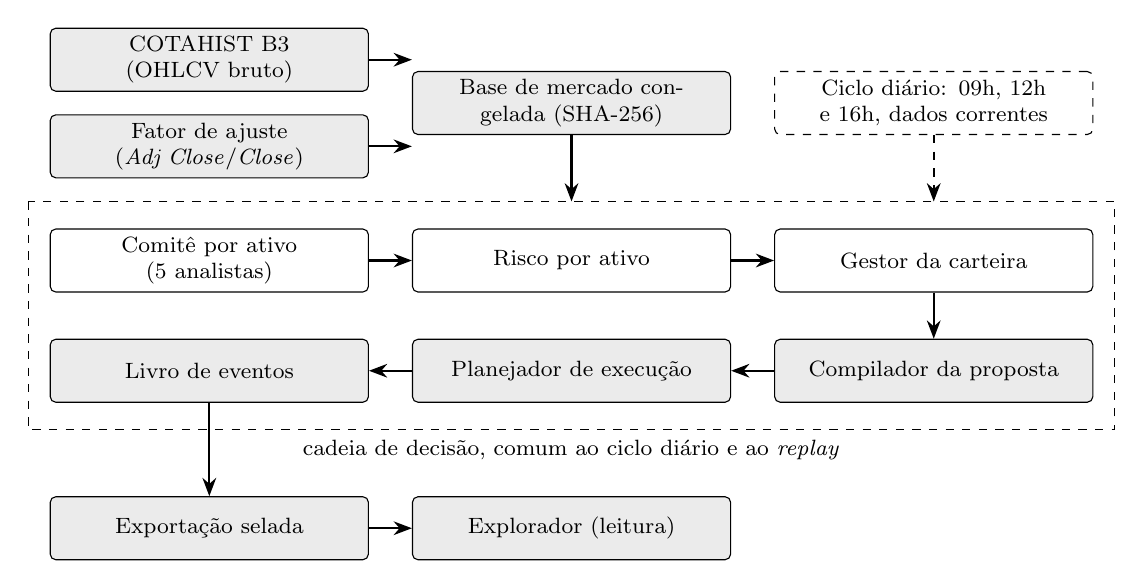
\begin{tikzpicture}[
  box/.style={draw, rounded corners=2pt, minimum height=8mm, text width=3.9cm, align=center, inner sep=2pt, font=\footnotesize},
  det/.style={box, fill=black!8},
  arr/.style={-Stealth, thick},
]
\node[det] (cota) at (-4.6, 0.55) {COTAHIST B3 (OHLCV bruto)};
\node[det] (fator) at (-4.6, -0.55) {Fator de ajuste (\textit{Adj Close}/\textit{Close})};
\node[det] (base) at (0, 0) {Base de mercado congelada (SHA-256)};
\node[box, dashed] (ciclo) at (4.6, 0) {Ciclo diário: 09h, 12h e 16h, dados correntes};
\draw[arr] (cota.east) -- (base.west |- cota.east);
\draw[arr] (fator.east) -- (base.west |- fator.east);
\draw[dashed] (-6.9, -1.25) rectangle (6.9, -4.15);
\node[box] (com) at (-4.6, -2.0) {Comitê por ativo (5 analistas)};
\node[box] (ris) at (0, -2.0) {Risco por ativo};
\node[box] (ges) at (4.6, -2.0) {Gestor da carteira};
\node[det] (comp) at (4.6, -3.4) {Compilador da proposta};
\node[det] (plan) at (0, -3.4) {Planejador de execução};
\node[det] (livro) at (-4.6, -3.4) {Livro de eventos};
\node[font=\footnotesize] at (0, -4.4) {cadeia de decisão, comum ao ciclo diário e ao \textit{replay}};
\node[det] (exp) at (-4.6, -5.4) {Exportação selada};
\node[det] (expl) at (0, -5.4) {Explorador (leitura)};
\draw[arr] (base.south) -- (0, -1.25);
\draw[arr, dashed] (ciclo.south) -- (4.6, -1.25);
\draw[arr] (com) -- (ris);
\draw[arr] (ris) -- (ges);
\draw[arr] (ges) -- (comp);
\draw[arr] (comp) -- (plan);
\draw[arr] (plan) -- (livro);
\draw[arr] (livro) -- (exp);
\draw[arr] (exp) -- (expl);
\end{tikzpicture}
\caption{Componentes do Hedge-fund-lab. Caixas sombreadas são etapas determinísticas; caixas brancas envolvem chamadas ao modelo de linguagem. O retângulo tracejado delimita a cadeia de decisão, alimentada pela base congelada (\textit{replay}) ou pelo ciclo diário (tracejado).}
\label{fig:componentes}
{\footnotesize Fonte: elaborado pelos autores.}
\end{figure}

O sistema é escrito em Python, sem framework web; as tecnologias estão listadas no Apêndice~\ref{ap:mapa}.

\section{Dados}
\label{sec:arq-dados}

A fonte científica de preço é o arquivo oficial de cotações históricas da B3 (COTAHIST, mercado à vista), combinado a um fator de ajuste por sessão, derivado da razão entre o preço de fechamento ajustado e o reportado (\textit{Adj Close}/\textit{Close}) obtida do \texttt{yfinance}. A composição resulta em uma representação de retorno total ajustada por proventos. O calendário de negociação é modelado pela classe \texttt{B3Calendar}, que aplica as regras históricas de feriados da B3 e reproduz as sessões oficiais.

% Fonte: dashboard/market_base_api.py; scripts/continuous_replay_data.py; scripts/replay_multiasset.py; DP-27.
A carteira multiativos utiliza uma base de mercado local dos cinco ativos (\mbox{DP-27}), que separa duas representações por sessão: o OHLCV bruto (RAW) do COTAHIST, empregado na marcação a mercado e na execução simulada, e o fator de ajuste, empregado apenas no cálculo dos indicadores e dos sinais. Essa separação impede que um preço ajustado retroativamente altere a contabilidade. Para o Replay Contínuo, a base é congelada em um \textit{bundle} da campanha, com o \textit{hash} SHA-256 dos arquivos e o instante de aquisição. Os fatores de ajuste foram adquiridos depois do período e, portanto, não constituem uma representação \textit{point-in-time}; a Seção~\ref{sec:arq-multiativos} mostra que isso não altera os sinais entregues aos agentes.

\section{Livro Contábil de Eventos}
\label{sec:arq-livro}

% Fonte: dashboard/manual_portfolio_api.py.
As carteiras simuladas utilizam um livro contábil de eventos, distinto do banco das séries. Cada criação de carteira, operação, provento recebido ou recibo de decisão é gravado como um evento imutável, que armazena o \textit{hash} do evento anterior da mesma carteira e forma uma cadeia verificada a cada leitura. Cada comando possui identificador único, o que torna idempotente a repetição de uma gravação. Posições, caixa e base de custo não são armazenados como saldos: são recalculados a cada leitura pela reprodução ordenada dos eventos (\textit{event sourcing}). Valores monetários são tratados com \texttt{Decimal} e arredondados a centavos. Os detalhes de persistência estão no Apêndice~\ref{ap:mapa}.

\section{Carteira Multiagente Multiativos}
\label{sec:arq-multiativos}

% Fonte: scripts/multiasset_radar.py (technical_input, committee, RISK_PROMPT);
% dashboard/wallet_manager_api.py (PROMPT, Proposal, compile_proposal);
% dashboard/auction_orders.py (plan); scripts/continuous_replay.py (execute).
A carteira opera um universo fixo de cinco ações da B3 (BBAS3, ITUB4, PETR4, VALE3 e WEGE3) com caixa compartilhado. A decisão de cada pregão é organizada em quatro etapas: um comitê de analistas por ativo, um analista de risco por ativo, um gestor global da carteira e um compilador determinístico da proposta. Na configuração do Replay Contínuo, todos os papéis baseados em modelo de linguagem empregam \texttt{gemini-3.8-flash}, com temperatura 1,0, nível de raciocínio baixo e até 8.192 \textit{tokens} de saída. A Figura~\ref{fig:fluxo-multiativos} resume o fluxo de um pregão.

\subsection{Comitê de analistas por ativo}

O comitê por ativo é implementado no Radar multiativos. A preparação da entrada valida o OHLCV, exige histórico mínimo de 200 sessões, verifica a igualdade entre as datas das barras e a grade do \texttt{B3Calendar}, recusa sessões sem negociação e calcula as oito \textit{features} adimensionais da Tabela~\ref{tab:features}, além da volatilidade anualizada dos últimos 21 retornos diários.

\begin{table}[H]
\centering
\caption{Features entregues aos analistas. $P_t$ é o fechamento ajustado da sessão de referência; $\mathrm{SMA}_n$ é a média móvel simples de $n$ sessões; $\mathrm{BB}^{\pm}=\mathrm{SMA}_{20}\pm 2\,\sigma_{20}$, com $\sigma_{20}$ o desvio-padrão amostral das 20 últimas sessões.}
\label{tab:features}
\small
\setlength{\tabcolsep}{4pt}
\begin{tabular}{>{\raggedright\arraybackslash}p{2.9cm} >{\raggedright\arraybackslash}p{4.4cm} >{\raggedright\arraybackslash}p{2.6cm} >{\raggedright\arraybackslash}p{4.6cm}}
\toprule
\textbf{Feature} & \textbf{Fórmula} & \textbf{Janela} & \textbf{Sinal} \\
\midrule
\texttt{rsi} & $100\,G_t/(G_t+L_t)$, com $G_t$ e $L_t$ os ganhos e perdas médios de Wilder & 14 sessões & Escala de 0 a 100; valores altos indicam predomínio de ganhos recentes \\
\texttt{sma50\_gap} & $P_t/\mathrm{SMA}_{50,t}-1$ & 50 sessões & Positivo com o preço acima da média \\
\texttt{sma200\_gap} & $P_t/\mathrm{SMA}_{200,t}-1$ & 200 sessões & Positivo com o preço acima da média \\
\texttt{bb\_upper\_gap} & $P_t/\mathrm{BB}^{+}_t-1$ & 20 sessões & Negativo com o preço abaixo da banda superior \\
\texttt{bb\_lower\_gap} & $P_t/\mathrm{BB}^{-}_t-1$ & 20 sessões & Positivo com o preço acima da banda inferior \\
\texttt{bb\_width} & $(\mathrm{BB}^{+}_t-\mathrm{BB}^{-}_t)/\mathrm{SMA}_{20,t}$ & 20 sessões & Sempre não negativo \\
\texttt{macd\_ratio} & $\mathrm{MACD}_t/P_t$, com $\mathrm{MACD}=\mathrm{EMA}_{12}-\mathrm{EMA}_{26}$ & Recursiva (12 e 26) & Positivo com o MACD acima de zero \\
\texttt{macd\_signal\_ratio} & $S_t/P_t$, com $S=\mathrm{EMA}_9(\mathrm{MACD})$ & Recursiva (9) & Comparada a \texttt{macd\_ratio}: o MACD está acima da linha de sinal se \texttt{macd\_ratio} é maior \\
\bottomrule
\end{tabular}
\end{table}

Todas as oito \textit{features} são razões invariantes à escala: multiplicar todo o histórico de preços por uma constante positiva não altera nenhuma delas. Por isso, um fator de ajuste posterior, que multiplica igualmente toda a janela de cálculo, não altera os sinais; apenas proventos com data-com dentro da janela, já conhecidos em $t-1$, modificam a série. O contrato de \textit{features} do código garante essa invariância e quantiza os valores em seis casas decimais antes de enviá-los ao provedor.

O comitê reutiliza o nó de comitê técnico de \texttt{src/agents} com cinco analistas, \textit{prompt} técnico versão 5, sementes 10001 a 10005, limiar de consenso 0,6 e exigência de voto válido de todos os analistas. Cada voto é uma resposta estruturada com sinal (COMPRA, VENDA ou MANTER), confiança autodeclarada e códigos de evidência restritos ao vocabulário permitido para as \textit{features} recebidas. Com limiar 0,6, o consenso exige ao menos três votos no mesmo sinal; na ausência de consenso, o sinal encaminhado é MANTER com confiança nula. Os analistas e o analista de risco recebem apenas \textit{features} adimensionais (e, o segundo, métricas de risco do ativo): ticker, data e preço não entram em seus \textit{prompts}, nem as posições da carteira, o que fecha, nessas etapas, o canal de memorização do período. Apenas o gestor recebe tickers, datas e preços.

\subsection{Analista de risco por ativo}

O risco é avaliado por ativo, sem conhecimento da carteira. Quando a volatilidade anualizada de 21 dias supera 50\%, uma regra determinística emite o veredito \texttt{VETADO} sem chamada ao modelo. Caso contrário, uma chamada consultiva recebe o sinal consolidado, as \textit{features} e a volatilidade, e devolve \texttt{APROVADO} ou \texttt{VETADO}. O \textit{prompt} proíbe inventar concentração, caixa, posições ou \textit{drawdown} da carteira; o risco agregado é registrado como não avaliado. Na versão original, a recomendação encaminhada ao gestor é o sinal técnico quando o risco aprova e MANTER quando veta.

\subsection{Gestor global da carteira}

O gestor recebe um contexto canônico com a carteira (posições e caixa), a sessão de referência, o dia-alvo, os preços de fechamento RAW da sessão de referência, os pareceres dos cinco ativos e a taxa de custo declarada, e devolve uma única resposta coordenada para o capital compartilhado. A resposta contém um resumo, uma lista de ações e uma lista de riscos; cada ação traz \textit{ticker}, lado (\texttt{BUY}, \texttt{SELL} ou \texttt{HOLD}), quantidade inteira e justificativa. O \textit{prompt} exige exatamente uma ação por ativo, trata os pareceres como dados e não como instruções, proíbe crédito, venda a descoberto e frações, e permite manter caixa.

\subsection{Compilador determinístico da proposta}

A resposta do gestor não é aplicada diretamente. O compilador valida-a contra o esquema e aplica, em ordem (vendas, manutenções, compras), as regras: universo completo e sem \textit{tickers} repetidos; \texttt{HOLD} com quantidade zero; compra apenas com recomendação COMPRA e risco \texttt{APROVADO}; venda apenas com recomendação VENDA e risco \texttt{APROVADO}; venda limitada à posição; caixa nunca negativo após custos. O resultado é uma tabela antes/depois por ativo (quantidade, valor e peso), a lista de operações e o patrimônio projetado. Na versão original, qualquer violação interrompe a compilação, e o pregão é registrado sem operações (Seção~\ref{sec:arq-replay}); as versões posteriores alteram esse comportamento (Seção~\ref{sec:arq-evolucao}).

\subsection{Planejamento da execução e livro}

A cesta compilada é convertida em operações por um planejador. As vendas são processadas primeiro; se o caixa resultante não cobrir as compras, todas as compras são reduzidas pelo mesmo fator em ações inteiras e, persistindo a insuficiência, a maior compra perde uma ação por vez até caber. Um ativo sem preço oficial não é executado, sem substituição por outro preço. A origem de cada operação registra quatro preços (decisão, prévia, aprovação e leilão), o que permite medir o custo de implementação. As operações são gravadas no livro em uma única transação, mediante prévia e confirmação por \textit{token}.

\begin{figure}[htbp]
\centering
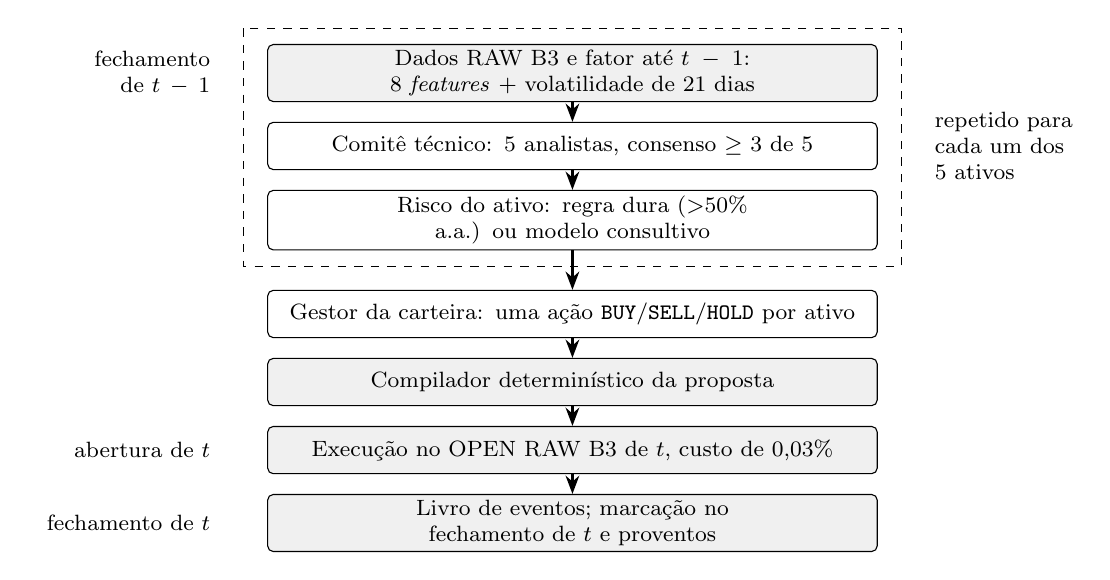
\begin{tikzpicture}[
  node distance=2.5mm,
  box/.style={draw, rounded corners=2pt, minimum height=6mm, text width=7.6cm, align=center, inner sep=2pt, font=\footnotesize},
  det/.style={box, fill=black!6},
  note/.style={font=\footnotesize, align=right, text width=2.2cm},
  arr/.style={-Stealth, thick},
]
\node[det] (feat) {Dados RAW B3 e fator até $t-1$: 8 \textit{features} + volatilidade de 21 dias};
\node[box, below=of feat] (comite) {Comitê técnico: 5 analistas, consenso $\geq$ 3 de 5};
\node[box, below=of comite] (risco) {Risco do ativo: regra dura ($>$50\% a.a.) ou modelo consultivo};
\node[box, below=5mm of risco] (gestor) {Gestor da carteira: uma ação \texttt{BUY}/\texttt{SELL}/\texttt{HOLD} por ativo};
\node[det, below=of gestor] (comp) {Compilador determinístico da proposta};
\node[det, below=of comp] (exec) {Execução no OPEN RAW B3 de $t$, custo de 0,03\%};
\node[det, below=of exec] (marca) {Livro de eventos; marcação no fechamento de $t$ e proventos};
\draw[arr] (feat) -- (comite);
\draw[arr] (comite) -- (risco);
\draw[arr] (risco) -- (gestor);
\draw[arr] (gestor) -- (comp);
\draw[arr] (comp) -- (exec);
\draw[arr] (exec) -- (marca);
\draw[dashed] ([xshift=-3mm, yshift=2mm]feat.north west) rectangle ([xshift=3mm, yshift=-2mm]risco.south east);
\node[font=\footnotesize, align=left, anchor=west] at ([xshift=6mm]comite.east) {repetido para\\cada um dos\\5 ativos};
\node[note, anchor=east] at ([xshift=-6mm]feat.west) {fechamento\\de $t-1$};
\node[note, anchor=east] at ([xshift=-6mm]exec.west) {abertura de $t$};
\node[note, anchor=east] at ([xshift=-6mm]marca.west) {fechamento de $t$};
\end{tikzpicture}
\caption{Fluxo de um pregão $t$ na carteira multiagente multiativos. Caixas sombreadas são etapas determinísticas; caixas brancas envolvem chamadas ao modelo de linguagem (a etapa de risco apenas quando a regra dura não se aplica). O retângulo tracejado indica as etapas executadas por ativo.}
\label{fig:fluxo-multiativos}
{\footnotesize Fonte: elaborado pelos autores.}
\end{figure}

\section{Relógio Causal do Pregão}
\label{sec:arq-relogio}

% Fonte: scripts/replay_multiasset.py (prepare, LIMITATIONS); scripts/continuous_replay*.py
% (execute, preflight); dashboard/auction_orders.py (plan); dashboard/dividends_api.py (JCP_NET).
O tratamento temporal de cada pregão-alvo $t$ separa a informação disponível para a decisão da informação usada para executar e avaliar:

\begin{enumerate}
  \item \textbf{Decisão com dados até $t-1$.} A entrada de cada ativo é construída a partir das barras compreendidas entre 450 dias corridos antes da sessão de referência e a própria sessão de referência, que é o pregão imediatamente anterior a $t$.  \item \textbf{Aprovação hipotética às 09:00 de $t$.} No \textit{replay}, a cesta compilada é considerada aprovada antes da abertura, sem a prévia com cotação atrasada, o alerta de tese desatualizada e as tentativas das 12:00 e 16:00 do ciclo diário (Seção~\ref{sec:arq-operacao-diaria}).
  \item \textbf{Execução no OPEN RAW B3 de $t$.} O preço de execução é a abertura oficial bruta do COTAHIST (campo PREABE), usada como aproximação diária do leilão de abertura, sem \textit{spread}, impacto, livro de ofertas ou liquidação em D+2. Cada operação posterior à entrada paga custo de 0,03\% sobre o valor bruto; não há custo fixo nem lote mínimo de bolsa.
  \item \textbf{Marcação no fechamento de $t$.} As carteiras são marcadas ao fechamento RAW B3 de $t$. Os proventos seguem a \mbox{DP-30}: o direito é determinado pela posição na data-com, o JCP é creditado líquido de 15\% de imposto e o valor só entra no caixa na data de pagamento; entre as duas datas, aparece como recebível, que compõe o patrimônio mas não o caixa disponível para compras. O caixa não é remunerado.
\end{enumerate}

Os sinais das carteiras de referência utilizam o fechamento B3 multiplicado pelo fator de ajuste; operações e patrimônio de todas as carteiras utilizam preços RAW.

A proteção contra antecipação de informação (\textit{look-ahead}) atua em três pontos. Primeiro, a entrada é truncada na sessão de referência, e um verificador adultera barras futuras para conferir que as entradas permanecem idênticas. Segundo, antes de qualquer chamada, uma verificação preliminar executada sob bloqueio de rede percorre todas as entradas da campanha e interrompe a execução se alguma sessão de entrada for igual ou posterior ao dia-alvo. Terceiro, imediatamente antes de cada requisição HTTP, a entrada é relida e comparada com a versão registrada; qualquer diferença interrompe a campanha, e o mesmo vale para o contexto do gestor. Os códigos de erro correspondentes estão no Apêndice~\ref{ap:mapa}. Esses controles garantem a causalidade dos dados entregues aos agentes, mas não eliminam a possibilidade de o modelo conhecer o período por seu treinamento; essa limitação é tratada no Capítulo~\ref{cha:metodologia}.

\section{Carteiras de Referência}
\label{sec:arq-referencias}

Os indicadores técnicos (médias móveis simples, Bandas de Bollinger, RSI de Wilder e MACD) e as estratégias clássicas são módulos próprios do repositório, reutilizados pelo caminho multiativos por meio de adaptadores. O Replay Contínuo não utiliza o motor de \textit{backtesting} clássico (Apêndice~\ref{ap:ativo-unico}): as seis carteiras evoluem no livro de eventos, com execução, custos e proventos aplicados pelos módulos da aplicação. Do motor, reutilizam-se o calendário B3 e as classes de alocação por pesos.

% Fonte: scripts/continuous_replay.py (initialize, references); dashboard/rule_portfolios.py.
As seis carteiras partem de uma mesma cesta inicial (\mbox{DP-20}), criada no livro em uma única transação: 20\% do capital por ativo em ações inteiras, ao fechamento da sessão anterior ao primeiro pregão, com custo zero, registrada como posição inicial, sem simular execução a mercado. As cinco referências são calculadas integralmente antes do laço de inferência, sem chamadas ao modelo e, nas versões v2 e v3, sob bloqueio de rede:

\begin{itemize}
  \item \textbf{\textit{Buy \& Hold}:} mantém a cesta inicial, sem rebalanceamento.
  \item \textbf{SMA 50/200 e Bollinger 20/2:} aplicam o cruzamento de médias de 50 e 200 sessões e as Bandas de Bollinger de 20 sessões e 2 desvios a parcelas independentes de 20\% do capital por ativo, decidindo no fechamento de $t-1$ e executando na abertura de $t$.
  \item \textbf{Pesos iguais e mínima variância:} recalculados a cada 63 pregões; a mínima variância usa janela de 252 retornos e somente posições compradas. Os pesos são convertidos em quantidades inteiras à abertura e executados pelo mesmo planejador da carteira Multiagentes. Os pesos, a janela e o resultado do otimizador ficam registrados no recibo de decisão.
\end{itemize}

Em todas as referências, os proventos permanecem em caixa, sem reinvestimento. A igualdade das referências entre as três campanhas é conferida por auditoria posterior.

\section{Mecanismo do Replay Contínuo}
\label{sec:arq-replay}

% Fonte: scripts/continuous_replay.py, continuous_replay_v2.py, continuous_replay_v3.py,
% continuous_replay_runtime.py, continuous_replay_dividends.py, export_continuous_replay*.py,
% build_replay_explorer.py, publish_replay.py, dashboard/server.py (_serve_replay).
O Replay Contínuo Abril--Novembro de 2026 reconstitui, em uma única trajetória sem reinício, 153 pregões da B3 (06/04/2026 a 12/11/2026) para seis carteiras independentes de R\$~100.000,00: a carteira Multiagentes e as cinco referências. É uma reconstrução retrospectiva, produzida após o fim do período, autorizada como extensão do projeto (\mbox{DP-37}), com a v1 pré-especificada e a v2 e a v3 exploratórias. O desenho experimental é apresentado no Capítulo~\ref{cha:metodologia} e os resultados, no Capítulo~\ref{cha:resultados}; esta seção descreve o mecanismo que os produz.

\subsection{Execução, identidade e isolamento}

Cada geração possui um executor, uma raiz de armazenamento, um livro, um orçamento e um pacote exportado próprios. As versões v2 e v3 consomem as mesmas entradas congeladas da v1, conferindo o \textit{hash} do \textit{bundle} de mercado antes do uso, e reutilizam contabilidade, livro, planejador, transporte e orçamento sem editar as fontes das versões anteriores. No início de cada execução, o executor grava um manifesto da campanha com a identidade, o modo (inferência real ou teste \textit{offline}), as sessões, as estratégias, o teto de orçamento e os \textit{hashes} SHA-256 das fontes utilizadas. Se já existir um manifesto diferente, a execução é recusada, o que impede retomar uma campanha com código ou dados distintos dos que a iniciaram. Um \textit{lock} exclusivo impede dois executores simultâneos sobre a mesma raiz.

\subsection{Laço diário e semântica \textit{fail-closed}}

Para cada pregão, o executor grava artefatos intermediários selados, nesta ordem: o estado das carteiras antes do pregão; o resultado do comitê de cada ativo, com a entrada e o diário de chamadas; o contexto e a proposta compilada do gestor; o plano de execução; e o fechamento do dia, com a marcação das seis carteiras. A existência de cada artefato faz com que a etapa correspondente seja reaproveitada em vez de reexecutada, de modo que uma interrupção é retomada no mesmo ponto, sem nova chamada ao modelo para etapas já concluídas.

Quando o comitê de algum ativo não se completa ou a proposta do gestor não pode ser compilada, o pregão é registrado como \texttt{NO\_ANALYSIS}: nenhuma operação é gravada, as posições vigentes são preservadas, as seis carteiras são marcadas normalmente e a campanha prossegue. Votos parciais recebidos permanecem registrados, e nenhuma decisão é fabricada para preencher a lacuna. Erros de integridade do diário ou do orçamento, ao contrário, interrompem a campanha.

\subsection{Orçamento e diário de chamadas}

Cada campanha possui um teto agregado de US\$~34,78, registrado no manifesto, que inclui tentativas repetidas, chamadas em andamento e respostas sem uso conhecido. Antes de cada tentativa HTTP, grava-se em SQLite uma reserva com o custo máximo da chamada, calculado pelos limites de \textit{bytes} de entrada e \textit{tokens} de saída às tarifas mais altas anunciadas pelo provedor; se a reserva ultrapassar o teto, a campanha é interrompida. Ao receber a resposta, o custo é estimado pelos \textit{tokens} informados pelo provedor. Os valores de reserva e as tarifas estão no Apêndice~\ref{ap:mapa}. A estimativa não substitui a fatura do provedor.

Cada chamada lógica admite no máximo duas tentativas físicas, apenas para falhas de transporte. Uma resposta já recebida e persistida é sempre reutilizada, inclusive após interrupção, e nunca solicitada novamente; esgotadas as duas tentativas, não há substituição automática. Cada comitê e cada gestor possuem um diário de chamadas, com requisições, envelopes brutos e respostas validadas, exportado ao final. Uma auditoria do orçamento reconstrói todas as tentativas, confere o \textit{hash} de cada envelope, recalcula o custo e verifica que nenhuma chamada lógica teve mais de duas tentativas ou mais de uma resposta consumida. A reprodução dos resultados parte das respostas arquivadas no diário; uma nova inferência, mesmo com as mesmas sementes e temperatura 1,0, não garante respostas idênticas.

\subsection{Exportação e consulta}

Ao final, os exportadores leem os recibos gravados, sem inferência nem alteração do livro, e produzem um pacote selado por \textit{hash} com sessões, carteiras, pareceres, operações, chamadas arquivadas, tabelas CSV e uma página HTML autônoma. O pacote é instalado no servidor apenas se coincidir com o \textit{hash} fixado no código para a versão, e é consultado por rotas somente de leitura que não executam agentes nem operações (Apêndice~\ref{ap:empacotamento}).
\section{Evolução da Arquitetura entre Versões}
\label{sec:arq-evolucao}

% Fonte: scripts/continuous_replay_v2.py (constantes, LENTE_*, committee_v2, PROMPT_V2,
% compile_proposal_v2); scripts/continuous_replay_v3.py (constantes, _LENS_SUFFIX,
% committee_v3, PROMPT_V3, compute_position_memory, compile_proposal_v3).
As três gerações mantêm a mesma topologia de agentes por pregão --- cinco analistas por ativo, até um analista de risco por ativo e um gestor, no máximo 31 chamadas ---, o mesmo modelo e configuração de geração, as mesmas \textit{features}, a mesma regra dura de volatilidade, o mesmo \textit{prompt} de risco e o mesmo esquema de resposta do gestor. Também são comuns a execução, os custos, os proventos, o orçamento e as cinco referências. Variam a composição do comitê, a regra de agregação e de veto, o contexto e as regras do gestor e o comportamento do compilador, conforme a Tabela~\ref{tab:evolucao-versoes}. Os resultados de cada versão são apresentados no Capítulo~\ref{cha:resultados}.

\begin{table}[htbp]
\centering
\caption{Diferenças arquiteturais entre as três gerações da carteira Multiagentes no Replay Contínuo.}
\label{tab:evolucao-versoes}
\small
\setlength{\tabcolsep}{4pt}
\begin{tabular}{>{\raggedright\arraybackslash}p{3.0cm} >{\raggedright\arraybackslash}p{3.8cm} >{\raggedright\arraybackslash}p{3.8cm} >{\raggedright\arraybackslash}p{4.0cm}}
\toprule
\textbf{Dimensão} & \textbf{v1} & \textbf{v2} & \textbf{v3} \\
\midrule
\textit{Prompt} dos analistas & Um único \textit{prompt} (v5) para os cinco & \textit{Prompt} base + 3 lentes (2 + 2 + 1) & \textit{Prompt} base + 5 lentes distintas \\
Travas sobre o consenso & Não & Não & Reversão de consensos 3--2 em extremos \\
Efeito do veto de risco & \texttt{VETADO} $\rightarrow$ MANTER & \texttt{VETADO} bloqueia só compras (R7) & Igual à v2 \\
Contexto do gestor & Carteira, preços e pareceres & Igual à v1 & Acrescenta memória de posição \\
\textit{Prompt} do gestor & Original & \texttt{PROMPT\_V2} (4 regras) & \texttt{PROMPT\_V3} (7 regras) \\
Compilador & Estrito: violação invalida o pregão & Ajusta e registra (\texttt{strict=False}) & Ajusta e registra (\texttt{strict=False}) \\
Limites de compra & Caixa disponível & Teto de 30\% e mínimo de R\$~2.000 & Teto de 30\% (22\% em recomposição) e mínimo de R\$~2.000 \\
Vendas parciais fora de VENDA & Não & \textit{Trim-to-Fund} & \textit{Trim-to-Fund} e \textit{Trim-on-Strength} \\
Limites de venda em VENDA & Posição & Posição & 45\% da posição por pregão e piso de 8\% \\
\bottomrule
\end{tabular}
\end{table}

\subsection{Versão v2}

A v2 acrescenta quatro intervenções, impostas tanto no \textit{prompt} do gestor quanto no compilador: o \textit{Trim-to-Fund}, venda parcial de ativo em MANTER ou COMPRA quando o peso supera 25\% do patrimônio; o teto de concentração de 30\% por ativo e a ordem mínima de compra de R\$~2.000,00; o veto assimétrico (R7), em que \texttt{VETADO} bloqueia apenas compras e o consenso de VENDA permanece sob veto; e três lentes analíticas sobre o \textit{prompt} técnico v5 (tendência estrutural, reversão por Bollinger e RSI e regime de volatilidade). O compilador deixa ainda de invalidar o pregão diante de uma violação de regra: em modo não estrito, reduz a quantidade ou converte a ação em \texttt{HOLD} e registra cada ajuste e seu motivo; violações estruturais continuam invalidando o pregão.

\subsection{Versão v3}

A v3 mantém as regras da v2 e acrescenta quatro grupos de mecanismos, parametrizados por constantes determinísticas: cinco lentes especialistas, uma por analista, com duas travas que revertem para MANTER os consensos de exatamente três votos em extremos de RSI e de bandas; memória de posição no contexto do gestor, piso de 8\% de peso, venda escalonada limitada a 45\% da posição por pregão e regra \textit{anti-whipsaw} contra recompra mais cara em oito pregões; realização parcial em força (\textit{Trim-on-Strength}) de ativos esticados e em lucro; e recomposição (\textit{Dip-Rebalance}) quando o caixa supera 25\% do patrimônio. As regras detalhadas e as constantes (Tabela~\ref{tab:constantes-v3}) estão no Apêndice~\ref{ap:mapa}.

As regras de ambas as versões foram formuladas após a observação das campanhas anteriores sobre o mesmo período. Por isso, a v2 e a v3 são iterações exploratórias, ajustadas dentro da amostra, e recebem apenas descrição, não validação independente das regras; essa restrição é discutida nos Capítulos~\ref{cha:metodologia} e~\ref{cha:resultados}. A qualificação de cada versão antes da execução paga foi feita com respostas simuladas do modelo e rede bloqueada; essas verificações atestam o funcionamento do mecanismo e não constituem desempenho dos agentes.

\section{Operação Diária e Interface}
\label{sec:arq-operacao-diaria}

% Fonte: dashboard/daily_cycle.py (docstring, SLOTS, CAP_USD, windows, manager, close_day);
% dashboard/auction_orders.py (first_auction, execution_slot); Dockerfile; railway.json; DP-33/34/35.
Fora do \textit{replay}, a mesma carteira multiativos é operada diariamente sobre dados correntes, em regime de simulação sem capital real e sem envio de ordens a corretoras. O ciclo diário opera a arquitetura da v1; as regras da v2 e da v3 existem apenas nos executores do \textit{replay}. O ciclo autônomo (\mbox{DP-34}) executa dentro do processo do servidor quando habilitado por variável de ambiente. Em cada pregão da B3 há tentativas às 09:00, 12:00 e 16:00 (horário de São Paulo); uma tentativa posterior só ocorre se a anterior não tiver encerrado o dia.

Cada tentativa percorre, chamando as mesmas funções usadas pela interface, as etapas: atualização da base de mercado; abertura de uma análise com dia-alvo no pregão corrente e dados até o último pregão encerrado e publicado; comitês por ativo; contexto e chamada do gestor; prévia com cotação atrasada; e aprovação automática, exceto quando o \textit{backend} emite alerta de tese desatualizada, caso em que a cesta aguarda revisão humana. As reservas de custo do dia são limitadas a US\$~4,00. Cada tentativa gera um registro selado e imutável, e o dia é encerrado em um de três estados: concluído, aguardando revisão humana ou sem análise; um dia encerrado não é executado novamente.
A execução segue as regras de leilão das \mbox{DP-33} e \mbox{DP-35}: uma aprovação anterior ao corte de abertura executa no OPEN oficial B3 do dia; uma aprovação durante o pregão executa ao preço de abertura da primeira barra de um minuto do Yahoo Finance posterior à aprovação. A cotação atrasada é usada somente na prévia, nunca na marcação nem no \textit{prompt} do gestor. O \textit{replay} reutiliza os módulos desse ciclo, mas simplifica o relógio para uma aprovação hipotética às 09:00 com execução no OPEN (Seção~\ref{sec:arq-relogio}).

\begin{figure}[htbp]
\centering
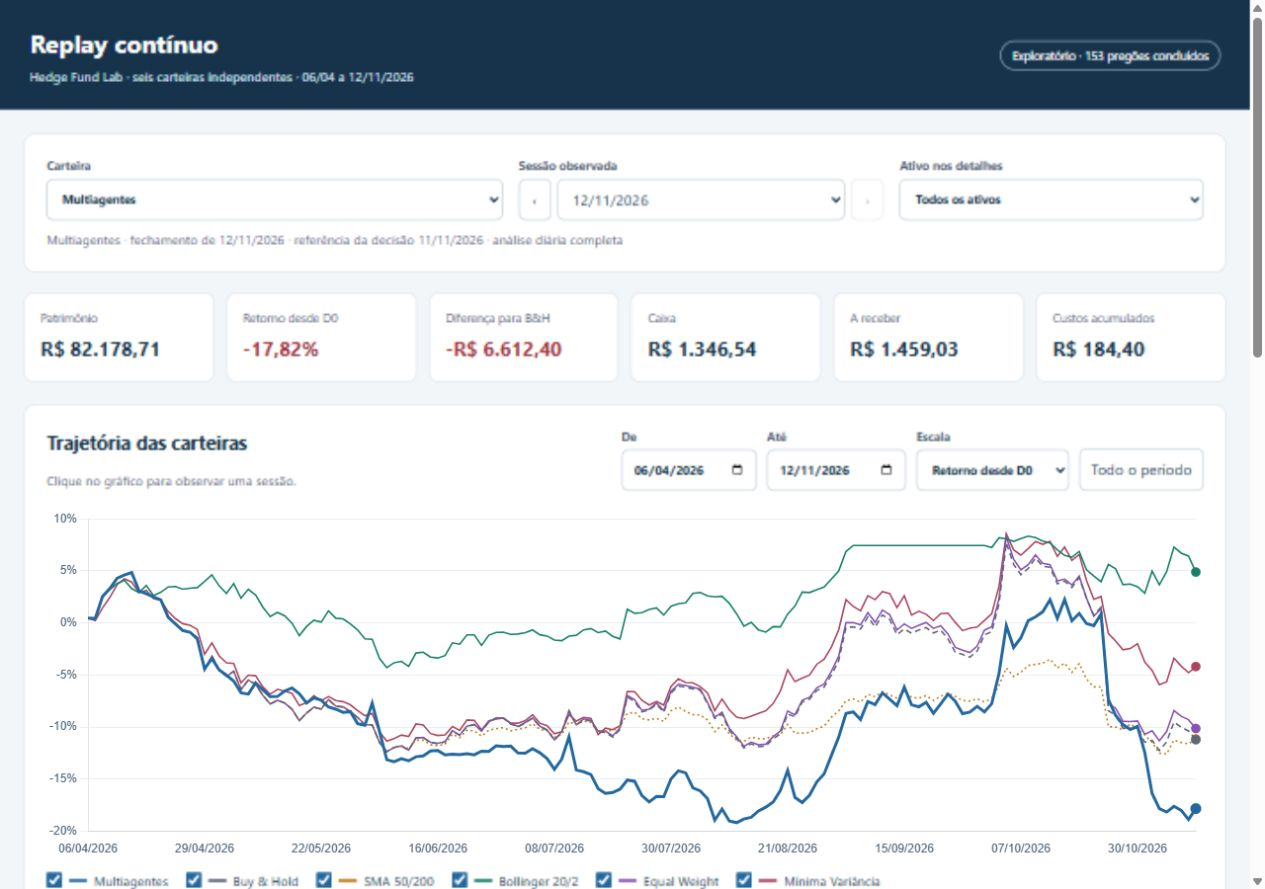
\includegraphics[width=0.85\textwidth]{images/explorador-replay.jpg}
\caption{Explorador do Replay Contínuo (v1), na sessão de 12/11/2026: seletores de carteira, sessão e ativo; patrimônio, retorno desde D0, diferença para o \textit{Buy \& Hold}, caixa, valores a receber e custos acumulados da carteira Multiagentes; e curvas de retorno das seis carteiras de 06/04 a 12/11/2026.}
\label{fig:explorador}
{\footnotesize Fonte: captura de tela do explorador, elaborada pelos autores.}
\end{figure}

A aplicação é empacotada em contêiner e executada em um servidor pessoal em nuvem, com volume persistente e acesso apenas por rede privada, sem exposição pública. A interface é implementada com HTML, CSS e JavaScript, servida por um servidor HTTP da biblioteca padrão que valida \texttt{Host} e \texttt{Origin}, \textit{token} CSRF e JSON estrito nas requisições que alteram estado. A navegação tem a carteira como tela inicial e reúne as áreas Carteira, Operações, Agentes, Comparação, Replay abril--novembro (com acesso às versões v1, v2 e v3), Laboratório, Legacy e Auditoria. A Figura~\ref{fig:explorador} mostra o explorador do \textit{replay}, de onde se acessam posições, votos, pareceres, operações e chamadas arquivadas de cada pregão. A interface apenas apresenta valores calculados no \textit{backend} e não é, por si, objeto da avaliação comparativa descrita no Capítulo~\ref{cha:metodologia}.


\chapter{Metodologia Experimental}
\label{cha:metodologia}

% Fontes: tcc2/evidence/04-replay-abril-novembro/relatorios/evolucao_replay_v1_v2_v3_tcc.md
% (seções 1 e 6); replay_continuo_2026-04_2026-11.md; inventario_replay_continuo_2026-11-13.md;
% REPLAY_MULTIATIVOS.md; tcc2/evidence/03-metodo-h2/; DIRECAO_DO_PROJETO.md (DP-20, DP-31,
% DP-36, DP-37); src/experiments/h2_evaluation.py; src/backtesting/metrics.py;
% tcc2/agent-reports/METRICAS_REPLAY.md.
Este capítulo descreve o desenho experimental pelo qual as hipóteses do trabalho são respondidas. O estudo empírico é o Replay Contínuo Abril--Novembro de 2026, no qual a carteira multiagente multiativos e cinco carteiras de referência determinísticas percorrem a mesma trajetória de mercado, em três versões sucessivas da carteira Multiagentes (v1, v2 e v3). A arquitetura que produz as carteiras, o relógio causal de cada pregão e as diferenças entre as versões estão descritos no Capítulo~\ref{cha:arquitetura} (Seções~\ref{sec:arq-multiativos}, \ref{sec:arq-relogio}, \ref{sec:arq-replay} e~\ref{sec:arq-evolucao}); este capítulo trata do que é comparado, como é medido, como é decidido estatisticamente e de que forma cada escolha limita as conclusões. O protocolo confirmatório planejado originalmente, que não chegou a ser executado, é apresentado de forma condensada na Seção~\ref{sec:met-protocolo}.

\section{Caracterização da Pesquisa}
\label{sec:met-caracterizacao}

A pesquisa é aplicada, de abordagem quantitativa e de caráter comparativo. O método é a simulação retrospectiva (\textit{replay}) de um processo de decisão com inferência real do modelo de linguagem sobre um período fechado: as decisões da carteira Multiagentes resultam de chamadas efetivas ao \texttt{gemini-3.8-flash}, e não de respostas simuladas. As respostas simuladas e a rede bloqueada foram usadas apenas para qualificar o mecanismo antes de cada execução paga (Seção~\ref{sec:arq-evolucao}) e não integram nenhum resultado.

O desenho é pareado: todas as carteiras partem do mesmo estado, são avaliadas nas mesmas sessões, sob os mesmos preços de execução e marcação e sob o mesmo custo de negociação, de modo que as diferenças observadas são atribuíveis às regras de decisão, condicionalmente à trajetória e à execução observadas. Duas perguntas organizam o estudo. A primeira corresponde às hipóteses herdadas do TCC 1 (Seção~\ref{sec:met-hipoteses}). A segunda é arquitetural e descritiva: mantidos o modelo, a quantidade de agentes, os dados e a execução, quanto do comportamento da carteira multiagente depende da especialização dos analistas e das regras determinísticas aplicadas sobre a proposta do gestor. A primeira pergunta é respondida principalmente pela versão v1; a segunda, pela comparação entre as três versões.

O replay foi produzido em novembro de 2026, depois do fim do período simulado, como extensão retrospectiva autorizada pela \mbox{DP-37}, que reabre a \mbox{DP-31} apenas para essa reconstrução e não afirma ausência de contaminação do modelo. Essa natureza retrospectiva é a principal restrição do estudo e condiciona a leitura de todos os resultados (Seção~\ref{sec:met-ameacas}). O estatuto das versões difere: a v1 é pré-especificada e recebe decisão inferencial, condicionada à possível contaminação do modelo; a v2 e a v3 são iterações exploratórias, ajustadas dentro da amostra, e recebem apenas descrição; o acompanhamento prospectivo é a única avaliação livre de contaminação (Seção~\ref{sec:met-prospectivo}).

\section{Do Protocolo Planejado ao Replay}
\label{sec:met-protocolo}

O planejamento original previa avaliar H2 por um protocolo confirmatório com fases em ordem fixa sobre um único ativo (PETR4.SA), cujo Teste Final, isolado e único momento confirmatório, ocuparia a janela proposta de 01/09/2025 a 31/08/2026; o desenho completo está na Subseção~\ref{sec:met-protocolo-detalhes}. Esse protocolo não foi concluído, e o replay o substitui como estudo empírico do trabalho. A Figura~\ref{fig:met-linha-tempo} situa no tempo as janelas planejadas, o corte de conhecimento declarado do modelo e os eventos do replay e do acompanhamento prospectivo.

\begin{figure}[htbp]
\centering
\resizebox{\textwidth}{!}{%
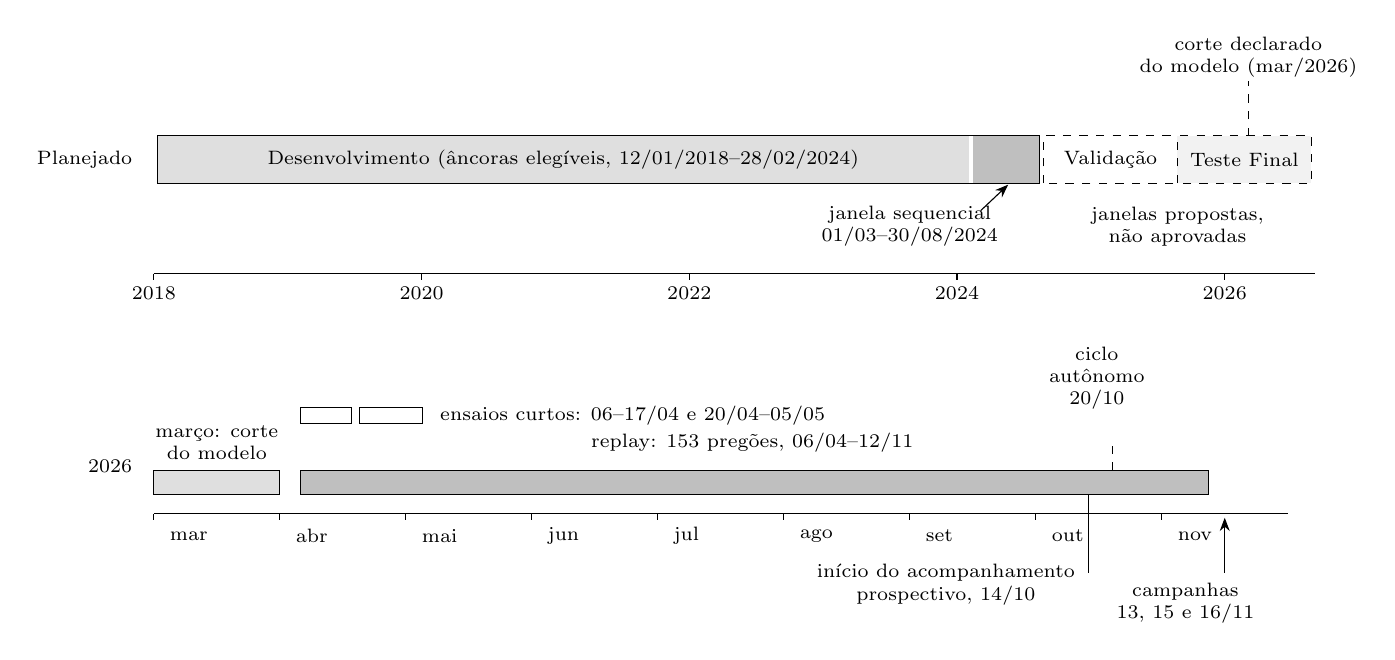
\begin{tikzpicture}[
  lab/.style={font=\scriptsize, align=center},
  seg/.style={draw, minimum height=6mm, inner sep=1pt, font=\scriptsize, align=center},
  mk/.style={font=\scriptsize, align=center},
]
% Escala superior: 1,7 cm por ano, origem em 2018,0
\node[lab, anchor=east] at (-0.15,0) {Planejado};
\fill[gray!25] (0.05,-0.3) rectangle (10.35,0.3);
\fill[gray!50] (10.4,-0.3) rectangle (11.25,0.3);
\draw[dashed, fill=white] (11.3,-0.3) rectangle (13.0,0.3);
\draw[dashed, fill=gray!10] (13.0,-0.3) rectangle (14.7,0.3);
\draw (0.05,-0.3) rectangle (11.25,0.3);
\node[lab] at (5.2,0) {Desenvolvimento (âncoras elegíveis, 12/01/2018--28/02/2024)};
\node[lab] at (12.15,0) {Validação};
\node[lab] at (13.85,0) {Teste Final};
\node[lab] at (9.6,-0.85) {janela sequencial\\01/03--30/08/2024};
\draw[-{Stealth}] (10.5,-0.65) -- (10.85,-0.32);
\foreach \y in {2018,2020,2022,2024,2026}{
  \draw ({1.7*(\y-2018)},-1.45) -- ++(0,-0.08);
  \node[lab] at ({1.7*(\y-2018)},-1.7) {\y};
}
\draw (0,-1.45) -- (14.75,-1.45);
\draw[dashed] (13.9,0.3) -- (13.9,1.0);
\node[mk] at (13.9,1.3) {corte declarado\\do modelo (mar/2026)};
\node[lab] at (13.0,-0.85) {janelas propostas,\\não aprovadas};
% Escala inferior: 2026, 1,6 cm por mês, março = 0
\def\mx#1{(1.6*(#1-3))}
\node[lab, anchor=east] at (-0.15,-3.9) {2026};
\draw (0,-4.5) -- (14.4,-4.5);
\foreach \m/\n in {3/mar,4/abr,5/mai,6/jun,7/jul,8/ago,9/set,10/out,11/nov}{
  \draw ({1.6*(\m-3)},-4.5) -- ++(0,-0.08);
  \node[lab, anchor=west] at ({1.6*(\m-3)+0.08},-4.78) {\n};
}
\fill[gray!25] (0,-4.25) rectangle (1.6,-3.95);
\draw (0,-4.25) rectangle (1.6,-3.95);
\node[lab] at (0.8,-3.6) {março: corte\\do modelo};
\fill[gray!50] ({1.6*(4.167-3)},-4.25) rectangle ({1.6*(11.37-3)},-3.95);
\draw ({1.6*(4.167-3)},-4.25) rectangle ({1.6*(11.37-3)},-3.95);
\node[lab] at (7.6,-3.6) {replay: 153 pregões, 06/04--12/11};
\draw[fill=white] ({1.6*(4.167-3)},-3.35) rectangle ({1.6*(4.567-3)},-3.15);
\draw[fill=white] ({1.6*(4.633-3)},-3.35) rectangle ({1.6*(5.133-3)},-3.15);
\node[lab, anchor=west] at ({1.6*(5.133-3)+0.1},-3.25) {ensaios curtos: 06--17/04 e 20/04--05/05};
\draw ({1.6*(10.42-3)},-4.25) -- ++(0,-1.0);
\node[lab, anchor=east] at ({1.6*(10.42-3)-0.05},-5.4) {início do acompanhamento\\prospectivo, 14/10};
\draw[dashed] ({1.6*(10.61-3)},-3.95) -- ++(0,0.35);
\node[lab, anchor=south] at ({1.6*(10.61-3)-0.2},-3.3) {ciclo\\autônomo\\20/10};
\draw[-{Stealth}] ({1.6*(11.5-3)},-5.25) -- ({1.6*(11.5-3)},-4.55);
\node[lab, anchor=north east] at ({1.6*(11.5-3)+0.5},-5.25) {campanhas\\13, 15 e 16/11};
\end{tikzpicture}%
}
\caption{Linha do tempo do estudo: janelas do protocolo planejado (acima, em anos) e eventos de 2026 (abaixo, em meses). As janelas de Validação e de Teste Final foram apenas propostas.}
\label{fig:met-linha-tempo}
{\footnotesize Fonte: elaborado pelos autores, a partir de \path{docs/DIRECAO_DO_PROJETO.md} (\mbox{DP-31}, \mbox{DP-34} e \mbox{DP-37}) e do texto deste capítulo.}
\end{figure}

A figura mostra que a janela proposta para o Teste Final (09/2025 a 08/2026) começa antes do corte do modelo e se sobrepõe apenas em parte ao replay (04/2026 a 11/2026), que ocorre integralmente depois do corte declarado. As campanhas foram executadas depois do último pregão simulado, e o acompanhamento prospectivo, iniciado em 14/10/2026, é a única avaliação em que cada decisão precede seu desfecho.

As fases de desenvolvimento foram executadas em sucessivas emendas do tratamento, e a Validação foi executada em caráter provisório e descritivo, sem a aprovação formal prevista no protocolo; seus resultados não são usados para decidir as hipóteses (resumo em \path{tcc2/evidence/03-metodo-h2/H2_V6_OA1_VALIDATION_SCIENTIFIC_SUMMARY.md}). O \textit{Freeze} formal e o Teste Final não foram executados, por três razões. Primeiro, as janelas de Validação e de Teste Final e a especificação da camada de avaliação nunca receberam a aprovação formal prevista dos autores e do orientador. Segundo, a \mbox{DP-31} (17/10/2026) estabeleceu que agentes de IA só são avaliados de forma prospectiva, porque a simulação retrospectiva com o modelo é contaminada pelo conhecimento que ele pode ter do desfecho; a janela proposta para o Teste Final termina em agosto de 2026 e, em grande parte, antecede o corte de conhecimento declarado do modelo (março de 2026). Terceiro, três execuções por fase sobre janelas anuais multiplicariam o custo de inferência. Os resultados provisórios desse caminho não são usados para decidir as hipóteses.

Do protocolo, o replay herda a definição do Sharpe, o Bootstrap A, a configuração do comitê técnico e o princípio causal; não herda a separação entre calibração e avaliação, a janela reservada, as três repetições, o universo de ativo único nem a estrutura de custos. O replay é, portanto, o estudo empírico pelo qual as hipóteses são respondidas, com o alcance mais restrito que sua natureza retrospectiva impõe: decisão inferencial apenas para a v1, condicionada à possível contaminação, e descrição para a v2 e a v3.

\subsection{Detalhes do protocolo original}
\label{sec:met-protocolo-detalhes}

O planejamento inicial previa avaliar H2 no caminho de ativo único (Apêndice~\ref{ap:ativo-unico}, Seções~\ref{sec:arq-ativo-unico} e~\ref{sec:arq-experimentos}), sobre PETR4.SA, por um protocolo com fases em ordem fixa e autoridades não cumulativas: \textit{Hardening}, ajuste de configuração sem acesso a métricas financeiras; CAL-A; Desenvolvimento Sequencial; Relatório de Estresse; CAL-B; \textit{Freeze}, congelamento final da configuração; Validação, descritiva; e Teste Final, isolado e único momento confirmatório. O conjunto elegível de âncoras tinha 1.519 sessões, de 12/01/2018 a 28/02/2024, cada uma com ao menos 504 sessões de histórico; o diagnóstico do \textit{Hardening} usava 8 estados sintéticos e 4 sessões reais (\texttt{H\_real}), excluídas dos demais conjuntos. As calibrações usavam um conjunto de 30 âncoras cronológicas (20 para a CAL-A e 10 para a CAL-B, disjuntas) e até oito âncoras de estresse; a janela sequencial (01/03/2024 a 30/08/2024) e as quatro janelas de estresse foram congeladas, enquanto as janelas de Validação (02/09/2024 a 29/08/2025) e de Teste Final (01/09/2025 a 31/08/2026) foram apenas propostas.

A configuração do comitê foi congelada --- \textit{self-consistency} com cinco analistas, limiar de consenso 0,6 e voto obrigatório de todos, \texttt{gemini-3.8-flash} com temperatura 1,0 e até 8.192 \textit{tokens} de saída, peso-alvo determinístico --- e sua integridade era verificada por \textit{hash} fixo da especificação do participante (\texttt{PARTICIPANT\_SHA256}) antes de cada fase. A simulação seguia o princípio pseudo-\textit{live} causal, com decisão no fechamento de $t$, execução na abertura de $t+1$ e histórico expansivo mínimo de 504 sessões, com custo de 5 pontos-base de \textit{spread} e taxa de 0,032\% sobre o nocional. O estimando era a média dos Sharpes de três execuções do modelo menos o Sharpe do Buy \& Hold, com um único contraste confirmatório no Teste Final pelo Bootstrap A. A calibração não constituía treinamento: o modelo chega pré-treinado, sem ajuste fino, e o que se ajustava era a configuração do sistema.

\section{Desenho do Replay}
\label{sec:met-desenho}

Os elementos do desenho, comuns às três versões, são:

\begin{itemize}
    \item \textbf{Período:} 153 pregões da B3, de 06/04/2026 a 12/11/2026. O início corresponde ao primeiro pregão de abril, posterior ao corte de conhecimento declarado do modelo (março de 2026) \citep{GeminiModelCard2026}; o fim corresponde ao último fechamento disponível na data da execução. O período não foi escolhido a partir de retornos observados.
    \item \textbf{Universo:} BBAS3, ITUB4, PETR4, VALE3 e WEGE3, ações de grande liquidez e ampla cobertura no mercado brasileiro, de setores distintos (bancos, petróleo, mineração e bens de capital). O tamanho do universo foi limitado pelo custo de inferência, que cresce linearmente com o número de ativos (cinco analistas e um analista de risco por ativo, mais o gestor, em cada pregão); a arquitetura não depende desse número. O universo foi fixado antes do replay, sem uso do desempenho do período como critério, e mantido durante toda a campanha, inclusive quando a posição em um ativo é zerada.
    \item \textbf{Capital:} R\$~100.000,00 independentes por carteira, sem aportes nem retiradas.
    \item \textbf{Cesta inicial imposta:} todas as carteiras começam com a mesma cesta (\mbox{DP-20}) --- 20\% do capital por ativo, em ações inteiras, ao fechamento de 02/04/2026, sessão de referência anterior ao primeiro pregão, com custo zero e sem alegação de execução a mercado ---, resultando em 855 BBAS3, 461 ITUB4, 415 PETR4, 239 VALE3 e 397 WEGE3. A alocação inicial não é escolhida pelos agentes nem pelas regras de referência.
    \item \textbf{Seis carteiras:} a carteira Multiagentes e cinco referências determinísticas (Seção~\ref{sec:met-referencias}). Cada versão (v1, v2 e v3) constitui uma campanha própria, com seis livros independentes; as cinco referências são as mesmas nas três campanhas, e sua igualdade em patrimônio, caixa, recebíveis, custos e posições é conferida por auditoria (Seção~\ref{sec:arq-replay}).
    \item \textbf{Trajetória única, sem reinício:} cada carteira percorre os 153 pregões em sequência, carregando posições, caixa e recebíveis de um pregão para o seguinte. Um pregão sem decisão válida da carteira Multiagentes (\texttt{NO\_ANALYSIS}) preserva as posições vigentes e é marcado normalmente; nenhuma decisão é fabricada e nenhum pregão é removido da série.
    \item \textbf{Execução e contabilidade:} decisão com dados até o fechamento de $t-1$, execução no OPEN RAW B3 de $t$ com custo proporcional de 0,03\% por operação posterior à entrada, marcação no fechamento RAW B3 de $t$ e proventos conforme a \mbox{DP-30}, sem remuneração do caixa (Seção~\ref{sec:arq-relogio}). O custo de inferência, em dólares, é contabilizado em orçamento separado e não é deduzido do patrimônio das carteiras.
    \item \textbf{Configuração fixa dos agentes:} cinco analistas por ativo, até um analista de risco por ativo e um gestor, todos no \texttt{gemini-3.8-flash} com temperatura 1,0, nas três versões (Seção~\ref{sec:arq-evolucao}). Cada versão foi executada uma única vez.
\end{itemize}

A unidade de análise é a série de retornos diários de cada carteira. A curva de patrimônio tem 154 pontos: o capital inicial no fechamento de referência de 02/04/2026 e os 153 patrimônios de fechamento, cada um igual às posições marcadas a mercado mais caixa e recebíveis. Daí resultam 153 retornos diários simples, líquidos dos custos de negociação, alinhados nas mesmas sessões para as seis carteiras; dias sem operação permanecem na série. A Figura~\ref{fig:met-desenho} resume o desenho: três campanhas de seis carteiras cada, a série pareada de retornos, o Bootstrap A (Seção~\ref{sec:met-inferencia}) e as famílias de contrastes (Seção~\ref{sec:met-hipoteses}).

\begin{figure}[htbp]
\centering
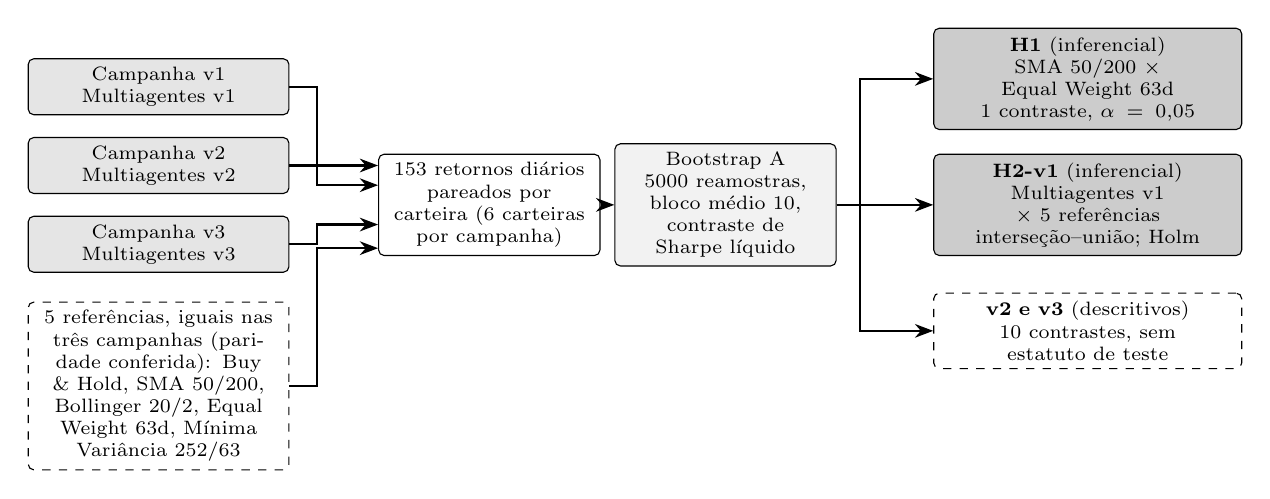
\begin{tikzpicture}[
  bx/.style={draw, rounded corners=2pt, align=center, font=\scriptsize, inner sep=3pt, text width=#1},
  bx/.default=3cm,
  arr/.style={-{Stealth}, thick},
]
\node[bx=3.1cm, fill=gray!20] (v1) at (0,1.5) {Campanha v1\\Multiagentes v1};
\node[bx=3.1cm, fill=gray!20] (v2) at (0,0.5) {Campanha v2\\Multiagentes v2};
\node[bx=3.1cm, fill=gray!20] (v3) at (0,-0.5) {Campanha v3\\Multiagentes v3};
\node[bx=3.1cm, dashed] (ref) at (0,-2.3) {5 referências, iguais nas três campanhas (paridade conferida): Buy \& Hold, SMA 50/200, Bollinger 20/2, Equal Weight 63d, Mínima Variância 252/63};
\node[bx=2.6cm] (ser) at (4.2,0) {153 retornos diários pareados por carteira (6 carteiras por campanha)};
\node[bx=2.6cm, fill=gray!10] (boot) at (7.2,0) {Bootstrap A\\5000 reamostras, bloco médio 10, contraste de Sharpe líquido};
\node[bx=3.7cm, fill=gray!40] (h1) at (11.8,1.6) {\textbf{H1} (inferencial)\\SMA 50/200 $\times$ Equal Weight 63d\\1 contraste, $\alpha = 0{,}05$};
\node[bx=3.7cm, fill=gray!40] (h2) at (11.8,0) {\textbf{H2-v1} (inferencial)\\Multiagentes v1 $\times$ 5 referências\\interseção--união; Holm};
\node[bx=3.7cm, dashed] (h3) at (11.8,-1.6) {\textbf{v2 e v3} (descritivos)\\10 contrastes, sem estatuto de teste};
\draw[arr] (v1.east) -- ++(0.35,0) |- ([yshift=0.25cm]ser.west);
\draw[arr] (v2.east) -- (v2.east -| ser.west);
\draw[arr] (v3.east) -- ++(0.35,0) |- ([yshift=-0.25cm]ser.west);
\draw[arr] (ref.east) -- ++(0.35,0) |- ([yshift=-0.55cm]ser.west);
\draw[arr] (ser) -- (boot);
\draw[arr] (boot.east) -- ++(0.3,0) |- (h1.west);
\draw[arr] (boot.east) -- (h2.west);
\draw[arr] (boot.east) -- ++(0.3,0) |- (h3.west);
\end{tikzpicture}
\caption{Desenho experimental do replay: três campanhas com seis carteiras cada, série pareada de 153 retornos, Bootstrap A e famílias de contrastes. Contornos tracejados indicam o que não recebe decisão inferencial.}
\label{fig:met-desenho}
{\footnotesize Fonte: elaborado pelos autores.}
\end{figure}

Na Figura~\ref{fig:met-desenho}, apenas H1 e H2-v1, cujas carteiras têm regras fixadas antes do replay, produzem decisão sobre H0; os contrastes de v2 e v3 usam o mesmo procedimento, mas são apenas descritivos.

\section{Operacionalização das Hipóteses}
\label{sec:met-hipoteses}

As hipóteses são as do Capítulo~\ref{cha:introducao}, preservadas do TCC 1:

\begin{itemize}
    \item \textbf{H1:} Estratégias baseadas em \textit{momentum} e \textit{trend following} apresentam desempenho superior ao \textit{equal weight} em termos de Sharpe Ratio líquido;
    \item \textbf{H2:} O sistema multiagente baseado em LLMs apresenta desempenho superior ajustado ao risco em relação aos \textit{benchmarks} considerados, tendo o Sharpe Ratio líquido como critério principal e o Sortino Ratio, o \textit{Maximum Drawdown} e o \textit{turnover} como critérios complementares;
    \item \textbf{H0:} Não há diferença estatisticamente significativa entre as abordagens.
\end{itemize}

No replay, cada hipótese é convertida em contrastes entre Sharpes de carteiras pareadas, conforme a Tabela~\ref{tab:met-hipoteses}. Para um par de carteiras $(A, B)$, o contraste é

\begin{equation}
\Delta_{A,B} = S_A - S_B,
\label{eq:met-contraste}
\end{equation}

\noindent em que $S$ é o Sharpe Ratio líquido da Seção~\ref{sec:met-metricas}, com hipótese nula unilateral $\Delta_{A,B} \leq 0$ e alternativa $\Delta_{A,B} > 0$.

\begin{table}[htbp]
\centering
\caption{Operacionalização das hipóteses no Replay Contínuo Abril--Novembro de 2026.}
\label{tab:met-hipoteses}
\small
\begin{tabular}{>{\raggedright\arraybackslash}p{1.8cm} >{\raggedright\arraybackslash}p{4.2cm} >{\raggedright\arraybackslash}p{3.2cm} >{\raggedright\arraybackslash}p{4.4cm}}
\toprule
\textbf{Hipótese} & \textbf{Carteiras comparadas} & \textbf{Contraste} & \textbf{Estatuto} \\
\midrule
H1 & SMA 50/200 $\times$ Equal Weight 63d & $\Delta_{\text{SMA},\text{EW}}$ & Principal; um contraste, $\alpha = 0{,}05$ \\
H2 (v1) & Multiagentes v1 $\times$ cada uma das cinco referências & $\Delta_{\text{v1},k}$, $k = 1,\ldots,5$ & Principal; família de cinco contrastes, $\alpha = 0{,}05$ (interseção--união; Holm para conclusões parciais) \\
H2 (v2, v3) & Multiagentes v2 e v3 $\times$ cada uma das cinco referências & $\Delta_{\text{v2},k}$, $\Delta_{\text{v3},k}$ & Exploratório; apenas descritivo \\
H0 & Todas as anteriores & Não rejeição em cada família & Decidida pelo Bootstrap A (Seção~\ref{sec:met-inferencia}) \\
\bottomrule
\end{tabular}
\end{table}

\paragraph*{H1.} A hipótese é operacionalizada pela carteira de referência SMA 50/200, única regra de tendência entre as referências, contra a carteira Equal Weight 63d, que materializa a linha de base de pesos iguais. As duas são determinísticas, não chamam o modelo de linguagem e foram calculadas antes de qualquer inferência paga, com parâmetros fixados pela \mbox{DP-36} e pelas definições multiativos existentes, sem calibração pelo resultado. O contraste de H1, portanto, não é afetado pela possível contaminação do modelo nem pelo ajuste das versões v2 e v3. A correspondência entre H1 e esse par foi estabelecida na redação deste trabalho, após o replay; ela não resulta de seleção entre alternativas, porque nenhuma outra referência implementa uma regra de tendência (a Bollinger 20/2 é de reversão à média e a Mínima Variância é uma regra de alocação por risco). O alcance de H1 fica restrito a uma regra de tendência com uma parametrização, e não à família de estratégias de \textit{momentum} \citep{JegadeeshTitman1993, Moskowitz2012} (Seção~\ref{sec:met-ameacas}).

\paragraph*{H2.} A carteira Multiagentes é comparada com as cinco referências: Buy \& Hold, SMA 50/200, Bollinger 20/2, Equal Weight 63d e Mínima Variância 252/63. O Sharpe líquido é o critério primário e o único submetido a contraste inferencial; Sortino, \textit{Maximum Drawdown}, retorno, volatilidade, operações, custos e giro são critérios complementares, reportados de forma descritiva, sem contrastes adicionais.

\paragraph*{Papel distinto das versões.} A versão v1 é a execução pré-especificada: reproduz a arquitetura multiativos já em operação diária (Seção~\ref{sec:arq-operacao-diaria}), com comitês, risco, gestor, esquemas, quórum, vetos e \textit{prompts} inalterados, e com o único ajuste autorizado de natureza operacional (até duas tentativas de transporte por chamada lógica). Dois ensaios curtos anteriores, sobre subjanelas (06--17/04/2026, escolhida antes de medir retorno, e 20/04--05/05/2026, escolhida pela queda observada), usaram a mesma arquitetura e não autorizaram calibração de vendas, \textit{prompts} ou controles. As regras da v1 foram fixadas antes da observação de seu desempenho na trajetória contínua de 153 pregões, e é dela que provém a resposta principal a H2; os ensaios, porém, observaram desempenho em trechos desse período, e a v1 não é independente deles. A pré-especificação refere-se ao replay, e não ao mercado: a arquitetura foi desenvolvida em 2026, quando parte do período já havia transcorrido, e não há registro de ajuste a ele, mas também não há prova de que não tenha havido influência.

As versões v2 e v3 são iterações exploratórias, desenhadas após a auditoria das versões anteriores sobre os mesmos 153 pregões (Seção~\ref{sec:arq-evolucao}). Seus limiares e regras foram escolhidos com conhecimento do período, das falhas observadas na versão anterior e do desempenho das referências; a v3, em particular, foi desenhada quando já se sabia qual referência havia obtido o melhor resultado. Cada uma foi executada uma única vez, sem amostra de validação separada. Por isso, \textbf{os resultados de v2 e v3 são otimistas por construção}: a melhora em relação à v1 mede a capacidade da arquitetura de incorporar correções dentro da amostra, e não desempenho esperado fora dela. Seus contrastes com as referências são calculados pelo mesmo procedimento da v1 e reportados apenas como descrição, sem estatuto de teste. A comparação entre as versões responde à pergunta arquitetural da Seção~\ref{sec:met-caracterizacao} e atribui as diferenças ao conjunto de intervenções de cada versão, e não a mecanismos isolados.

\paragraph*{H0.} Na operacionalização, H0 é a hipótese nula unilateral $\Delta_{A,B} \leq 0$ de cada contraste, coerente com o enunciado de superioridade de H1 e H2. A hipótese nula é decidida separadamente em cada família pelo Bootstrap A. Para H1, H0 é rejeitada quando o contraste $\Delta_{\text{SMA},\text{EW}}$ atende ao critério de superioridade da Seção~\ref{sec:met-inferencia}. Para H2, o enunciado de superioridade em relação aos \textit{benchmarks} só é sustentado se os cinco contrastes da v1 atenderem ao critério; a superioridade em relação a referências individuais é declarada apenas após a correção de multiplicidade da Seção~\ref{sec:met-inferencia}. Contrastes de v2 e v3 não rejeitam H0, qualquer que seja seu valor-$p$. A não rejeição de H0 não demonstra igualdade de desempenho: em uma amostra de 153 pregões, ela é compatível com diferenças econômicas relevantes que o teste não tem poder para detectar.

\section{Carteiras de Referência}
\label{sec:met-referencias}

As cinco referências são determinísticas, não chamam modelos e reutilizam implementações existentes do repositório, com os mesmos preços, custo, planejador de execução e livro da carteira Multiagentes (Seção~\ref{sec:arq-replay}). A Tabela~\ref{tab:met-referencias} resume suas regras e o papel de cada uma no estudo. Todas partem da cesta inicial imposta, operam somente posições compradas, sem alavancagem, e mantêm os proventos em caixa, sem reinvestimento. Os sinais de SMA e Bollinger são calculados sobre o fechamento B3 multiplicado pelo fator de ajuste congelado no \textit{bundle} da campanha, com decisão no fechamento de um pregão e execução na abertura do pregão seguinte; as operações e o patrimônio usam preços RAW B3.

\begin{table}[htbp]
\centering
\caption{Carteiras de referência do Replay Contínuo e seu papel no estudo.}
\label{tab:met-referencias}
\small
\begin{tabular}{>{\raggedright\arraybackslash}p{2.6cm} >{\raggedright\arraybackslash}p{8.4cm} >{\raggedright\arraybackslash}p{3.2cm}}
\toprule
\textbf{Carteira} & \textbf{Regra} & \textbf{Papel} \\
\midrule
Buy \& Hold & Mantém a cesta inicial, sem rebalanceamento (\mbox{DP-11}). & H2 \\
SMA 50/200 & Por ativo, parcela independente de 20\% do capital inicial; vende a posição inteira no cruzamento descendente da média de 50 pregões sob a de 200 e recompra, com o saldo da própria parcela, no cruzamento ascendente, apenas se a posição estiver zerada (\texttt{sma\_cross.py}, \mbox{DP-36}). & H1 (tendência); H2 \\
Bollinger 20/2 & Mesma mecânica de parcelas; compra no rompimento da banda inferior (20 pregões, 2 desvios) com posição zerada e vende a posição inteira no rompimento da banda superior (\texttt{bollinger\_bands.py}, \mbox{DP-36}). & H2 \\
Equal Weight 63d & Rebalanceia para pesos iguais (1/5) na primeira sessão e a cada 63 pregões (\texttt{EqualWeightPortfolio}). & H1 (linha de base); H2 \\
Mínima Variância 252/63 & Pesos de mínima variância estimados com 252 retornos, somente comprados, recalculados na primeira sessão e a cada 63 pregões (\texttt{MinVariancePortfolio}, SLSQP com objetivo reescalado). & H2 \\
\bottomrule
\end{tabular}
\end{table}

Três propriedades dessas regras são relevantes para a interpretação. Primeiro, a SMA 50/200 é uma regra de eventos: partindo da cesta já investida, ela só altera a posição de um ativo quando ocorre um cruzamento de médias, de modo que, em um período sem cruzamentos, sua trajetória coincide com a do Buy \& Hold naquele ativo, possibilidade aceita explicitamente na \mbox{DP-36}. Segundo, como a cesta inicial já tem pesos próximos de 20\%, a Equal Weight 63d difere do Buy \& Hold apenas pelos três rebalanceamentos do período, decididos nos fechamentos das sessões 1, 64 e 127 e executados na abertura seguinte. Terceiro, a carteira de pesos iguais é um referencial reconhecidamente difícil de superar em alocação de carteiras \citep{DeMiguel2009}, o que torna o contraste de H1 exigente. O primeiro sinal das referências usa o fechamento do primeiro pregão da campanha, enquanto a primeira decisão dos agentes usa o fechamento anterior; essa assimetria de uma sessão decorre da \mbox{DP-36} e é registrada no manifesto da campanha.

\section{Métricas de Avaliação}
\label{sec:met-metricas}

As métricas são calculadas sobre a série de 153 retornos diários $r_1, \ldots, r_n$ ($n = 153$) e sobre a curva de patrimônio da Seção~\ref{sec:met-desenho}, com as funções de \texttt{src/backtesting/metrics.py}. O cálculo para o replay está em \path{tcc2/scripts/metricas_replay.py}, que confere, por asserções, os estados diários, a paridade das referências entre versões e os totais de patrimônio, operações e custos contra os documentos de auditoria.

\paragraph*{Sharpe Ratio líquido (critério primário).} Adota-se a definição congelada \texttt{H2\_SCIENTIFIC\_SHARPE\_DEFINITION\_V1}:

\begin{equation}
S = \frac{\bar{r} - r_f/252}{\hat{\sigma}_r}\,\sqrt{252}, \qquad r_f = 0,
\label{eq:met-sharpe}
\end{equation}

\noindent em que $\bar{r}$ é a média dos retornos diários líquidos e $\hat{\sigma}_r$ seu desvio-padrão amostral (\textit{ddof} = 1). Quando há menos de dois retornos ou o desvio-padrão é nulo, inferior a $10^{-15}$ ou não numérico, a convenção do protocolo atribui $S = 0$; dados inválidos interrompem o cálculo. A definição foi congelada para o protocolo da Seção~\ref{sec:met-protocolo} e é reutilizada no replay para manter a mesma fórmula. A taxa livre de risco nula é coerente com a contabilidade da simulação, na qual o caixa não é remunerado, mas ignora o custo de oportunidade de uma taxa de juros positiva.

\paragraph*{Sortino Ratio.} No replay, a função \texttt{sortino\_ratio} usa a taxa livre de risco anual $r_f = 0$ e o retorno mínimo aceitável diário $\text{MAR} = 0$ para calcular o índice anualizado pela seguinte expressão.

\begin{equation}
\text{Sortino} = \frac{\bar{r} - r_f/252}{\sqrt{\frac{1}{n}\sum_{t=1}^{n}\min(r_t - \text{MAR}, 0)^2}}\,\sqrt{252}.
\label{eq:met-sortino}
\end{equation}

\noindent Na definição de \citet{Sortino1994}, o numerador é o retorno médio menos o MAR. No replay, $r_f/252 = \text{MAR} = 0$, de modo que os numeradores coincidem. O desvio de queda calculado a partir dos retornos diários e o fator de anualização $\sqrt{252}$ são convenções da implementação. Esses parâmetros são valores técnicos do módulo, não política científica congelada.

\paragraph*{\textit{Maximum Drawdown}.} Maior queda relativa entre um pico e um vale posterior da curva de patrimônio \citep{Magdon2004}, calculada por \texttt{max\_drawdown}, acompanhada da maior sequência de pregões consecutivos abaixo do pico anterior (\texttt{max\_drawdown\_duration}).

\paragraph*{Retorno e volatilidade.} Retorno total no período, retorno anualizado composto (expoente $252/153$) e volatilidade anualizada (desvio amostral $\times\sqrt{252}$). A anualização de 153 pregões é extrapolação e serve apenas para comparar escalas.

\paragraph*{Operações, custos e giro.} As operações são contadas como mudanças de quantidade de um ativo entre estados diários consecutivos, a partir da cesta inicial, cuja montagem não entra na contagem. O custo é o total acumulado de custos de negociação. Como o custo é proporcional e único (0,03\%), o volume negociado é estimado por $V = C / 0{,}0003$, e o giro no período é

\begin{equation}
\text{Giro} = \frac{C / 0{,}0003}{\overline{PL}},
\label{eq:met-giro}
\end{equation}

\noindent em que $C$ é o custo total e $\overline{PL}$ o patrimônio médio dos 153 fechamentos. O arredondamento do custo ao centavo admite erro de até cerca de R\$~16,67 no volume estimado de cada operação. Essa medida de \textit{turnover} difere da função \texttt{turnover} de \texttt{metrics.py}, que mede a variação de pesos, e da definição do protocolo original (nocional executado sobre o capital inicial); é a medida adotada no replay porque é reconstruível diretamente das séries seladas.

\section{Inferência Estatística}
\label{sec:met-inferencia}

\subsection{Bootstrap A}

A decisão sobre H0 utiliza o procedimento denominado Bootstrap A, especificado no protocolo original e implementado em \texttt{src/experiments/h2\_evaluation.py}: \textit{bootstrap} estacionário temporal pareado, na forma básica centrada. Para cada contraste $\Delta_{A,B}$ da Equação~\eqref{eq:met-contraste}:

\begin{enumerate}
    \item as séries de retornos diários de $A$ e $B$ são alinhadas nas mesmas 153 sessões; perda, divergência ou reordenação de sessões interrompe o cálculo, sem junção parcial nem preenchimento;
    \item calcula-se a estimativa pontual $\hat{\Delta} = S_A - S_B$ pela Equação~\eqref{eq:met-sharpe};
    \item geram-se $B = 5000$ sequências de índices de tamanho $n$ pelo \textit{bootstrap} estacionário, com gerador NumPy PCG64 e semente 20261008: o primeiro índice é sorteado uniformemente e, a cada passo, com probabilidade $1/10$ inicia-se um novo bloco em posição uniforme ou, caso contrário, avança-se para o índice seguinte, de forma circular; o comprimento médio dos blocos é, portanto, 10 pregões;
    \item a mesma sequência de índices reamostra as duas séries, o que preserva a dependência serial dentro dos blocos e a correlação contemporânea entre as carteiras;
    \item em cada reamostra $b$, recalcula-se $\hat{\Delta}^{*}_{b}$ e o erro centrado $e_b = \hat{\Delta}^{*}_{b} - \hat{\Delta}$;
    \item o valor-$p$ unilateral e o limite inferior unilateral de 95\% são
    \begin{equation}
    p_{+} = \frac{1 + \#\{b : e_b \geq \hat{\Delta}\}}{B + 1}, \qquad L_{95} = \hat{\Delta} - e_{(4751)},
    \label{eq:met-bootstrap}
    \end{equation}
    em que $e_{(4751)}$ é a 4751.ª estatística de ordem dos erros, sem interpolação;
    \item a superioridade de $A$ sobre $B$ exige estimabilidade, $\hat{\Delta} > 0$, $p_{+} < \alpha$ e $L_{95} > 0$. Se a série original ou alguma reamostra for degenerada (Sharpe atribuído por convenção) ou se todos os erros forem iguais, o resultado é inconclusivo, sem exclusão nem repetição de reamostras.
\end{enumerate}

A reamostragem por blocos de comprimento geométrico segue o \textit{bootstrap} estacionário de \citet{Politis1994}.

O protocolo original define o estimador como a média dos Sharpes de três execuções independentes do modelo menos o Sharpe do Buy \& Hold. No replay há uma execução por versão. A aplicação (\texttt{tcc2/scripts/bootstrap\_replay.py}) reutiliza sem alteração a função \texttt{bootstrap} de \texttt{h2\_evaluation.py}: a carteira $B$ ocupa a posição do Buy \& Hold e a carteira $A$ é repetida nas três posições das execuções do modelo, de modo que o estimador se reduz a $\hat{\Delta} = S_A - S_B$, enquanto a reamostragem, a semente, o número de reamostras, o bloco médio, o posto e a regra de decisão permanecem os do protocolo; todas as comparações usam a mesma sequência de índices. Como complemento descritivo, fora da regra de decisão, a função é aplicada também com os papéis invertidos, o que fornece um valor-$p$ unilateral de inferioridade e o limite superior $U_{95} = \hat{\Delta} - e_{(250)}$; o intervalo $[L_{95}; U_{95}]$ corresponde a um intervalo bilateral de 90\%. Duas consequências decorrem dessa adaptação. A inferência é condicional à única trajetória observada do modelo: ela trata a variabilidade temporal dos retornos, mas não a variabilidade entre execuções de um modelo estocástico com temperatura 1,0, que não pode ser estimada sem repetições. Além disso, o poder é baixo: sob retornos independentes, o erro-padrão aproximado de um Sharpe anualizado estimado com $n$ retornos diários é da ordem de $\sqrt{252/n}$ \citep{Lo2002}, cerca de 1,3 para $n = 153$; o pareamento reduz a variância do contraste quando as carteiras são correlacionadas, mas diferenças de Sharpe moderadas permanecem indistinguíveis de ruído amostral nessa janela. As limitações declaradas no protocolo também se aplicam: o \textit{bootstrap} básico não studentizado depende de estacionariedade aproximada e de dependência fraca, e o bloco médio de 10 não tem otimalidade demonstrada.

\subsection{Multiplicidade}

Os contrastes são organizados em famílias, e apenas as famílias principais da Tabela~\ref{tab:met-hipoteses}, cujas carteiras têm regras fixadas antes do replay, recebem decisão inferencial:

\begin{itemize}
    \item \textbf{H1:} um único contraste ($\Delta_{\text{SMA},\text{EW}}$), decidido com $\alpha = 0{,}05$;
    \item \textbf{H2:} cinco contrastes da v1 contra as referências. O protocolo original previa um único contraste confirmatório, contra o Buy \& Hold; no replay, a comparação se estende às cinco referências. O enunciado de H2, de superioridade em relação ao conjunto dos \textit{benchmarks}, corresponde a um teste de interseção--união: exige que os cinco contrastes atendam, cada um, à regra de superioridade com $\alpha = 0{,}05$, e por isso dispensa correção. A afirmação de superioridade em relação a referências individuais, quando nem todas forem superadas, exige controle do erro de tipo I da família; para ela, os valores $p_{+}$ são ajustados pelo método de \citet{Holm1979} dentro da família de cinco contrastes, e a superioridade parcial exige $p_{+}$ ajustado inferior a 0,05, além de $\hat{\Delta} > 0$ e $L_{95} > 0$;
    \item \textbf{v2 e v3:} os dez contrastes adicionais e as comparações entre versões não compõem família inferencial. Seus valores-$p$, inclusive os ajustados por Holm, são reportados apenas para descrição; nenhum ajuste corrige a busca implícita que gerou as versões, e, como as regras foram escolhidas com base nos mesmos dados, um valor-$p$ inferior a 0,05 nessas versões não tem interpretação de teste nem rejeita H0 \citep{White2000, Bailey2017}.
\end{itemize}

\section{Acompanhamento Prospectivo}
\label{sec:met-prospectivo}

A avaliação compatível com a \mbox{DP-31} é o acompanhamento diário prospectivo da carteira multiativos, iniciado em 14/10/2026 com carteiras Multiagentes e Buy \& Hold de mesma cesta inicial (\mbox{DP-20}), com a arquitetura da v1 (as regras da v2 e da v3 existem apenas nos \textit{scripts} do replay), e conduzido pelo ciclo autônomo descrito na Seção~\ref{sec:arq-operacao-diaria}. Nesse regime, cada decisão é registrada antes de o desfecho existir, o que exclui por construção a contaminação do modelo pelo resultado. O acompanhamento é a continuação natural do replay, mas, no horizonte deste trabalho, cobre poucas semanas e não sustenta inferência sobre as hipóteses; sua observação preliminar é apresentada no Capítulo~\ref{cha:resultados} (Seção~\ref{sec:obs-operacional}). A avaliação prospectiva da v3 com regras congeladas, sem novos ajustes, é trabalho futuro e o passo que poderia converter os achados exploratórios da v2 e da v3 em evidência fora da amostra.

\section{Ameaças à Validade}
\label{sec:met-ameacas}

\paragraph*{Contaminação do modelo e antecipação de informação.} Os controles de causalidade garantem que nenhuma entrada entregue aos agentes contenha informação posterior à sessão de referência (Seção~\ref{sec:arq-relogio}), mas não impedem que o modelo conheça o período por seu treinamento. O corte de conhecimento declarado do \texttt{gemini-3.8-flash} (março de 2026) antecede o período, mas não é verificável: o corpus de treinamento não é auditável, as campanhas foram executadas em 13, 15 e 16/11/2026, depois do período, e o identificador do modelo é um \textit{alias} sem garantia de versão imutável. Os analistas técnicos e o analista de risco recebem apenas \textit{features} adimensionais e métricas de risco, sem \textit{ticker}, data nem preço, o que fecha nessas etapas o canal de memorização do período; o gestor, porém, recebe \textit{tickers}, datas e preços, e é o canal exposto. Não houve anonimização dos ativos no gestor nem teste de detecção de contaminação, estratégias discutidas na Seção~\ref{sec:rel-avaliacao} \citep{Glasserman2023, Golchin2024, Drinkall2024}. Além disso, preços, fatores de ajuste e proventos foram adquiridos depois do período e não constituem um arquivo \textit{point-in-time}. A contaminação, se existir, tende a favorecer a carteira Multiagentes: em agentes LLM de negociação, retornos de \textit{backtest} obtidos dentro da janela de conhecimento do modelo desaparecem fora dela \citep{ProfitMirage2025}, e conhecer apenas o \textit{ticker} e a data já permite algum acerto direcional antes do corte \citep{Wang2026}. O efeito não é garantido, pois o conhecimento prévio sobre a empresa também pode prejudicar a decisão \citep{Glasserman2023}. A contaminação não afeta as referências determinísticas nem, portanto, o contraste de H1.

\paragraph*{Ajuste dentro da amostra.} As versões v2 e v3 foram desenhadas após a observação das versões anteriores nos mesmos 153 pregões, com limiares escolhidos com conhecimento do período e das referências, e sem amostra de validação. Seus resultados são otimistas por construção e podem refletir sobreajuste a esta trajetória \citep{White2000, Bailey2017}. A resposta principal a H2 limita-se, por isso, à v1.

\paragraph*{Amostra única e escopo reduzido.} O estudo cobre uma única trajetória de 153 pregões, cinco ações do mercado brasileiro e um único regime de mercado. Cada versão foi executada uma vez, sem repetições que permitam estimar a variância entre execuções do modelo. O poder estatístico é baixo (Seção~\ref{sec:met-inferencia}), e a ordenação das carteiras pode depender do regime do período; a validade externa é correspondentemente limitada.

\paragraph*{Intervenções em bloco.} Cada versão alterou vários fatores ao mesmo tempo (Tabela~\ref{tab:evolucao-versoes}), sem ablação. Não é possível atribuir efeito a cada pilar isoladamente, e parte dos mecanismos pode não ter sido acionada no período. Também diferem entre as versões o número de pregões sem análise e, possivelmente, a versão do modelo servida sob o mesmo \textit{alias} em cada data de execução, fatores de confusão que o desenho não elimina.

\paragraph*{Custo e execução simplificados.} A execução usa a abertura oficial diária (PREABE) como aproximação do leilão, sem \textit{spread}, impacto de mercado, microestrutura ou liquidação em D+2, e com aprovação hipotética às 09:00. O custo é proporcional (0,03\%), sem custo fixo nem lote mínimo, o que favorece estratégias com muitas operações pequenas. O custo de inferência não é deduzido do patrimônio da carteira Multiagentes. O JCP é creditado líquido de 15\% de imposto, mas não há imposto sobre ganho de capital, assimetria que favorece estratégias que realizam lucros. A ausência de remuneração do caixa não é neutra: penaliza as carteiras com mais caixa médio (Bollinger 20/2, 49,06\%, e SMA 50/200, 31,39\%) em relação às sempre investidas (Buy \& Hold, Equal Weight 63d e Mínima Variância 252/63, todas com caixa médio inferior a 1\%). Para dimensionar, o CDI acumulado no período foi de 8,33\% \citep{BCBCDI2026}. A diferença de caixa médio entre a SMA 50/200 e a Equal Weight 63d é de 30,69 pontos percentuais, e a remuneração desse excedente ao CDI daria, em aproximação que ignora o momento em que o caixa esteve aplicado, cerca de 2,56 pontos percentuais ($30{,}69\% \times 8{,}33\%$), contra uma diferença de retorno de 1,00 ponto percentual a favor da Equal Weight 63d ($-11{,}13\%$ contra $-10{,}13\%$). Nenhuma carteira superou o CDI do período; a maior, a Bollinger 20/2, rendeu 4,89\%. O contraste de Sharpe de H1, calculado com $r_f = 0$, deve ser lido com essa ressalva.

\paragraph*{Cesta inicial imposta.} Todas as carteiras partem da mesma cesta investida, montada a custo zero. Essa condição torna a comparação pareada, mas condiciona os resultados: a Equal Weight 63d permanece próxima do Buy \& Hold, a SMA 50/200 só se afasta da cesta inicial quando ocorrem cruzamentos, e a carteira Multiagentes não escolhe sua alocação de partida.

\paragraph*{Alcance de H1.} H1 é respondida por uma única regra de tendência, a SMA 50/200 em sua forma de eventos com parcelas independentes por ativo, contra uma carteira de pesos iguais com rebalanceamento a cada 63 pregões. O resultado não se generaliza para a família de estratégias de \textit{momentum} e \textit{trend following}, que inclui o \textit{momentum} transversal \citep{JegadeeshTitman1993}, o \textit{momentum} de série temporal \citep{Moskowitz2012}, outras regras de médias móveis \citep{Brock1992} e outras janelas e parametrizações.

\paragraph*{Síntese.} A Tabela~\ref{tab:met-ameacas} resume o sentido provável do viés de cada ameaça e os resultados que ela alcança; ela sintetiza os parágrafos acima e não os substitui.

\begin{table}[htbp]
\centering
\caption{Ameaças à validade, sentido provável do viés e resultados afetados.}
\label{tab:met-ameacas}
\small
\begin{tabular}{>{\raggedright\arraybackslash}p{3.6cm} >{\raggedright\arraybackslash}p{5.8cm} >{\raggedright\arraybackslash}p{4.6cm}}
\toprule
\textbf{Ameaça} & \textbf{Sentido provável do viés} & \textbf{Resultados afetados} \\
\midrule
Contaminação do modelo & Tende a favorecer a Multiagentes; não garantido; canal restrito ao gestor & v1, v2 e v3; não afeta H1 \\
Ajuste dentro da amostra & Favorece v2 e v3 & v2 e v3 \\
Execução única, temperatura 1,0 & Indeterminado & v1, v2 e v3 \\
Caixa sem remuneração (CDI de 8,33\% no período) & Penaliza carteiras com mais caixa médio (Bollinger 20/2, SMA 50/200) & H1 (descritivo); referências com caixa \\
Custo apenas proporcional (0,03\%) & Favorece muitas operações pequenas & Carteiras com mais operações \\
Sem imposto sobre ganho de capital & Favorece quem realiza lucro & Carteiras com vendas lucrativas \\
Cesta inicial imposta & Aproxima a Equal Weight 63d do Buy \& Hold e limita a SMA 50/200 & H1 \\
Seleção do universo & Indeterminado & Níveis de todas as carteiras \\
\bottomrule
\end{tabular}
\end{table}

Nenhum desempenho dos agentes é presumido a priori. Os resultados do replay são apresentados no Capítulo~\ref{cha:resultados} como evidência descritiva desta trajetória, com decisão inferencial restrita aos contrastes pré-especificados e sujeita às ameaças acima.

\chapter{Resultados e Discussão}
\label{cha:resultados}

% Fontes: tcc2/agent-reports/METRICAS_REPLAY.md e chapters/tabelas/metricas-replay.tex
% (scripts/metricas_replay.py); tcc2/agent-reports/BOOTSTRAP_REPLAY.md e
% chapters/tabelas/bootstrap-replay.tex (scripts/bootstrap_replay.py);
% tcc2/evidence/04-replay-abril-novembro/relatorios/evolucao_replay_v1_v2_v3_tcc.md
% (documento mestre, seções 1.2, 2 a 6); auditoria_posicoes_replay_2026-04_2026-11.md;
% replay_continuo_v2_2026-04_2026-11.md; replay_continuo_v3_2026-04_2026-11.md;
% tcc2/evidence/Resultados-comparados.md; tcc2/evidence/01-direcao-e-estado/ESTADO_ATUAL.md.
Este capítulo apresenta os resultados do Replay Contínuo Abril--Novembro de 2026, obtidos sob o desenho descrito no Capítulo~\ref{cha:metodologia}: seis carteiras --- a carteira Multiagentes e cinco referências determinísticas --- percorrem os mesmos 153 pregões, a partir da mesma cesta inicial, em três campanhas sucessivas da carteira Multiagentes (v1, v2 e v3). A leitura dos resultados obedece à distinção estabelecida na Seção~\ref{sec:met-hipoteses}. Recebem decisão inferencial apenas o contraste de H1, entre duas referências determinísticas, e a família de contrastes de H2 na versão v1, cujas regras foram fixadas antes do replay. As versões v2 e v3 foram desenhadas após a observação do mesmo período e são exploratórias: seus contrastes são calculados pelo mesmo procedimento, mas reportados apenas como descrição, e nenhum valor-$p$ obtido nelas rejeita H0. Todos os números referem-se a uma única trajetória de mercado e são, portanto, resultados dentro da amostra.

O capítulo está organizado em seis partes: o contexto de mercado do período (Seção~\ref{sec:res-mercado}); os resultados agregados das seis carteiras nas três versões (Seção~\ref{sec:res-agregados}); a decisão sobre as hipóteses (Seção~\ref{sec:res-hipoteses}); a evolução arquitetural entre as versões, que responde à pergunta secundária do estudo (Seção~\ref{sec:res-evolucao}); a discussão do alcance dos resultados (Seção~\ref{sec:res-discussao}); e, separadamente, uma observação preliminar do acompanhamento prospectivo, que não integra o replay (Seção~\ref{sec:obs-operacional}).

\section{Contexto de Mercado do Período}
\label{sec:res-mercado}

A Tabela~\ref{tab:res-mercado} compara, para cada ativo do universo, o preço de referência da cesta inicial (fechamento de 02/04/2026) com o fechamento do último pregão do replay (12/11/2026). Quatro dos cinco ativos caíram no período, com perdas expressivas em BBAS3 e VALE3; apenas WEGE3 encerrou acima do preço de entrada. As variações são somente de preço e não incluem proventos.

\begin{table}[htbp]
\centering
\caption{Variação de preço dos ativos do universo no período do Replay Contínuo (preço de referência de entrada em 02/04 e fechamento em 12/11).}
\label{tab:res-mercado}
\small
\begin{tabular}{lrrr}
\toprule
\textbf{Ativo} & \textbf{02/04 (R\$)} & \textbf{12/11 (R\$)} & \textbf{Var. (\%)} \\
\midrule
BBAS3 & 23{,}39 & 15{,}48 & $-33{,}82$ \\
VALE3 & 83{,}55 & 63{,}95 & $-23{,}46$ \\
PETR4 & 48{,}15 & 44{,}70 & $-7{,}17$ \\
ITUB4 & 43{,}30 & 41{,}68 & $-3{,}74$ \\
WEGE3 & 50{,}31 & 51{,}65 & $+2{,}66$ \\
\bottomrule
\end{tabular}
\par\smallskip\footnotesize Fonte: documento mestre do replay (\texttt{evolucao\_replay\_v1\_v2\_v3\_tcc.md}, Seção 1.2), a partir de \texttt{operacoes\_v3.csv} e dos relatórios de auditoria.
\end{table}

Como a cesta inicial imposta tem pesos próximos de 20\% por ativo (Seção~\ref{sec:met-desenho}), esse movimento define o ponto de partida comum: a carteira Buy \& Hold, que apenas mantém a cesta, perdeu 11,21\% no período. Além da tendência de queda, a trajetória inclui um recuo concentrado no fim de outubro, visível nas curvas de \textit{drawdown} das carteiras que permaneceram investidas (Figura~\ref{fig:replay-drawdown}). Esse regime de queda condiciona a comparação entre as carteiras, ponto retomado na Seção~\ref{sec:res-discussao}.

\section{Resultados Agregados das Carteiras}
\label{sec:res-agregados}

As Tabelas~\ref{tab:replay-risco} e~\ref{tab:replay-operacoes} reúnem as métricas da Seção~\ref{sec:met-metricas} para as três versões da carteira Multiagentes e para as cinco referências, que são idênticas nas três campanhas, conforme a auditoria de paridade (Seção~\ref{sec:arq-replay}). As Figuras~\ref{fig:replay-patrimonio} e~\ref{fig:replay-drawdown} mostram as curvas de patrimônio e de \textit{drawdown}.

% Gerado por tcc2/scripts/metricas_replay.py; não editar à mão.
\begin{table}[htbp]
\centering
\caption{Retorno e risco das carteiras no Replay Contínuo, 06/04/2026 a 12/11/2026 (153 pregões). Sharpe pela definição \texttt{H2\_SCIENTIFIC\_SHARPE\_DEFINITION\_V1} ($r_f = 0$); Sortino com $r_f = 0$ e MAR $= 0$.}
\label{tab:replay-risco}
\small
\setlength{\tabcolsep}{4pt}
\resizebox{\textwidth}{!}{%
\begin{tabular}{lrrrrrrc}
\toprule
Carteira & Retorno (\%) & Ret. anual. (\%) & Vol. anual. (\%) & Sharpe & Sortino & MDD (\%) & Pico--vale \\
\midrule
Multiagentes v1 & $-17{,}82$ & $-27{,}62$ & 23{,}17 & $-1{,}28$ & $-1{,}60$ & $-22{,}90$ & 14/04--12/08 \\
Multiagentes v2 & $-14{,}26$ & $-22{,}38$ & 19{,}33 & $-1{,}21$ & $-1{,}58$ & $-19{,}37$ & 14/04--06/11 \\
Multiagentes v3 & 0{,}07 & 0{,}11 & 16{,}01 & 0{,}09 & 0{,}13 & $-12{,}80$ & 14/04--10/06 \\
\midrule
Buy \& Hold & $-11{,}21$ & $-17{,}78$ & 22{,}08 & $-0{,}78$ & $-1{,}01$ & $-18{,}53$ & 05/10--05/11 \\
SMA 50/200 & $-11{,}13$ & $-17{,}67$ & 13{,}11 & $-1{,}42$ & $-1{,}77$ & $-16{,}61$ & 14/04--06/11 \\
Bollinger 20/2 & 4{,}89 & 8{,}18 & 11{,}77 & 0{,}73 & 1{,}16 & $-8{,}52$ & 30/04--05/06 \\
Equal Weight 63d & $-10{,}13$ & $-16{,}13$ & 21{,}61 & $-0{,}71$ & $-0{,}94$ & $-18{,}10$ & 05/10--05/11 \\
Mínima Variância 252/63 & $-4{,}19$ & $-6{,}80$ & 17{,}52 & $-0{,}32$ & $-0{,}47$ & $-14{,}95$ & 13/04--05/06 \\
\bottomrule
\end{tabular}}
\par\smallskip\footnotesize Fonte: \texttt{daily.csv} das campanhas \texttt{REPLAY-01} a \texttt{REPLAY-03}; 153 pregões, dentro da amostra.
\end{table}

\begin{table}[htbp]
\centering
\caption{Operações, custos e caixa das carteiras no Replay Contínuo. Giro = volume negociado estimado (custo / 0{,}03\%) dividido pelo patrimônio médio.}
\label{tab:replay-operacoes}
\small
\resizebox{\textwidth}{!}{%
\begin{tabular}{lrrrrrr}
\toprule
Carteira & Patrimônio final (R\$) & Operações (C/V) & Custos (R\$) & Giro & Caixa médio (\%) & Caixa final (\%) \\
\midrule
Multiagentes v1 & 82.178{,}71 & 86 (50/36) & 184{,}40 & 6{,}78 & 12{,}98 & 1{,}64 \\
Multiagentes v2 & 85.743{,}57 & 38 (22/16) & 119{,}87 & 4{,}34 & 24{,}69 & 45{,}86 \\
Multiagentes v3 & 100.067{,}36 & 81 (29/52) & 120{,}07 & 4{,}03 & 14{,}94 & 0{,}75 \\
\midrule
Buy \& Hold & 88.791{,}11 & 0 (0/0) & 0{,}00 & 0{,}00 & 0{,}70 & 1{,}60 \\
SMA 50/200 & 88.866{,}68 & 6 (2/4) & 32{,}23 & 1{,}16 & 31{,}39 & 39{,}29 \\
Bollinger 20/2 & 104.887{,}05 & 24 (12/12) & 151{,}26 & 4{,}92 & 49{,}06 & 1{,}44 \\
Equal Weight 63d & 89.869{,}29 & 15 (9/6) & 5{,}11 & 0{,}18 & 0{,}70 & 1{,}58 \\
Mínima Variância 252/63 & 95.814{,}84 & 14 (8/6) & 27{,}94 & 0{,}97 & 0{,}78 & 1{,}65 \\
\bottomrule
\end{tabular}}
\par\smallskip\footnotesize Fonte: \texttt{daily.csv} das campanhas \texttt{REPLAY-01} a \texttt{REPLAY-03}; 153 pregões, dentro da amostra.
\end{table}


% Gerado por tcc2/scripts/metricas_replay.py; requer \usepackage{pgfplots}.
\begin{figure}[htbp]
\centering
\begin{tikzpicture}
\begin{axis}[
  width=\textwidth, height=7.5cm, xmin=0, xmax=153,
  xtick={0,19,39,60,83,104,125,146},
  xticklabels={abr,mai,jun,jul,ago,set,out,nov},
  xlabel={Pregão (2026)}, ylabel={Patrimônio (R\$ mil)},
  ymajorgrids, grid style={gray!20}, tick label style={font=\footnotesize},
  label style={font=\small}, scaled y ticks=false,
  yticklabel style={/pgf/number format/use comma, /pgf/number format/1000 sep={.}},
  legend style={at={(0.5,-0.2)}, anchor=north, legend columns=3,
    font=\footnotesize, draw=none, /tikz/every even column/.append style={column sep=6pt}},
  legend cell align=left,
]
\addplot[black, thick, densely dotted] table[x=idx, y=eq_ma_v1, col sep=comma] {figures/replay-series.csv};
\addlegendentry{Multiagentes v1}
\addplot[black, thick, dashed] table[x=idx, y=eq_ma_v2, col sep=comma] {figures/replay-series.csv};
\addlegendentry{Multiagentes v2}
\addplot[black, very thick] table[x=idx, y=eq_ma_v3, col sep=comma] {figures/replay-series.csv};
\addlegendentry{Multiagentes v3}
\addplot[gray, thin] table[x=idx, y=eq_bh, col sep=comma] {figures/replay-series.csv};
\addlegendentry{Buy \& Hold}
\addplot[gray, dashdotted] table[x=idx, y=eq_sma, col sep=comma] {figures/replay-series.csv};
\addlegendentry{SMA 50/200}
\addplot[gray, mark=square*, mark repeat=15, mark size=1.4pt] table[x=idx, y=eq_boll, col sep=comma] {figures/replay-series.csv};
\addlegendentry{Bollinger 20/2}
\addplot[gray, densely dashed, mark=o, mark repeat=15, mark size=1.6pt, mark options={solid}] table[x=idx, y=eq_ew, col sep=comma] {figures/replay-series.csv};
\addlegendentry{Equal Weight 63d}
\addplot[gray, mark=triangle*, mark repeat=15, mark size=1.8pt] table[x=idx, y=eq_mv, col sep=comma] {figures/replay-series.csv};
\addlegendentry{Mínima Variância 252/63}
\end{axis}
\end{tikzpicture}
\caption{Patrimônio de fechamento das carteiras no Replay Contínuo, de 02/04/2026 (R\$~100 mil) a 12/11/2026. As referências são idênticas nas três campanhas.}
\label{fig:replay-patrimonio}
\end{figure}


% Gerado por tcc2/scripts/metricas_replay.py; requer \usepackage{pgfplots}.
\begin{figure}[htbp]
\centering
\begin{tikzpicture}
\begin{axis}[
  width=\textwidth, height=7.5cm, xmin=0, xmax=153,
  xtick={0,19,39,60,83,104,125,146},
  xticklabels={abr,mai,jun,jul,ago,set,out,nov},
  xlabel={Pregão (2026)}, ylabel={Drawdown (\%)},
  ymajorgrids, grid style={gray!20}, tick label style={font=\footnotesize},
  label style={font=\small}, scaled y ticks=false,
  yticklabel style={/pgf/number format/use comma, /pgf/number format/1000 sep={.}},
  legend style={at={(0.5,-0.2)}, anchor=north, legend columns=3,
    font=\footnotesize, draw=none, /tikz/every even column/.append style={column sep=6pt}},
  legend cell align=left,
]
\addplot[black, thick, densely dotted] table[x=idx, y=dd_ma_v1, col sep=comma] {figures/replay-series.csv};
\addlegendentry{Multiagentes v1}
\addplot[black, thick, dashed] table[x=idx, y=dd_ma_v2, col sep=comma] {figures/replay-series.csv};
\addlegendentry{Multiagentes v2}
\addplot[black, very thick] table[x=idx, y=dd_ma_v3, col sep=comma] {figures/replay-series.csv};
\addlegendentry{Multiagentes v3}
\addplot[gray, thin] table[x=idx, y=dd_bh, col sep=comma] {figures/replay-series.csv};
\addlegendentry{Buy \& Hold}
\addplot[gray, dashdotted] table[x=idx, y=dd_sma, col sep=comma] {figures/replay-series.csv};
\addlegendentry{SMA 50/200}
\addplot[gray, mark=square*, mark repeat=15, mark size=1.4pt] table[x=idx, y=dd_boll, col sep=comma] {figures/replay-series.csv};
\addlegendentry{Bollinger 20/2}
\addplot[gray, densely dashed, mark=o, mark repeat=15, mark size=1.6pt, mark options={solid}] table[x=idx, y=dd_ew, col sep=comma] {figures/replay-series.csv};
\addlegendentry{Equal Weight 63d}
\addplot[gray, mark=triangle*, mark repeat=15, mark size=1.8pt] table[x=idx, y=dd_mv, col sep=comma] {figures/replay-series.csv};
\addlegendentry{Mínima Variância 252/63}
\end{axis}
\end{tikzpicture}
\caption{Drawdown (queda em relação ao pico anterior) das carteiras no Replay Contínuo.}
\label{fig:replay-drawdown}
\end{figure}


\paragraph*{Leitura das curvas.} As Figuras~\ref{fig:replay-patrimonio} e~\ref{fig:replay-drawdown} mostram o que as tabelas não mostram: o caminho. Todas as carteiras partem juntas, atingem um pico em meados de abril e recuam em seguida. A partir de junho, a v1 passa a ocupar a base do gráfico, com o mínimo em agosto (o vale de 12/08), e só se reaproxima das demais por pouco tempo, no início de outubro. A v3 separa-se do grupo formado por Buy \& Hold, SMA 50/200, Equal Weight 63d e Mínima Variância 252/63 em meados de junho e permanece acima dele até o fim, mas termina abaixo da Bollinger 20/2. No início de outubro várias carteiras chegam perto do pico anterior ou o recuperam, e todas recuam em seguida: o fim do período concentra o maior recuo de Buy \& Hold e Equal Weight 63d (Seção~\ref{sec:res-agregados}). Essa leitura é visual e serve apenas para localizar no tempo os resultados das tabelas.

\paragraph*{Patrimônio e retorno.} Ordenadas pelo patrimônio final, as carteiras ficaram assim: Bollinger 20/2 (R\$~104.887,05; +4,89\%), Multiagentes v3 (R\$~100.067,36; +0,07\%), Mínima Variância 252/63 (R\$~95.814,84; $-4{,}19\%$), Equal Weight 63d (R\$~89.869,29; $-10{,}13\%$), SMA 50/200 (R\$~88.866,68; $-11{,}13\%$), Buy \& Hold (R\$~88.791,11; $-11{,}21\%$), Multiagentes v2 (R\$~85.743,57; $-14{,}26\%$) e Multiagentes v1 (R\$~82.178,71; $-17{,}82\%$). As versões v1 e v2 terminaram abaixo das cinco referências; a v3 terminou acima de quatro delas e R\$~4.819,69 abaixo da Bollinger 20/2. Apenas a Bollinger 20/2 teve retorno claramente positivo (+4,89\%); a v3 terminou praticamente no zero a zero (+0,07\%). Ambas compram em fraqueza e vendem em força (Seção~\ref{sec:res-v3}).

\paragraph*{Sharpe e Sortino.} Somente a Bollinger 20/2 (0,73) e a v3 (0,09) tiveram Sharpe positivo. Sob retornos independentes, o erro-padrão aproximado de um Sharpe anualizado estimado com 153 retornos diários é de ao menos cerca de 1,3, valor que cresce com o próprio Sharpe \citep{Lo2002}, de modo que diferenças dessa ordem não se distinguem de ruído amostral nesta janela. Há ainda uma propriedade do índice que afeta a ordenação quando o retorno médio é negativo: como a média negativa é dividida pela volatilidade, uma carteira menos volátil recebe um Sharpe mais negativo para o mesmo retorno. É o caso da SMA 50/200, cujo retorno ($-11{,}13\%$) praticamente coincide com o do Buy \& Hold ($-11{,}21\%$), com volatilidade (13,11\% contra 22,08\%) e \textit{drawdown} máximo ($-16{,}61\%$ contra $-18{,}53\%$) menores, mas cujo Sharpe ($-1{,}42$) é o mais baixo entre as oito carteiras. O Sortino reproduz a mesma ordenação. Essa propriedade é retomada na decisão sobre H1 e H2 (Seção~\ref{sec:res-hipoteses}).

\paragraph*{\textit{Drawdown}.} A v1 teve o maior \textit{drawdown} máximo ($-22{,}90\%$, de 14/04 a 12/08), seguida da v2 ($-19{,}37\%$); a v3 ($-12{,}80\%$) ficou atrás apenas da Bollinger 20/2 ($-8{,}52\%$). Para Buy \& Hold e Equal Weight 63d, o máximo ocorreu entre 05/10 e 05/11, no recuo do fim do período. A v1, a v2 e a SMA 50/200 permaneceram 146 pregões consecutivos abaixo do pico anterior, isto é, praticamente todo o período a partir de meados de abril.

\paragraph*{Operações, custos e caixa.} A v1 foi a carteira mais ativa: 86 operações posteriores à entrada, R\$~184,40 de custos e giro de 6,78 vezes o patrimônio médio. A v2 reduziu as operações para 38 e a v3 realizou 81, com predominância de vendas (52 contra 29 compras). Entre as referências, a Bollinger 20/2 operou 24 vezes, com giro de 4,92, e a SMA 50/200 apenas 6, com quatro saídas totais. Os custos acumulados, no máximo R\$~184,40, são pequenos diante das diferenças de patrimônio entre as carteiras, da ordem de milhares de reais; as diferenças decorrem, portanto, das decisões, e não do custo proporcional de 0,03\%, que não inclui custo fixo nem lote mínimo (Seção~\ref{sec:met-ameacas}). O caixa distingue as estratégias: em média, a Bollinger 20/2 manteve 49,06\% do patrimônio em caixa e a SMA 50/200, 31,39\%; nas três versões da Multiagentes, o caixa médio ficou entre 12,98\% e 24,69\%. Buy \& Hold, Equal Weight 63d e Mínima Variância 252/63 permaneceram investidas (caixa médio inferior a 1\%).

\paragraph*{Pregões sem análise.} A v1 concluiu os 153 pregões com análise completa. A v2 teve um pregão \texttt{NO\_ANALYSIS} (26/06), por falha de transporte em uma chamada de risco, e a v3 teve quatro (01/07, 01/09, 01/10 e 02/10), por respostas do gestor recusadas na validação determinística. Nesses pregões as posições foram preservadas e marcadas normalmente, sem decisão fabricada (Seção~\ref{sec:arq-replay}).

\section{Decisão sobre as Hipóteses}
\label{sec:res-hipoteses}

A Tabela~\ref{tab:replay-bootstrap} apresenta os 16 contrastes de Sharpe calculados pelo Bootstrap A (Seção~\ref{sec:met-inferencia}): o contraste de H1, os cinco contrastes da família principal de H2 (v1) e os dez contrastes descritivos das versões v2 e v3. Todos foram estimáveis, nenhum teve reamostra degenerada e todos usaram a mesma sequência de índices. A coluna ``Critério?'' indica se a regra numérica de superioridade foi atendida em cada linha; ela equivale a rejeitar H0 apenas nas linhas de H1 e de H2 (v1), enquanto nas linhas de v2 e v3 é descritiva, sem interpretação de teste (Seção~\ref{sec:met-inferencia}).
% Gerado por tcc2/scripts/bootstrap_replay.py; não editar à mão.
\begin{table}[H]
\centering
\caption{Comparações pareadas de Sharpe no Replay Contínuo (153 pregões) pelo \textit{bootstrap} A: estacionário, \textit{basic} centrado, $B=5000$, semente 20261008, bloco médio 10. $\Delta$ = Sharpe(A) $-$ Sharpe(B), $r_f = 0$. $p_+$ e $L_{95}$: teste unilateral de superioridade (regra congelada); $U_{95}$ e $p_-$: direção inversa, exploratória. Holm dentro de cada família de cinco referências.}
\label{tab:replay-bootstrap}
\setlength{\tabcolsep}{4pt}
\resizebox{\textwidth}{!}{%
\begin{tabular}{llrrrrrrc}
\toprule
Hipótese & A vs B & $\Delta$ & $L_{95}$ & $U_{95}$ & $p_+$ & $p_+$ Holm & $p_-$ & Critério? \\
\midrule
H1 & SMA 50/200 vs Equal Weight 63d & $-0{,}71$ & $-1{,}75$ & 0{,}31 & 0{,}881 & 0{,}881 & 0{,}119 & não \\
\midrule
H2 (v1) & MA v1 vs Buy \& Hold & $-0{,}50$ & $-1{,}76$ & 0{,}93 & 0{,}728 & 1{,}000 & 0{,}272 & não \\
H2 (v1) & MA v1 vs SMA 50/200 & 0{,}14 & $-1{,}32$ & 1{,}76 & 0{,}432 & 1{,}000 & 0{,}568 & não \\
H2 (v1) & MA v1 vs Bollinger 20/2 & $-2{,}00$ & $-4{,}47$ & 0{,}41 & 0{,}917 & 1{,}000 & 0{,}084 & não \\
H2 (v1) & MA v1 vs Equal Weight 63d & $-0{,}57$ & $-1{,}88$ & 0{,}88 & 0{,}753 & 1{,}000 & 0{,}248 & não \\
H2 (v1) & MA v1 vs Mínima Variância 252/63 & $-0{,}96$ & $-2{,}27$ & 0{,}29 & 0{,}899 & 1{,}000 & 0{,}102 & não \\
\midrule
H2 (v2) & MA v2 vs Buy \& Hold & $-0{,}44$ & $-1{,}34$ & 0{,}83 & 0{,}714 & 1{,}000 & 0{,}286 & não \\
H2 (v2) & MA v2 vs SMA 50/200 & 0{,}20 & $-1{,}02$ & 1{,}69 & 0{,}347 & 1{,}000 & 0{,}653 & não \\
H2 (v2) & MA v2 vs Bollinger 20/2 & $-1{,}94$ & $-4{,}27$ & 0{,}31 & 0{,}917 & 1{,}000 & 0{,}083 & não \\
H2 (v2) & MA v2 vs Equal Weight 63d & $-0{,}51$ & $-1{,}46$ & 0{,}77 & 0{,}747 & 1{,}000 & 0{,}253 & não \\
H2 (v2) & MA v2 vs Mínima Variância 252/63 & $-0{,}90$ & $-1{,}96$ & 0{,}22 & 0{,}912 & 1{,}000 & 0{,}088 & não \\
\midrule
H2 (v3) & MA v3 vs Buy \& Hold & 0{,}86 & $-0{,}30$ & 2{,}13 & 0{,}108 & 0{,}432 & 0{,}892 & não \\
H2 (v3) & MA v3 vs SMA 50/200 & 1{,}50 & 0{,}25 & 3{,}02 & 0{,}024 & 0{,}121 & 0{,}976 & sim$^{*}$ \\
H2 (v3) & MA v3 vs Bollinger 20/2 & $-0{,}64$ & $-1{,}79$ & 0{,}59 & 0{,}812 & 0{,}812 & 0{,}188 & não \\
H2 (v3) & MA v3 vs Equal Weight 63d & 0{,}79 & $-0{,}34$ & 2{,}00 & 0{,}122 & 0{,}432 & 0{,}878 & não \\
H2 (v3) & MA v3 vs Mínima Variância 252/63 & 0{,}40 & $-1{,}09$ & 1{,}77 & 0{,}334 & 0{,}668 & 0{,}666 & não \\
\bottomrule
\end{tabular}}
\par\smallskip\footnotesize v1: execução pré-especificada; v2 e v3: iterações exploratórias desenhadas após observar o mesmo período (p-valores otimistas). Critério: $\hat{\Delta} > 0$, $p_+ < 0{,}05$ e $L_{95} > 0$; só rejeita $H_0$ em H1 e H2 (v1). $^{*}$Apenas descritivo: v2 e v3 não recebem decisão inferencial (Seção~\ref{sec:met-inferencia}); não se mantém após Holm. Fonte: \texttt{daily.csv} das campanhas \texttt{REPLAY-01} a \texttt{REPLAY-03}; \texttt{src/experiments/h2\_evaluation.py}.
\end{table}


\subsection{H1: tendência contra pesos iguais}
\label{sec:res-h1}

O contraste entre SMA 50/200 e Equal Weight 63d resultou em $\hat{\Delta} = -0{,}71$, com $p_{+} = 0{,}881$ e $L_{95} = -1{,}75$. Como a estimativa é negativa, o critério de superioridade não é atendido e \textbf{H0 não é rejeitada para H1}: nesta trajetória, a regra de tendência não apresentou Sharpe líquido superior ao da carteira de pesos iguais. O intervalo bilateral de 90\%, $[-1{,}75;\ 0{,}31]$, contém o zero, e o valor-$p$ exploratório de inferioridade ($p_{-} = 0{,}119$) também não indica desempenho inferior.

O sinal negativo da estimativa deve ser lido com a propriedade descrita na Seção~\ref{sec:res-agregados}. A SMA 50/200 realizou seis operações, zerou quatro posições e terminou com 39,29\% do patrimônio em caixa; seu retorno ($-11{,}13\%$) ficou 1,00 ponto percentual abaixo do da Equal Weight 63d ($-10{,}13\%$), mas com volatilidade e \textit{drawdown} máximo menores. Com retornos médios negativos nas duas carteiras, a menor volatilidade da SMA aprofundou seu Sharpe negativo. Essa menor volatilidade decorre, em boa parte, do caixa médio de 31,39\%, que no replay não rende juros (Seção~\ref{sec:met-ameacas}). Assim, a diferença de $-0{,}71$ reflete mais essa propriedade do índice do que uma diferença de retorno. Por envolver duas carteiras determinísticas, calculadas antes de qualquer inferência paga, o resultado de H1 não é afetado pela possível contaminação do modelo nem pelo ajuste das versões v2 e v3. Seu alcance é restrito a uma regra de tendência com uma única parametrização, em um período de queda generalizada (Seção~\ref{sec:met-ameacas}).

\subsection{H2 na versão pré-especificada}
\label{sec:res-h2}

Os cinco contrastes da v1 foram negativos em quatro casos --- Buy \& Hold ($\hat{\Delta} = -0{,}50$; $p_{+} = 0{,}728$), Bollinger 20/2 ($-2{,}00$; $0{,}917$), Equal Weight 63d ($-0{,}57$; $0{,}753$) e Mínima Variância 252/63 ($-0{,}96$; $0{,}899$) --- e positivo apenas contra a SMA 50/200 ($+0{,}14$; $p_{+} = 0{,}432$). O enunciado de H2, de superioridade em relação ao conjunto das referências, exige que os cinco contrastes atendam ao critério (teste de interseção--união); nenhum o atende. Com o ajuste de Holm, todos os valores $p_{+}$ da família passam a 1,000, o que também afasta a superioridade em relação a referências individuais. Assim, \textbf{H0 não é rejeitada para H2 na versão v1}, e a hipótese de que o sistema multiagente apresente desempenho ajustado ao risco superior aos \textit{benchmarks} não é sustentada no replay.

O único contraste positivo não corresponde a desempenho melhor: a v1 terminou 6,69 pontos percentuais abaixo da SMA 50/200 em retorno, e a estimativa positiva decorre do Sharpe particularmente baixo da referência. Os critérios complementares, reportados de forma descritiva, apontam na mesma direção: a v1 teve o maior \textit{drawdown} máximo ($-22{,}90\%$) e o maior giro (6,78) entre as oito carteiras, e Sortino ($-1{,}60$) superior apenas ao da SMA 50/200. Na direção inversa, exploratória, nenhum contraste indica inferioridade a 5\%; o menor valor, $p_{-} = 0{,}084$, ocorre contra a Bollinger 20/2, com $\hat{\Delta} = -2{,}00$ e intervalo de 90\% de $[-4{,}47;\ 0{,}41]$. Uma diferença de dois pontos de Sharpe e de R\$~22.708,34 em patrimônio final não é, portanto, distinguível de ruído amostral ao nível de 5\% nesta janela, o que ilustra o baixo poder discutido na Seção~\ref{sec:met-inferencia}.

\subsection{Contrastes descritivos das versões exploratórias}
\label{sec:res-h2-exploratorio}

A v2 repete o padrão da v1: contrastes negativos contra Buy \& Hold, Bollinger 20/2, Equal Weight 63d e Mínima Variância 252/63, positivo apenas contra a SMA 50/200 ($+0{,}20$; $p_{+} = 0{,}347$), sem nenhum $p_{+}$ inferior a 0,05. A v3 apresenta contrastes positivos contra Buy \& Hold ($+0{,}86$; $p_{+} = 0{,}108$), SMA 50/200 ($+1{,}50$; $p_{+} = 0{,}024$), Equal Weight 63d ($+0{,}79$; $p_{+} = 0{,}122$) e Mínima Variância 252/63 ($+0{,}40$; $p_{+} = 0{,}334$), e negativo contra a Bollinger 20/2 ($-0{,}64$; $p_{+} = 0{,}812$).

No contraste entre v3 e SMA 50/200, o valor $p_{+} = 0{,}024$ e o limite $L_{95} = 0{,}25$ atendem numericamente ao critério de superioridade. Conforme a Seção~\ref{sec:met-inferencia}, esse resultado é descritivo: as regras da v3 foram escolhidas com conhecimento dos mesmos 153 pregões e do desempenho das referências, e nenhum ajuste de multiplicidade corrige a busca implícita que produziu a versão \citep{White2000, Bailey2017}. Um valor-$p$ inferior a 0,05 nessa condição não tem interpretação de teste e não rejeita H0. Três observações reforçam essa leitura: mesmo dentro da família da v3, o valor ajustado por Holm é 0,121; a referência envolvida é a de menor Sharpe do período, rebaixado pela propriedade discutida na Seção~\ref{sec:res-h1}; e, contra a melhor referência, a Bollinger 20/2, o contraste da v3 é negativo.

\subsection{Síntese sobre H0}
\label{sec:res-h0}

Nas duas famílias que recebem decisão inferencial, H0 não é rejeitada: nem a regra de tendência superou a carteira de pesos iguais (H1), nem a carteira Multiagentes pré-especificada superou as referências (H2, v1). A não rejeição de H0 não demonstra igualdade de desempenho. Os intervalos de 90\% da Tabela~\ref{tab:replay-bootstrap} têm amplitude de 2,1 a 4,9 pontos de Sharpe, e o erro-padrão aproximado do Sharpe de cada carteira é da ordem de 1,3; nesse cenário, os dados são compatíveis tanto com a ausência de diferença quanto com diferenças economicamente relevantes em qualquer direção. Além disso, a inferência é condicional à única trajetória observada do modelo: com uma execução por versão e temperatura 1,0, a variabilidade entre execuções não está representada nos intervalos (Seção~\ref{sec:met-inferencia}). Sortino, \textit{drawdown} e giro permanecem critérios descritivos, sem contraste inferencial.

\section{Evolução Arquitetural entre as Versões}
\label{sec:res-evolucao}

A pergunta secundária do estudo (Seção~\ref{sec:met-caracterizacao}) é arquitetural: mantidos o modelo, a quantidade de agentes, os dados e a execução, quanto do comportamento da carteira Multiagentes depende da especialização dos analistas e das regras determinísticas aplicadas sobre a proposta do gestor. As intervenções de cada versão estão descritas na Seção~\ref{sec:arq-evolucao} (Tabelas~\ref{tab:evolucao-versoes} e~\ref{tab:constantes-v3}); esta seção apresenta seus efeitos observados. Como as cinco referências são idênticas nas três campanhas, as diferenças entre versões pertencem à carteira Multiagentes, mas são atribuíveis ao conjunto de intervenções de cada versão, e não a mecanismos isolados. A Tabela~\ref{tab:res-evolucao} resume os indicadores comparados, e a Figura~\ref{fig:res-comite} destaca dois deles: a distribuição dos placares do comitê e o RSI médio das operações executadas.

\begin{table}[htbp]
\centering
\caption{Indicadores de comportamento da carteira Multiagentes nas três versões do Replay Contínuo.}
\label{tab:res-evolucao}
\small
\begin{tabular}{>{\raggedright\arraybackslash}p{6.6cm} rrr}
\toprule
\textbf{Indicador} & \textbf{v1} & \textbf{v2} & \textbf{v3} \\
\midrule
Patrimônio final (R\$) & 82.178{,}71 & 85.743{,}57 & 100.067{,}36 \\
Posição entre as seis carteiras & 6.ª & 6.ª & 2.ª \\
Operações pós-entrada (compras/vendas) & 86 (50/36) & 38 (22/16) & 81 (29/52) \\
Saídas totais (posição zerada) & 9 & 10 & 0 \\
Pareceres unânimes 5--0 (\%) & 83{,}01 & 15{,}13 & 4{,}03 \\
Pareceres com consenso mínimo 3--2 (\%) & 7{,}84 & 65{,}66 & 45{,}10 \\
RSI médio do sinal COMPRA / VENDA & 63{,}17 / 35{,}07 & 57{,}42 / 38{,}67 & 35{,}11 / 68{,}96 \\
RSI médio das compras / vendas executadas & 60{,}51 / 36{,}06 & 58{,}54 / 40{,}98 & 39{,}26 / 69{,}00 \\
Ativos com preço médio de venda $>$ compra & 1 de 5 & 1 de 5 & 5 de 5 \\
Pregões com 3 ou mais ativos de peso $\geq$ 2\% & 52 & 99 & 153 \\
Peso máximo de um ativo no fechamento (\%) & 77{,}49 & 32{,}23 & 35{,}87 \\
Caixa médio / final (\% do patrimônio) & 12{,}98 / 1{,}64 & 24{,}69 / 45{,}86 & 14{,}94 / 0{,}75 \\
Eventos de proventos recebidos (de 20) & 9 & 9 & 20 \\
Ajustes registrados pelo compilador & 0 & 26 & 80 \\
Pregões sem análise (\texttt{NO\_ANALYSIS}) & 0 & 1 & 4 \\
Custo conhecido estimado de inferência (US\$) & 7{,}44 & 8{,}92 & 8{,}63 \\
\bottomrule
\end{tabular}
\par\smallskip\footnotesize Fonte: documento mestre do replay (\texttt{evolucao\_replay\_v1\_v2\_v3\_tcc.md}, Resumo e Seções 5.1 a 5.9); pareceres com análise completa: 765 (v1), 760 (v2) e 745 (v3).
\end{table}

\begin{figure}[htbp]
\centering
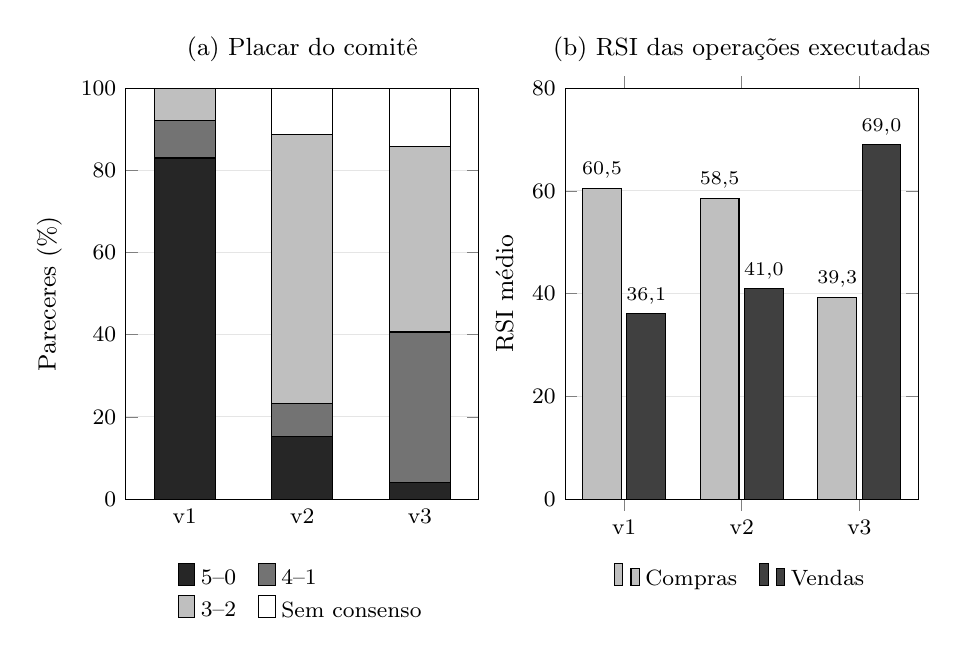
\begin{tikzpicture}
\begin{axis}[
  name=pa, ybar stacked, bar width=22pt, width=0.5\textwidth, height=6.8cm,
  symbolic x coords={v1,v2,v3}, xtick=data, ymin=0, ymax=100,
  enlarge x limits=0.25, ylabel={Pareceres (\%)}, title={(a) Placar do comitê},
  title style={font=\small}, label style={font=\small}, tick label style={font=\footnotesize},
  ymajorgrids, grid style={gray!20},
  legend style={at={(0.5,-0.14)}, anchor=north, legend columns=2, font=\footnotesize,
    draw=none, /tikz/every even column/.append style={column sep=6pt}},
  legend cell align=left,
]
\addplot[fill=black!85, draw=black] coordinates {(v1,83.01) (v2,15.13) (v3,4.03)};
\addlegendentry{5--0}
\addplot[fill=black!55, draw=black] coordinates {(v1,9.15) (v2,8.03) (v3,36.64)};
\addlegendentry{4--1}
\addplot[fill=black!25, draw=black] coordinates {(v1,7.84) (v2,65.66) (v3,45.10)};
\addlegendentry{3--2}
\addplot[fill=white, draw=black] coordinates {(v1,0) (v2,11.18) (v3,14.23)};
\addlegendentry{Sem consenso}
\end{axis}
\begin{axis}[
  at={(pa.east)}, anchor=west, xshift=1.1cm, ybar, bar width=14pt,
  width=0.5\textwidth, height=6.8cm,
  symbolic x coords={v1,v2,v3}, xtick=data, ymin=0, ymax=80,
  enlarge x limits=0.25, ylabel={RSI médio}, title={(b) RSI das operações executadas},
  title style={font=\small}, label style={font=\small}, tick label style={font=\footnotesize},
  ymajorgrids, grid style={gray!20}, nodes near coords,
  every node near coord/.append style={font=\scriptsize, /pgf/number format/fixed,
    /pgf/number format/precision=1, /pgf/number format/zerofill, /pgf/number format/use comma},
  legend style={at={(0.5,-0.14)}, anchor=north, legend columns=2, font=\footnotesize,
    draw=none, /tikz/every even column/.append style={column sep=6pt}},
  legend cell align=left,
]
\addplot[fill=black!25, draw=black] coordinates {(v1,60.51) (v2,58.54) (v3,39.26)};
\addlegendentry{Compras}
\addplot[fill=black!75, draw=black] coordinates {(v1,36.06) (v2,40.98) (v3,69.00)};
\addlegendentry{Vendas}
\end{axis}
\end{tikzpicture}
\caption{Comportamento do comitê e das operações da carteira Multiagentes por versão: (a) distribuição dos placares do sinal vencedor, em percentual dos pareceres com análise completa (765 na v1, 760 na v2 e 745 na v3); (b) RSI médio das compras e das vendas executadas.}
\label{fig:res-comite}
\par\smallskip\footnotesize Fonte: elaborado pelos autores, a partir do documento mestre do replay (\texttt{evolucao\_replay\_v1\_v2\_v3\_tcc.md}, Seção 5.4 e Tabela~\ref{tab:res-evolucao}); em cada versão, as quatro categorias do painel (a) somam 100\%.
\end{figure}

A Figura~\ref{fig:res-comite} mostra que a unanimidade da v1 deu lugar, na v2, a um comitê dominado por placares 3--2 e, na v3, a um comitê com predomínio de 3--2 e 4--1 e 14,23\% de pareceres sem consenso. O painel (b) mostra que a ordem dos RSI se inverteu apenas na v3: nas duas primeiras versões, as compras ocorreram com RSI mais alto que as vendas, e na v3, mais baixo.

\subsection{Diagnóstico da versão v1}
\label{sec:res-v1}

A auditoria da campanha v1 descartou a hipótese de ativo esquecido --- os cinco ativos foram analisados em todos os pregões, em 765 pareceres ativo-pregão --- e isolou cinco achados empíricos.

\begin{enumerate}
    \item \textbf{Trava de caixa.} O caixa livre ficou abaixo de R\$~200 em 69 dos 153 pregões, e o compilador estrito proibia reduzir uma posição cuja recomendação não fosse VENDA. A VALE3, zerada em 01/07, permaneceu fora da carteira por 94 pregões, até o fim da campanha, apesar de 14 recomendações de COMPRA aprovadas pelo risco entre 25/08 e 14/09, todas respondidas com HOLD; a ITUB4 recebeu 27 recomendações consecutivas de COMPRA (03/09 a 16/10) sem caixa para executá-las.
    \item \textbf{Compra no topo e venda no fundo.} O preço médio das compras superou o das vendas em quatro dos cinco ativos: WEGE3 (R\$~47,41 contra R\$~44,79), ITUB4 (R\$~44,07 contra R\$~40,61), VALE3 (R\$~83,46 contra R\$~78,85) e PETR4 (R\$~44,77 contra R\$~42,81). O sinal de COMPRA surgia com RSI médio de 63,17 e preço 7,82\% acima da média de 50 pregões; o de VENDA, com RSI médio de 35,07 e preço 8,64\% abaixo dela. Em WEGE3, único ativo em alta no período, o Buy \& Hold ganhou R\$~603,40 e a Bollinger 20/2, R\$~5.454,99, enquanto a v1 perdeu R\$~5.443,38 em três ciclos de saída e reentrada.
    \item \textbf{Veto de volatilidade bloqueando saídas.} Dos 41 vetos de risco, 40 decorreram da regra dura de volatilidade. Em 25 pares ativo-pregão havia consenso técnico de VENDA com posição aberta, concentrados em BBAS3 e ITUB4 entre 27/10 e 12/11, mas a conversão de VETADO em MANTER impediu a redução, justamente quando a volatilidade aumentava.
    \item \textbf{Concentração extrema e compras residuais.} Em 101 dos 153 pregões (66,01\%), a carteira teve apenas dois ativos com peso de pelo menos 2\%, com picos de 77,49\% em VALE3, 71,40\% em PETR4 e 66,05\% em WEGE3; no extremo oposto, houve oito compras com valor inferior a R\$~2.000.
    \item \textbf{Ausência de diversidade no comitê.} Das 765 votações, 635 (83,01\%) foram unânimes e nenhuma ficou sem consenso. Com o mesmo modelo, o mesmo \textit{prompt} e as mesmas evidências, a variação da semente, mesmo com temperatura 1,0, não produziu diversidade de critério: na prática, os cinco analistas atuaram como um único classificador de tendência.
\end{enumerate}

Os achados foram agrupados em quatro gargalos: trava de caixa (achado 1), concentração e ordens residuais (achado 4), veto simétrico (achado 3) e comitê homogêneo e pró-cíclico (achados 2 e 5). O quinto achado é coerente com a literatura discutida no Capítulo~\ref{cha:relacionados}, segundo a qual a agregação de respostas ajuda quando os raciocínios amostrados são diversos \citep{Wang2023} e seu benefício não é garantido, dependendo da configuração \citep{Smit2024}. A interpretação de que importa a diversidade efetiva entre os membros, e não apenas seu número, é deste trabalho.

\subsection{Versão v2: correções mecânicas e arrasto de caixa}
\label{sec:res-v2}

A v2 atacou os quatro gargalos com o \textit{Trim-to-Fund}, o teto de 30\% e a ordem mínima de R\$~2.000, o veto assimétrico (R7) e três lentes no comitê (Seção~\ref{sec:arq-evolucao}). O patrimônio final subiu R\$~3.564,86 (+3,56 pontos percentuais), para R\$~85.743,57, mas a carteira permaneceu em último lugar. Os efeitos sobre cada gargalo foram os seguintes:

\begin{itemize}
    \item \textbf{Trava de caixa:} duas reduções \textit{Trim-to-Fund} em PETR4 (15/09 e 15/10) e reentrada de VALE3 em 01/09;
    \item \textbf{Concentração:} nenhuma compra abaixo de R\$~2.000, 99 pregões com três ou mais ativos relevantes e 26 ajustes do compilador (15 de teto e 11 de ordem mínima);
    \item \textbf{Veto:} 12 casos de VENDA sob veto e duas saídas executadas sob R7 (ITUB4 em 27/10 e BBAS3 em 09/11), que evitaram cerca de R\$~827,34 de perda adicional até 12/11;
    \item \textbf{Comitê:} a unanimidade caiu de 83,01\% para 15,13\%, com 499 placares de consenso mínimo (65,66\%) e 85 pareceres sem consenso.
\end{itemize}

A melhora concentrou-se em um único ativo: o ganho de R\$~3.596,27 em PETR4 supera o ganho total da versão, e os outros quatro ativos, somados, pioraram R\$~31,41. Três limitações persistiram. Primeiro, a quebra da unanimidade não alterou o momento das decisões na mesma proporção: o perfil de execução continuou pró-cíclico, com RSI médio de 58,54 nas compras e 40,98 nas vendas. O diagnóstico atribui esse viés ao desempate pelo analista de regime nos placares 3--2, interpretação que os dados confirmam quanto à contagem dos placares e ao perfil resultante, mas não quanto ao voto de cada cadeira. Segundo, dez das 16 vendas zeraram a posição, e o preço médio de compra superou o de venda em quatro ativos (WEGE3, VALE3, ITUB4 e BBAS3); PETR4 foi o único ativo sem saída total e o único com resultado positivo.

Terceiro, surgiu um arrasto de caixa (\textit{cash drag}). As recomendações de COMPRA caíram de 273 na v1 para 106 na v2, contra 537 de MANTER, e o teto de 30\% por ativo limitou a reaplicação do caixa: o caixa médio foi de 24,69\% do patrimônio, superou 30\% em 65 pregões, atingiu 67,74\% e terminou em 45,86\%, com a carteira posicionada em apenas dois ativos (455 PETR4 e 490 WEGE3) e R\$~39.321,44 em caixa não remunerado. Com dois ativos e teto de 30\% cada, ao menos 40\% do capital fica estruturalmente parado. A Figura~\ref{fig:replay-caixa} mostra a trajetória do caixa nas três versões.

% Gerado por tcc2/scripts/metricas_replay.py; requer \usepackage{pgfplots}.
\begin{figure}[htbp]
\centering
\begin{tikzpicture}
\begin{axis}[
  width=\textwidth, height=7.5cm, xmin=0, xmax=153,
  xtick={0,19,39,60,83,104,125,146},
  xticklabels={abr,mai,jun,jul,ago,set,out,nov},
  xlabel={Pregão (2026)}, ylabel={Caixa (\% do patrimônio)},
  ymajorgrids, grid style={gray!20}, tick label style={font=\footnotesize},
  label style={font=\small}, scaled y ticks=false,
  yticklabel style={/pgf/number format/use comma, /pgf/number format/1000 sep={.}},
  legend style={at={(0.5,-0.2)}, anchor=north, legend columns=3,
    font=\footnotesize, draw=none, /tikz/every even column/.append style={column sep=6pt}},
  legend cell align=left, ymin=0,
]
\addplot[black, thick, densely dotted] table[x=idx, y=cx_ma_v1, col sep=comma] {figures/replay-series.csv};
\addlegendentry{Multiagentes v1}
\addplot[black, thick, dashed] table[x=idx, y=cx_ma_v2, col sep=comma] {figures/replay-series.csv};
\addlegendentry{Multiagentes v2}
\addplot[black, very thick] table[x=idx, y=cx_ma_v3, col sep=comma] {figures/replay-series.csv};
\addlegendentry{Multiagentes v3}
\end{axis}
\end{tikzpicture}
\caption{Caixa em percentual do patrimônio das três versões da carteira Multiagentes no Replay Contínuo.}
\label{fig:replay-caixa}
\end{figure}


\subsection{Versão v3: especialização do comitê e governança do gestor}
\label{sec:res-v3}

A v3 manteve a topologia 5 + 1 + 1 e alterou a composição do comitê e as regras do gestor: cinco lentes especialistas distintas, travas sobre consensos mínimos em extremos, memória contábil de posição, piso de posição-núcleo de 8\%, venda escalonada limitada a 45\% da posição, regra contra recompra mais cara e recomposição contra o arrasto de caixa (Seção~\ref{sec:arq-evolucao}). O patrimônio final foi de R\$~100.067,36 (+0,07\%), R\$~14.323,79 acima da v2 e R\$~17.888,65 acima da v1. A carteira ficou acima do Buy \& Hold (+R\$~11.276,25), da SMA 50/200 (+R\$~11.200,68), da Equal Weight 63d (+R\$~10.198,07) e da Mínima Variância 252/63 (+R\$~4.252,52), e abaixo da Bollinger 20/2 ($-$R\$~4.819,69). Os efeitos observados foram os seguintes.

\paragraph*{Diversidade do comitê.} A unanimidade caiu para 4,03\% dos pareceres, com 36,64\% de placares 4--1, 45,10\% de 3--2 e 14,23\% sem consenso.

\paragraph*{Inversão do perfil de execução.} A relação entre sinal e estado técnico do ativo, pró-cíclica nas duas primeiras versões, inverteu-se. O RSI médio do sinal de COMPRA passou a 35,11 e o do sinal de VENDA, a 68,96; nas operações executadas, a 39,26 nas compras e 69,00 nas vendas. A diferença entre o RSI médio das compras e o das vendas executadas passou de +24,45 (v1) e +17,56 (v2) para $-29{,}74$. As compras ocorreram, em média, com preço 3,69\% abaixo da média de 50 pregões e a 0,93\% da banda inferior; as vendas, com preço 11,09\% acima dessa média e a 0,52\% da banda superior.

\paragraph*{Saídas totais e preço médio.} A v3 não zerou nenhuma posição, contra nove saídas na v1 e dez na v2, e manteve os cinco ativos com peso de pelo menos 2\% em todos os 153 pregões. O preço médio de venda superou o de compra nos cinco ativos: PETR4 (R\$~43,18 para R\$~46,43), WEGE3 (R\$~48,13 para R\$~48,61), ITUB4 (R\$~42,14 para R\$~44,47), BBAS3 (R\$~20,37 para R\$~21,48) e VALE3 (R\$~75,77 para R\$~81,13).

\paragraph*{Proventos e caixa.} Por nunca zerar posições antes das datas-com, a carteira recebeu os 20 eventos de proventos do período (R\$~1.425,30 líquidos), contra nove eventos na v1 (R\$~567,02) e nove na v2 (R\$~509,28). O caixa médio caiu de 24,69\% para 14,94\% do patrimônio e o caixa final, de 45,86\% para 0,75\% (Figura~\ref{fig:replay-caixa}).

\paragraph*{Resultado por ativo.} WEGE3 (+R\$~1.991,89) e ITUB4 (+R\$~1.435,82) passaram a resultado positivo, e PETR4 permaneceu positivo (+R\$~3.222,19); WEGE3 e ITUB4 respondem por R\$~12.089,35 (84,4\%) do ganho sobre a v2. BBAS3 ($-$R\$~1.997,86) e VALE3 ($-$R\$~4.584,68), os dois ativos que mais caíram, permaneceram negativos. Em VALE3, a v3 teve o pior resultado das três versões e ficou abaixo do Buy \& Hold ($-$R\$~4.255,30): o piso de posição-núcleo, que evita saídas totais, também impõe exposição a ativos em queda persistente.

\paragraph*{Mecanismos efetivamente acionados.} Dos 80 ajustes registrados pelo compilador, 56 foram de piso núcleo e venda escalonada (\texttt{CORE\_FLOOR\_STEP\_SELL}), 12 de teto de peso, 9 de ordem mínima, 2 de caixa insuficiente e 1 de teto da recomposição; houve duas compras de recomposição. Não foram acionados, no período, as travas de extremo do comitê, o \textit{Trim-on-Strength}, o \textit{Trim-to-Fund}, o corte por recompra mais cara nem a saída sob R7. As 52 vendas ocorreram todas sob consenso técnico de VENDA com risco aprovado, dosadas pelo piso núcleo. O efeito observado deve-se, portanto, à combinação de lentes, piso núcleo, venda escalonada, teto, ordem mínima e recomposição, e não aos mecanismos que permaneceram inativos. Os 80 ajustes indicam ainda que a proposta bruta do gestor violava as regras com frequência, sobretudo ao pedir vendas maiores que as permitidas: a governança determinística também moldou o resultado: 80 ajustes, 56 deles limitando vendas, alteraram a proposta bruta do gestor. O desenho, sem ablação, não permite medir quanto do resultado se deve a ela e quanto aos sinais.

\paragraph*{Efeitos colaterais.} Das 52 vendas, 27 tiveram valor inferior a R\$~2.000 (22 abaixo de R\$~500), somando R\$~7.970,68: são vendas residuais produzidas pelo piso núcleo, que, com a posição próxima de 8\% do patrimônio, libera apenas as poucas ações excedentes a cada novo sinal de VENDA. Esse padrão é favorecido pelo custo puramente proporcional do replay e seria inviável com custo fixo ou lote mínimo. Os quatro pregões sem análise da v3 ocorreram após chamadas bem-sucedidas, na validação da resposta do gestor: em três deles (01/07, 01/09 e 02/10), o gestor expressou ``não vender'' como venda de quantidade zero para ativos junto ao piso, e no quarto (01/10) a resposta não cobria o universo completo.

\section{Discussão}
\label{sec:res-discussao}

\paragraph*{O que os resultados permitem afirmar.} Primeiro, no replay, H1 e H2 não são sustentadas: H0 não é rejeitada para o contraste de tendência contra pesos iguais nem para a família de contrastes da carteira Multiagentes pré-especificada. Segundo, a versão pré-especificada teve, descritivamente, o menor patrimônio final, o maior \textit{drawdown} máximo e o maior giro entre as oito carteiras, e a auditoria identificou os mecanismos que produziram esse resultado; trata-se de um resultado negativo, registrado como tal. Terceiro, dentro desta trajetória e sob estas regras, a especialização das lentes e a governança determinística mudaram de forma mensurável o comportamento da carteira: menos unanimidade, inversão do momento de compra e venda, fim das saídas totais, menor concentração, captura integral de proventos e patrimônio final R\$~17.888,65 acima da linha de base. Quarto, mantido o número de agentes, a diversidade efetiva do comitê dependeu da diferenciação das funções atribuídas a eles: sementes distintas não produziram diversidade, e lentes duplicadas formaram blocos de voto que reproduziram o viés do bloco majoritário.

\paragraph*{O que os resultados não permitem afirmar.} Os resultados não permitem afirmar que a v3 seja superior às referências fora deste período, que a ordenação se repita em outro regime, que algum mecanismo isolado seja responsável pelo ganho ou que o resultado represente benefício financeiro esperado. As razões são as ameaças da Seção~\ref{sec:met-ameacas}, que se manifestam concretamente nos resultados:

\begin{itemize}
    \item \textbf{Ajuste dentro da amostra.} A v2 e a v3 foram desenhadas após a observação das campanhas anteriores nos mesmos 153 pregões, com limiares escolhidos com conhecimento do período, e a v3 foi desenhada quando já se sabia que a Bollinger 20/2 era a referência de melhor resultado. Não há amostra de validação. A melhora de 17,89 pontos percentuais da v1 para a v3 mede a capacidade da arquitetura de incorporar correções dentro da amostra, e não desempenho esperado fora dela \citep{White2000, Bailey2017}.
    \item \textbf{Intervenções em bloco.} Cada versão alterou vários fatores simultaneamente, sem ablação, e parte dos mecanismos da v3 não foi acionada. A contribuição de cada pilar não é identificável.
    \item \textbf{Possível contaminação.} As campanhas foram executadas em 13, 15 e 16/11/2026, depois do período, com um modelo cujo corte de conhecimento declarado não é verificável e cujo identificador não garante versão imutável. A contaminação, se existir, tende a favorecer a carteira Multiagentes \citep{ProfitMirage2025, Wang2026}, embora o conhecimento prévio também possa prejudicar \citep{Glasserman2023}: ela não explica o desempenho inferior da v1, mas pode ter contribuído para o da v3. O gestor, único papel que recebe \textit{tickers}, datas e preços, é o canal exposto; as referências determinísticas e o contraste de H1 não são afetados.
    \item \textbf{Uma execução por versão.} Com temperatura 1,0, cada campanha é uma realização de um processo estocástico; sem repetições, a variância entre execuções não é estimada, e as diferenças entre versões incluem esse componente aleatório, além das diferenças no número de pregões sem análise (0, 1 e 4) e na data de execução sob o mesmo \textit{alias} do modelo.
    \item \textbf{A melhor referência é uma regra simples.} A Bollinger 20/2, determinística e sem custo de inferência, terminou R\$~4.819,69 acima da v3, com Sharpe maior (0,73 contra 0,09) e \textit{drawdown} máximo menor ($-8{,}52\%$ contra $-12{,}80\%$). As lentes da v3 codificam, em boa medida, a lógica de reversão à média que caracteriza essa referência. A leitura cautelosa é que a arquitetura multiagente se mostrou capaz de expressar uma política de reversão à média com governança de carteira, e não que tenha descoberto uma política superior.
    \item \textbf{Dependência de regime.} Quatro dos cinco ativos caíram e a referência de tendência ficou próxima do Buy \& Hold. Em um período de tendência persistente, vender força e comprar fraqueza poderia inverter a ordenação das versões e das referências; o replay não permite avaliar essa possibilidade.
    \item \textbf{Custo de inferência.} Cada campanha realizou cerca de 4.703 chamadas lógicas ao modelo, com custo conhecido estimado de US\$~7,44 (v1), US\$~8,92 (v2) e US\$~8,63 (v3), não deduzido do patrimônio. As referências não têm esse custo. A v3 consumiu, assim, cerca de US\$~8,63 em inferência para terminar abaixo de uma regra determinística.
    \item \textbf{Exposição ao mercado e caixa.} Em um período de queda, a exposição média explica parte da ordenação: a Bollinger 20/2 manteve, em média, cerca de metade do patrimônio em caixa (49,06\%), o que atenua a perda por si só. A v3, majoritariamente investida (caixa médio de 14,94\%), terminou 11,28 pontos percentuais acima do Buy \& Hold, diferença associada ao perfil de execução e aos proventos (Seção~\ref{sec:res-v3}). O caixa não rende juros e a taxa livre de risco é nula ($r_f = 0$), o que penaliza as carteiras com mais caixa. O trabalho não decompõe os retornos em fatores, porque 153 pregões e cinco ações são poucos para estimar exposições com confiança; a parte da ordenação atribuível à exposição é apenas indicada pelo caixa médio. Em avaliações de agentes LLM de negociação com essa decomposição, a exposição a mercado e estilo explicou a maior parte do retorno \citep{Wang2026beta}. No período, o CDI acumulou 8,33\% \citep{BCBCDI2026}, valor que nenhuma carteira superou (a maior, a Bollinger 20/2, rendeu +4,89\%): medido contra o CDI, nenhum resultado foi positivo.
    \item \textbf{Propriedades das métricas.} Com retornos médios negativos, o Sharpe penaliza as carteiras menos voláteis, o que afeta os contrastes que envolvem a SMA 50/200; com taxa livre de risco nula, todos os índices ficam acima do que seriam sob uma taxa de juros positiva. A execução simplificada, sem custo fixo, \textit{spread} ou impacto, favorece estratégias com muitas operações pequenas, como a v3.
\end{itemize}

Em síntese, o replay oferece evidência descritiva sobre como mudanças de arquitetura alteram o comportamento de uma carteira multiagente em uma trajetória conhecida, mas não oferece evidência de superioridade dos agentes sobre as referências. O passo que poderia converter os achados exploratórios em evidência fora da amostra é a avaliação prospectiva de uma versão congelada da carteira, sem novos ajustes, no regime descrito na Seção~\ref{sec:met-protocolo}.

\section{Acompanhamento Prospectivo Preliminar}
\label{sec:obs-operacional}

Independentemente do replay, o acompanhamento diário prospectivo da carteira multiativos (Seção~\ref{sec:met-protocolo}) teve início em 14/10/2026, com as carteiras Multiagentes e Buy \& Hold montadas com a mesma cesta inicial (\mbox{DP-20}) e capital de R\$~100.000,00 cada, em regime de simulação, sem capital real nem envio de ordens. O ciclo diário autônomo (\mbox{DP-34}), descrito na Seção~\ref{sec:arq-operacao-diaria}, foi adotado a partir de 20/10/2026. O acompanhamento opera a arquitetura da v1: o ciclo diário usa os módulos originais da carteira, e as regras da v2 e da v3 existem apenas nos \textit{scripts} do replay. Esse acompanhamento não integra os resultados anteriores: suas carteiras, sua cesta e sua data de início são distintas das do replay, e suas decisões são registradas antes de o desfecho existir.

A série diária das quatro carteiras do acompanhamento foi exportada do servidor de operação em 17/11/2026 (\texttt{tcc2/evidence/06-operacao-diaria/serie-diaria-20261117/}) e cobre 23 pregões fechados, de 14/10 a 16/11/2026. Além de Multiagentes e Buy \& Hold, a série inclui as carteiras SMA 50/200 e Bollinger 20/2 (\mbox{DP-36}), criadas sobre a mesma cesta de 14/10. Nenhuma das duas regras emitiu sinal no período, e suas curvas coincidem com a do Buy \& Hold. O Buy \& Hold não negociou após a montagem da cesta; sua trajetória, de R\$~99.835,33 no fechamento de 14/10 para R\$~82.391,17 em 16/11, perda de $17{,}61\%$ sobre o capital inicial de R\$~100.000,00, reflete apenas a variação de preços dos cinco ativos. A Multiagentes realizou 19 operações após a entrada e terminou em R\$~76.059,11 ($-23{,}94\%$ sobre o capital inicial). Ela esteve à frente do Buy \& Hold até 23/10, com vantagem máxima de R\$~2.265,83 nessa data, mas caiu mais na queda de 26/10 (R\$~84.601,02 contra R\$~86.869,15) e ampliou a desvantagem nas semanas seguintes, até R\$~6.332,06 em 16/11. Nas duas carteiras, o \textit{drawdown} máximo do período coincide com a perda acumulada, tomando-se o capital inicial como pico, pois o último fechamento é também o vale.

Essas observações cobrem poucas semanas e uma queda concentrada de mercado, e não sustentam métricas de risco nem inferência sobre as hipóteses. Seu papel no trabalho é registrar o início do regime de avaliação compatível com a \mbox{DP-31}, no qual a contaminação do modelo pelo resultado é excluída por construção.

\chapter{Conclusão}
\label{cha:conclusao}

% Fontes: Capítulos 4 e 5; tcc2/agent-reports/METRICAS_REPLAY.md; tcc2/agent-reports/BOOTSTRAP_REPLAY.md;
% tcc2/evidence/04-replay-abril-novembro/relatorios/evolucao_replay_v1_v2_v3_tcc.md (seções 4.7, 5.9, 5.10 e 6).
Este capítulo sintetiza o que foi construído, responde à pergunta de pesquisa, às hipóteses H1, H2 e H0 e à pergunta arquitetural formuladas no Capítulo~\ref{cha:introducao}, e registra as limitações do estudo e os trabalhos futuros que delas decorrem.

\section{Síntese do Trabalho}

O trabalho desenvolveu o Hedge-fund-lab, um laboratório quantitativo para a avaliação de estratégias de investimento baseadas em sistemas multiagentes. O laboratório compreende um pipeline de dados construído sobre o arquivo oficial de cotações da B3 (COTAHIST), com fator de ajuste por proventos, calendário de negociação próprio e persistência relacional; um motor de \textit{backtesting} com a definição congelada do Sharpe Ratio líquido; um livro contábil de eventos imutáveis, encadeados por \textit{hash}, no qual posições e caixa são recalculados a cada leitura; e dois caminhos de decisão multiagente --- o grafo LangGraph de ativo único e a carteira multiativos, composta por comitês de analistas técnicos por ativo, analista de risco por ativo, gestor global da carteira e compilador determinístico da proposta do modelo (Capítulo~\ref{cha:arquitetura}).

Sobre essa base foram construídos o Replay Contínuo Abril--Novembro de 2026, com relógio causal por pregão, orçamento de inferência com reserva anterior a cada requisição, tratamento \textit{fail-closed} de pregões sem decisão válida, pacotes selados e auditorias de paridade das carteiras de referência; e o ciclo diário autônomo que opera a carteira multiativos de forma prospectiva desde 14/10/2026, com a arquitetura da v1. O desenho experimental do replay é pareado: as seis carteiras partem da mesma cesta, nas mesmas sessões, com os mesmos preços e custos, e as hipóteses são decididas pelo Sharpe líquido com o Bootstrap A (Capítulo~\ref{cha:metodologia}).

Em nenhuma etapa o modelo de linguagem foi treinado. O \texttt{gemini-3.8-flash} foi utilizado pré-treinado, sem ajuste fino; o que se calibrou --- no protocolo planejado de ativo único e, de modo exploratório, nas versões v2 e v3 do replay --- foi a configuração do sistema: \textit{prompts}, composição do comitê, regras de agregação e de veto, contexto do gestor e regras determinísticas do compilador. Calibração, neste trabalho, designa o ajuste dessa configuração, e não o treinamento do modelo.

Os seis objetivos específicos do Capítulo~\ref{cha:introducao} foram atendidos. O \textit{pipeline} de dados sobre o COTAHIST, com correção de proventos e calendário próprio, e o motor de \textit{backtesting} com o livro contábil de eventos (objetivos 1 e 2) estão descritos no Capítulo~\ref{cha:arquitetura}. Os dois caminhos multiagentes, de ativo único e multiativos (objetivo 3), também estão nesse capítulo. O desenho pareado, com a métrica primária e a regra de decisão estatística (objetivo 4), está no Capítulo~\ref{cha:metodologia}. O Replay Contínuo nas três versões, com decisões, operações e patrimônio rastreáveis (objetivo 5), foi executado e analisado no Capítulo~\ref{cha:resultados}. O acompanhamento diário prospectivo (objetivo 6) está em curso desde 14/10/2026, com a arquitetura da v1 (Seção~\ref{sec:obs-operacional}); sua avaliação, por depender de um horizonte maior, permanece como trabalho futuro.

\section{Resposta à Pergunta de Pesquisa e às Hipóteses}

A pergunta de pesquisa tem duas partes. Quanto ao ambiente experimental, o trabalho apresenta uma forma de realizá-lo: carteiras pareadas com estado inicial comum, separação entre os dados entregues à decisão e os preços de execução e marcação, referências determinísticas reproduzidas com paridade exata entre campanhas, métrica primária e regra de decisão herdadas do protocolo anterior ao \textit{replay} (o mapeamento das hipóteses nos contrastes --- H1 em SMA 50/200 contra Equal Weight 63d e a família de cinco contrastes de H2 com ajuste de Holm --- foi definido na redação, depois do replay, sem seleção entre alternativas; Seção~\ref{sec:met-hipoteses}) e registro auditável de cada voto, parecer, intervenção do compilador, operação e patrimônio diário. Esse ambiente permitiu identificar, por auditoria, os gargalos que explicam o desempenho da versão inicial e comparar versões sucessivas da arquitetura sob condições constantes. Quanto à robustez das decisões, a resposta obtida nesta trajetória é que não há evidência de que a arquitetura multiagente produza decisões superiores às das abordagens tradicionais.

\paragraph*{H1.} A SMA 50/200 obteve Sharpe líquido de $-1{,}42$, contra $-0{,}71$ da Equal Weight 63d ($\hat{\Delta} = -0{,}71$; $p_{+} = 0{,}881$; intervalo bilateral de 90\% $[-1{,}75;\ 0{,}31]$). H0 não é rejeitada: o contraste tem o sinal oposto ao previsto por H1, e o intervalo, que contém zero, também não indica inferioridade. Por envolver apenas carteiras determinísticas, esse resultado não é afetado pela possível contaminação do modelo, mas seu alcance restringe-se a uma única regra de tendência com uma parametrização, e não à família de estratégias de \textit{momentum} e \textit{trend following}.

\paragraph*{H2.} A versão pré-especificada (v1), a única a receber decisão inferencial, condicionada à possível contaminação do modelo, terminou com patrimônio de R\$~82.178,71 ($-17{,}82\%$), abaixo das cinco referências, e Sharpe líquido de $-1{,}28$, inferior ao de quatro delas --- Buy \& Hold ($-0{,}78$), Bollinger 20/2 ($0{,}73$), Equal Weight 63d ($-0{,}71$) e Mínima Variância 252/63 ($-0{,}32$) --- e superior apenas ao da SMA 50/200 ($\hat{\Delta} = 0{,}14$; $p_{+} = 0{,}432$). Nenhuma das cinco comparações atende à regra de superioridade, com ou sem a correção de Holm, e o enunciado de superioridade em relação ao conjunto dos \textit{benchmarks} não é sustentado. Os critérios complementares apontam na mesma direção: a v1 teve o maior \textit{drawdown} máximo entre as oito carteiras ($-22{,}90\%$) e o maior giro (6,78 vezes o patrimônio médio).

\paragraph*{H0.} H0 não é rejeitada em nenhuma das duas famílias. A não rejeição, contudo, não demonstra igualdade de desempenho. Com 153 pregões, o erro-padrão aproximado do Sharpe anualizado é de ao menos cerca de 1,3 sob retornos independentes \citep{Lo2002}, e os intervalos de 90\% dos contrastes têm amplitude entre 2,1 e 4,9 pontos de Sharpe; diferenças economicamente relevantes, em qualquer direção, não se distinguem do ruído amostral nesta janela.

\paragraph*{Versões exploratórias.} A v2 e a v3 são iterações exploratórias, ajustadas dentro da amostra, e recebem apenas descrição. A v2 terminou em R\$~85.743,57 ($-14{,}26\%$) e não atingiu a regra de superioridade em nenhuma comparação. A v3 terminou em R\$~100.067,36 ($+0{,}07\%$), com Sharpe de $0{,}09$, acima de quatro referências e abaixo da Bollinger 20/2 (R\$~104.887,05; $+4{,}89\%$). O único contraste com valor-$p$ bruto inferior a 0,05 --- v3 contra a SMA 50/200, referência de pior Sharpe no período ($\hat{\Delta} = 1{,}50$; $p_{+} = 0{,}024$) --- é descritivo: não resiste ao ajuste de Holm na família da v3 ($p_{+}$ ajustado de 0,121) e, sobretudo, provém de uma versão cujas regras foram escolhidas com conhecimento do mesmo período, o que retira desse valor-$p$ a interpretação de teste \citep{White2000, Bailey2017}. Os resultados de v2 e v3 são descritivos: não rejeitam H0 e não constituem evidência de superioridade.

\section{Resposta à Pergunta Arquitetural}

Mantidos o modelo, a topologia de agentes, os dados, a execução e as referências, a diferença de patrimônio final entre a v1 e a v3 foi de R\$~17.888,65 (17,89 pontos percentuais). Nesta trajetória, portanto, o comportamento da carteira multiagente dependeu fortemente da composição do comitê e das regras determinísticas aplicadas à proposta do gestor, como indicam a queda da unanimidade (83,01\% para 4,03\%) e a inversão do perfil de execução; a diferença de patrimônio inclui, além das intervenções, a variabilidade de uma única execução por versão. Quatro observações descritivas detalham e qualificam essa leitura.

Primeiro, a diversidade do comitê exigiu especialização. Na v1, cinco instâncias do mesmo modelo, com o mesmo \textit{prompt} e sementes diferentes, foram unânimes em 83,01\% dos pareceres, mesmo com temperatura 1,0; a variação estocástica não produziu diversidade de critério. Com três lentes analíticas (v2), a unanimidade caiu para 15,13\% e, com cinco lentes distintas (v3), para 4,03\%.

Segundo, quebrar a unanimidade não bastou. Na v2, com lentes duplicadas formando blocos de voto, o perfil de execução permaneceu pró-cíclico (RSI médio de 58,54 nas compras e 40,98 nas vendas). Apenas na v3 o perfil se inverteu (39,26 nas compras e 69,00 nas vendas), com preço médio de venda superior ao de compra nos cinco ativos, nenhuma posição zerada e recebimento dos 20 eventos de proventos do período.

Terceiro, a governança determinística também moldou o resultado. O modelo propõe e o compilador limita, ajusta e registra: a melhora da v1 para a v2 foi associada, na auditoria, principalmente às regras de carteira impostas sobre a proposta, e na v3 o compilador realizou 80 ajustes, dos quais 56 limitaram vendas ao piso de posição-núcleo e à venda escalonada. O desenho, sem ablação, não permite medir quanto do resultado se deve a essa governança e quanto aos sinais. A separação entre o julgamento do modelo e a execução das regras é, nesse sentido, um componente da arquitetura, e não um detalhe de implementação.

Quarto, uma regra simples permaneceu à frente. A Bollinger 20/2, determinística e sem custo de inferência, terminou R\$~4.819,69 acima da v3. As lentes da v3 codificam, em boa medida, a lógica de reversão à média dessa referência, que já era conhecida como a de melhor resultado quando a v3 foi desenhada. A leitura cautelosa é que a arquitetura se mostrou capaz de expressar uma política de reversão à média com governança de carteira, e não que tenha descoberto uma política superior; em um regime de tendência persistente, vender força e comprar fraqueza poderia inverter a ordenação das versões.

Essas observações valem para esta trajetória e para o conjunto de intervenções de cada versão. Elas não identificam o efeito de cada mecanismo isoladamente: parte dos mecanismos da v3 não foi acionada no período (as travas sobre consensos em extremos, as vendas parciais fora de recomendação de venda e a saída sob veto), as versões diferem no número de pregões sem análise (nenhum na v1, um na v2 e quatro na v3) e não há garantia de que o modelo servido sob o mesmo identificador tenha sido idêntico nas três datas de execução.

\section{Limitações}

As principais limitações, discutidas na Seção~\ref{sec:met-ameacas}, são:

\begin{itemize}
    \item \textbf{Contaminação do modelo pelo período.} O replay foi produzido depois do fim do período, e o corte de conhecimento declarado do modelo (março de 2026) não é verificável. A contaminação, se existir, tende a favorecer a carteira Multiagentes \citep{ProfitMirage2025, Wang2026}; por isso, mesmo um resultado favorável do replay não seria evidência prospectiva. O gestor, único papel que recebe \textit{tickers}, datas e preços, é o canal exposto; as referências determinísticas e o contraste de H1 não são afetados.
    \item \textbf{Ajuste dentro da amostra.} As versões v2 e v3 foram desenhadas após a observação das anteriores nos mesmos 153 pregões, sem amostra de validação; seus resultados são otimistas por construção e podem refletir sobreajuste a esta trajetória.
    \item \textbf{Amostra única e baixo poder.} Uma única trajetória de 153 pregões, um único regime de mercado e uma única execução por versão, com modelo estocástico, sem estimativa da variância entre execuções.
    \item \textbf{Escopo reduzido.} Cinco ações do mercado brasileiro, cesta inicial imposta e comum a todas as carteiras, e H1 respondida por uma única regra de tendência.
    \item \textbf{Execução simplificada.} Abertura oficial diária como aproximação do leilão, sem \textit{spread}, impacto de mercado ou liquidação em D+2; custo proporcional sem custo fixo nem lote mínimo; custo de inferência (US\$~8,63 na v3) não deduzido do patrimônio.
    \item \textbf{Seleção do universo.} Os cinco ativos foram fixados antes do replay, mas já eram conhecidos; a escolha afeta mais os níveis de desempenho do que as comparações pareadas.
    \item \textbf{Caixa, taxa livre de risco e tributação.} O caixa não rende juros e $r_f = 0$, o que penaliza as carteiras com mais caixa; no período, o CDI acumulou 8,33\% \citep{BCBCDI2026}, e nenhuma carteira o superou. Não há imposto sobre ganho de capital, embora o JCP seja tributado.
    \item \textbf{Múltiplas comparações e fatores de ajuste.} Os 16 contrastes e as iterações v2 e v3 ampliam a chance de achados espúrios; os fatores de ajuste por proventos foram adquiridos depois do período, e a ausência de vazamento para as \textit{features} não foi demonstrada.
    \item \textbf{Acompanhamento prospectivo.} Até aqui, só a arquitetura da v1 opera no acompanhamento, e a janela é curta.
    \item \textbf{Intervenções em bloco e sem decomposição em fatores.} Cada versão alterou vários fatores simultaneamente, sem ablação, o que impede atribuir efeito a mecanismos isolados; os retornos tampouco foram decompostos em fatores, de modo que exposição ao mercado e habilidade não são separadas.
    \item \textbf{Protocolo confirmatório não executado.} O desenho original, com calibração e avaliação separadas temporalmente, três execuções do modelo e um Teste Final isolado, não foi concluído; o replay herdou dele a métrica e o procedimento inferencial, mas não a separação temporal nem as repetições.
\end{itemize}

\section{Trabalhos Futuros}

As limitações indicam os próximos passos:

\begin{itemize}
    \item \textbf{Avaliação prospectiva com regras congeladas.} Congelar as regras da v3, sem novos ajustes de parâmetro, e avaliá-las no acompanhamento diário prospectivo, com hipótese, métrica e regra de decisão registradas antes da coleta. É o passo que poderia converter os achados exploratórios do replay em evidência fora da amostra.
    \item \textbf{Múltiplas execuções do modelo.} Repetir as campanhas, como previa o protocolo original, para estimar a variância entre execuções e incorporá-la à inferência.
    \item \textbf{Decomposição em fatores.} Decompor os retornos das carteiras em mercado, estilo e alfa, para separar exposição de habilidade \citep{FamaFrench1993, Wang2026beta}, com uma janela e um universo suficientes para estimar as exposições.
    \item \textbf{Universo e períodos ampliados.} Avaliar mais ativos, outros mercados e outros regimes, inclusive de tendência persistente, e outras parametrizações das regras de \textit{momentum}.
    \item \textbf{Ablação dos pilares.} Isolar a contribuição de cada mecanismo da v3 (lentes especialistas, piso de posição-núcleo e venda escalonada, vendas parciais e recomposição de caixa) sobre a v2.
    \item \textbf{Controle da contaminação.} Empregar modelos com corte de conhecimento verificável e versões imutáveis, anonimizar os ativos apresentados ao gestor e aplicar testes de detecção de contaminação.
    \item \textbf{Refinamentos de execução e contabilidade.} Normalizar ações de quantidade zero para manutenção antes da validação da proposta, remunerar o caixa por uma taxa de referência, introduzir custos fixos e lotes mínimos e deduzir o custo de inferência do resultado da carteira.
\end{itemize}

\section{Considerações Finais}

O Hedge-fund-lab cumpriu o papel de laboratório: permitiu comparar, sob condições controladas e auditáveis, uma carteira decidida por agentes baseados em LLMs com carteiras de referência clássicas e examinar como a especialização dos agentes e a governança determinística alteram o comportamento da carteira. Na execução pré-especificada, a carteira multiagente não superou as referências; na iteração exploratória v3, ajustada dentro da amostra e apenas descrita, terminou acima de quatro referências e abaixo da regra determinística de melhor resultado, em resultado otimista por construção. O replay é retrospectivo; a avaliação da v3 com regras congeladas é trabalho futuro. Os resultados não autorizam nenhuma expectativa de desempenho futuro: o benefício financeiro de agentes baseados em LLMs permanece uma hipótese a investigar, cuja avaliação compatível com as limitações aqui registradas é o acompanhamento prospectivo, com regras congeladas antes de o desfecho existir.


\backmatter

\referencepage % Comando do molde para renderizar o arquivo "references.bib"

\appendix
% Apêndices (pós-textuais, depois das referências). Cada \chapter vira
% "APÊNDICE X – TÍTULO" em página própria; o conteúdo começa na página seguinte.

\chapter{Mapa de Implementação}
\label{ap:mapa}

Este apêndice relaciona os componentes descritos no Capítulo~\ref{cha:arquitetura} aos arquivos do repositório e reúne os detalhes de implementação que não sustentam a argumentação do corpo do texto.

\section{Tecnologias da implementação}

A Tabela~\ref{tab:stack} lista as tecnologias empregadas. O sistema usa Python como linguagem base e não depende de framework web: o servidor HTTP é da biblioteca padrão, com tratamento concorrente de requisições (\texttt{socketserver.ThreadingMixIn}). A simulação histórica clássica é executada por um motor de \textit{backtesting} próprio, independente de bibliotecas externas.

\begin{table}[htbp]
\centering
\caption{Tecnologias da implementação do Hedge-fund-lab.}
\label{tab:stack}
\small
\begin{tabular}{>{\raggedright\arraybackslash}p{3.8cm} >{\raggedright\arraybackslash}p{11.2cm}}
\toprule
\textbf{Camada} & \textbf{Tecnologia utilizada} \\
\midrule
Servidor HTTP & \texttt{http.server}/\texttt{socketserver} (biblioteca padrão), \texttt{dashboard/server.py} \\
Frontend & HTML/CSS/JS + Chart.js (\texttt{dashboard/}) \\
Persistência de séries & SQLAlchemy, URL configurável, padrão SQLite (\texttt{src/db}) \\
Livro das carteiras & SQLite direto, eventos encadeados (\texttt{dashboard/manual\_portfolio\_api.py}) \\
Orquestração (ativo único) & LangGraph (\texttt{src/agents}) \\
Carteira multiativos & \texttt{scripts/multiasset\_radar.py}, \texttt{dashboard/wallet\_manager\_api.py} \\
Replay contínuo & \texttt{scripts/continuous\_replay*.py}, \texttt{scripts/export\_continuous\_replay*.py} \\
Contratos de resposta & Pydantic (esquemas estruturados das saídas dos modelos) \\
Modelo de linguagem & \texttt{gemini-3.8-flash} (Google), via transporte HTTP próprio \\
\textit{Backtesting} & motor próprio (\texttt{src/backtesting}) \\
Estratégias & \texttt{src/strategies}, \texttt{dashboard/rule\_portfolios.py} \\
Indicadores & \texttt{src/indicators} \\
Pipeline de dados & \texttt{src/pipeline} (incl. \texttt{b3\_official.py}) \\
Experimentos & \texttt{src/experiments} \\
Testes & pytest (Poetry) e verificações por \texttt{assert} em \texttt{tests/} \\
\bottomrule
\end{tabular}
\\[2pt]
{\footnotesize Fonte: elaborado pelos autores, a partir do repositório do projeto.}
\end{table}

\section{Componentes e arquivos}

A Tabela~\ref{tab:mapa-arquivos} associa cada componente do Capítulo~\ref{cha:arquitetura} aos arquivos que o implementam. O caminho multiativos é implementado em \texttt{scripts/} e \texttt{dashboard/}, sem alterar os módulos de \texttt{src/} que integram a proveniência do protocolo de ativo único. As versões v2 e v3 e o gestor consultivo reutilizam módulos anteriores por vinculação de módulo (\texttt{pilot\_paper.bind}), sem editar as fontes seladas.

\begin{table}[H]
\centering
\caption{Mapeamento entre componentes e arquivos do repositório.}
\label{tab:mapa-arquivos}
\small
\begin{tabular}{>{\raggedright\arraybackslash}p{4.0cm} >{\raggedright\arraybackslash}p{11.0cm}}
\toprule
\textbf{Componente} & \textbf{Arquivos} \\
\midrule
Dados oficiais e ajuste & \texttt{src/pipeline/b3\_official.py}, \texttt{extract.py}, \texttt{transform.py}, \texttt{load.py}, \texttt{snapshot.py}, \texttt{flows.py} \\
Calendário & \texttt{src/backtesting/b3\_calendar.py} (\texttt{B3Calendar}) \\
Base de mercado e \textit{bundle} & \texttt{dashboard/market\_base\_api.py}, \texttt{scripts/continuous\_replay\_data.py} \\
Livro contábil & \texttt{dashboard/manual\_portfolio\_api.py}, \texttt{scripts/multiasset\_portfolio.py} (núcleo contábil) \\
Comitê e risco por ativo & \texttt{scripts/multiasset\_radar.py}, \texttt{src/agents/technical\_analyst.py}, \texttt{technical\_evidence.py}, \texttt{features.py}, \texttt{feature\_semantics.py} \\
Gestor e compilador & \texttt{dashboard/wallet\_manager\_api.py}, \texttt{scripts/run\_global\_pm\_v2.py} (transporte e diário reutilizados) \\
Planejador de execução & \texttt{dashboard/auction\_orders.py} \\
Proventos & \texttt{dashboard/dividends\_api.py}, \texttt{scripts/continuous\_replay\_dividends.py} \\
Relógio causal & \texttt{scripts/replay\_multiasset.py}, \texttt{tests/check\_multiasset\_replay.py} \\
Carteiras de referência & \texttt{dashboard/rule\_portfolios.py}, \texttt{src/strategies/sma\_cross.py}, \texttt{bollinger\_bands.py}, \texttt{src/backtesting/portfolio.py} \\
Executores do \textit{replay} & \texttt{scripts/continuous\_replay.py}, \texttt{continuous\_replay\_v2.py}, \texttt{continuous\_replay\_v3.py}, \texttt{continuous\_replay\_runtime.py} \\
Auditorias de paridade & \texttt{scripts/audit\_replay\_v2\_comparison.py}, \texttt{audit\_replay\_v3\_comparison.py} \\
Qualificação sem rede & \texttt{tests/check\_continuous\_replay\_v2.py}, \texttt{check\_continuous\_replay\_v3.py} \\
Exportação e publicação & \texttt{scripts/export\_continuous\_replay*.py}, \texttt{build\_replay\_explorer.py}, \texttt{publish\_replay.py} \\
Ciclo diário & \texttt{dashboard/daily\_cycle.py} \\
Servidor e interface & \texttt{dashboard/server.py}, \texttt{dashboard/} (HTML, CSS e JS) \\
Implantação & \texttt{Dockerfile}, \texttt{railway.json} \\
\bottomrule
\end{tabular}
\\[2pt]
{\footnotesize Fonte: elaborado pelos autores, a partir do repositório do projeto.}
\end{table}

\section{Detalhes de persistência}

As séries do pipeline são persistidas pelo módulo \texttt{src/db}, composto pela configuração de conexão (\texttt{connection.py}) e pela definição do esquema relacional (\texttt{models.py}); o endereço do banco é configurável (\texttt{src/config.py}), com SQLite como valor padrão. A Figura~\ref{fig:hfl-der} apresenta o diagrama entidade-relacionamento das três tabelas do esquema.

\begin{figure}[htbp]
\centering
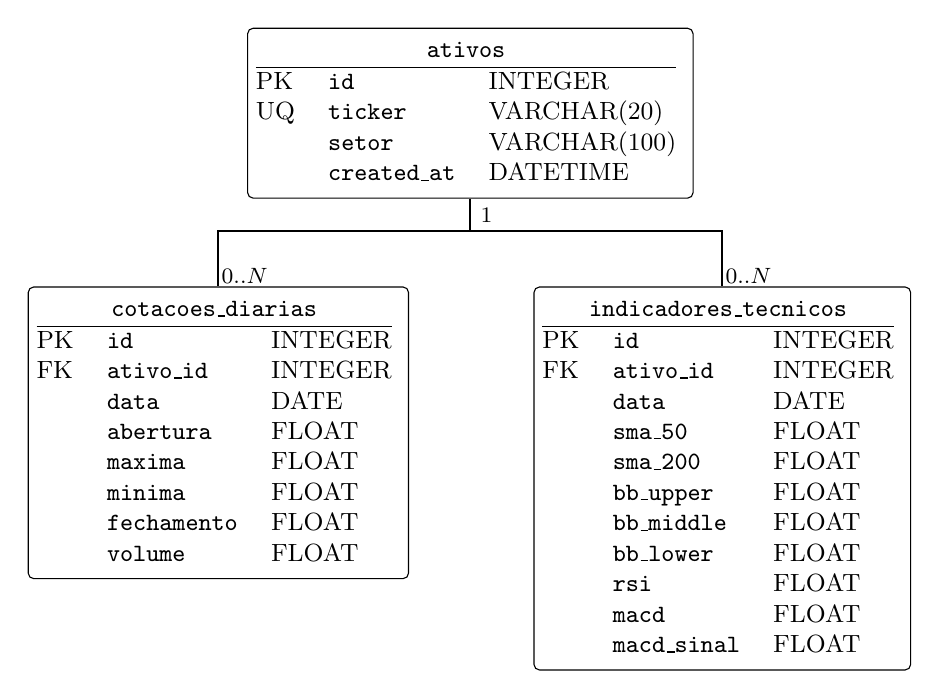
\begin{tikzpicture}[
  box/.style={draw, rounded corners=2pt, align=center, inner sep=3pt, font=\small},
  rel/.style={thick},
]
\node[box] (ativos) at (0,0) {
  \begin{tabular}{@{}lll@{}}
    \multicolumn{3}{c}{\textbf{\texttt{ativos}}}\\ \hline
    PK & \texttt{id}          & INTEGER\\
    UQ & \texttt{ticker}      & VARCHAR(20)\\
       & \texttt{setor}       & VARCHAR(100)\\
       & \texttt{created\_at} & DATETIME\\
  \end{tabular}
};
\node[box, anchor=north] (cotacoes) at (-3.2,-2.2) {
  \begin{tabular}{@{}lll@{}}
    \multicolumn{3}{c}{\textbf{\texttt{cotacoes\_diarias}}}\\ \hline
    PK & \texttt{id}          & INTEGER\\
    FK & \texttt{ativo\_id}   & INTEGER\\
       & \texttt{data}        & DATE\\
       & \texttt{abertura}    & FLOAT\\
       & \texttt{maxima}      & FLOAT\\
       & \texttt{minima}      & FLOAT\\
       & \texttt{fechamento}  & FLOAT\\
       & \texttt{volume}      & FLOAT\\
  \end{tabular}
};
\node[box, anchor=north] (indicadores) at (3.2,-2.2) {
  \begin{tabular}{@{}lll@{}}
    \multicolumn{3}{c}{\textbf{\texttt{indicadores\_tecnicos}}}\\ \hline
    PK & \texttt{id}          & INTEGER\\
    FK & \texttt{ativo\_id}   & INTEGER\\
       & \texttt{data}        & DATE\\
       & \texttt{sma\_50}     & FLOAT\\
       & \texttt{sma\_200}    & FLOAT\\
       & \texttt{bb\_upper}   & FLOAT\\
       & \texttt{bb\_middle}  & FLOAT\\
       & \texttt{bb\_lower}   & FLOAT\\
       & \texttt{rsi}         & FLOAT\\
       & \texttt{macd}        & FLOAT\\
       & \texttt{macd\_sinal} & FLOAT\\
  \end{tabular}
};

\coordinate (juncao) at (0,-1.5);
\draw[rel] (ativos.south) -- node[right, font=\footnotesize] {\(1\)} (juncao);
\draw[rel] (juncao) -| (cotacoes.north);
\draw[rel] (juncao) -| (indicadores.north);
\node[font=\footnotesize, fill=white, inner sep=1pt, above right] at (cotacoes.north) {\(0..N\)};
\node[font=\footnotesize, fill=white, inner sep=1pt, above right] at (indicadores.north) {\(0..N\)};
\end{tikzpicture}
\caption{Diagrama entidade-relacionamento do banco de dados de mercado do Hedge-fund-lab. PK indica chave primária, FK indica chave estrangeira e UQ indica restrição de unicidade. O par \texttt{(ativo\_id, data)} é único em cada tabela dependente.}
\label{fig:hfl-der}
\end{figure}

O livro contábil das carteiras (identidade \texttt{HFL-MANUAL-PORTFOLIO-V1}) grava cada evento em uma tabela SQLite com gatilhos que recusam \texttt{UPDATE} e \texttt{DELETE}. As escritas usam \texttt{BEGIN IMMEDIATE} e \texttt{synchronous=FULL}. Valores monetários e quantidades são tratados com \texttt{Decimal} e arredondados a centavos pelo núcleo contábil reutilizado de \texttt{scripts/multiasset\_portfolio.py}.

\FloatBarrier
\section{Códigos de erro do relógio causal}

Os controles de causalidade descritos na Seção~\ref{sec:arq-relogio} interrompem a execução com os seguintes códigos:

\begin{itemize}
  \item \texttt{decision\_input\_lookahead}: a verificação preliminar das versões v2 e v3, executada sob bloqueio de rede (\texttt{no\_network()}), encontrou uma sessão de entrada igual ou posterior ao dia-alvo;
  \item \texttt{input\_changed\_before\_transport}: a entrada de um ativo, relida imediatamente antes da requisição HTTP, difere da versão registrada;
  \item \texttt{manager\_context\_changed\_before\_transport}: o mesmo para o contexto do gestor;
  \item \texttt{campaign\_identity\_changed}: já existe, na raiz da campanha, um manifesto diferente do que seria gravado (Seção~\ref{sec:arq-replay}).
\end{itemize}

\section{Reservas de orçamento e tarifas}

A reserva gravada antes de cada tentativa HTTP é de US\$~0,110592 por chamada de analista ou de risco e de US\$~0,159744 por chamada do gestor, valores calculados pelos limites de \textit{bytes} de entrada e \textit{tokens} de saída às tarifas mais altas anunciadas pelo provedor. Ao receber a resposta, o custo é estimado com US\$~0,75 por milhão de \textit{tokens} de entrada e US\$~3,75 por milhão de \textit{tokens} de saída e de raciocínio; sem uso válido, a reserva integral permanece contabilizada. Esperas de reenvio superiores a 30 segundos interrompem a execução. O controle é implementado em \texttt{scripts/continuous\_replay\_runtime.py}, é independente da estratégia e a auditoria correspondente (\texttt{audit\_budget}) está nos exportadores.

\section{Constantes da versão v3}

A Tabela~\ref{tab:constantes-v3} reúne as constantes determinísticas de \texttt{scripts/continuous\_replay\_v3.py} referidas na Seção~\ref{sec:arq-evolucao}.

\begin{table}[htbp]
\centering
\caption{Constantes determinísticas da versão v3.}
\label{tab:constantes-v3}
\small
\begin{tabular}{l r p{6.4cm}}
\toprule
\textbf{Constante} & \textbf{Valor} & \textbf{Função} \\
\midrule
\texttt{MAX\_ASSET\_WEIGHT} & 0,30 & Teto de peso projetado em compra por COMPRA \\
\texttt{DIP\_REBALANCE\_MAX\_WEIGHT} & 0,22 & Teto de peso em compra de recomposição em MANTER \\
\texttt{MIN\_TRADE\_BRL} & 2.000,00 & Valor bruto mínimo de compra (R\$) \\
\texttt{CORE\_FLOOR\_WEIGHT} & 0,08 & Peso mínimo remanescente após venda técnica normal \\
\texttt{MAX\_NORMAL\_SELL\_FRACTION} & 0,45 & Fração máxima da posição vendida por pregão \\
\texttt{ANTI\_WHIPSAW\_COOLDOWN\_SESSIONS} & 8 & Janela contra recompra mais cara (pregões) \\
\texttt{CASH\_DRAG\_THRESHOLD} & 0,25 & Caixa/patrimônio que habilita a recomposição \\
\texttt{STRENGTH\_TRIM\_MAX\_FRACTION} & 0,35 & Fração máxima de uma realização em força \\
\texttt{STRENGTH\_TRIM\_MIN\_WEIGHT\_AFTER} & 0,12 & Peso mínimo após realização em força \\
\texttt{TRIM\_MIN\_WEIGHT\_BEFORE}/\texttt{\_AFTER} & 0,25/0,15 & Limites do \textit{Trim-to-Fund}, herdados da v2 \\
\bottomrule
\end{tabular}
\end{table}

\section{Regras detalhadas das versões v2 e v3}

Esta seção detalha as regras resumidas na Seção~\ref{sec:arq-evolucao}.

\subsection{Versão v2}

A v2 acrescenta quatro intervenções, todas impostas tanto no \textit{prompt} do gestor (\texttt{PROMPT\_V2}) quanto no compilador (\texttt{compile\_proposal\_v2}):

\begin{itemize}
  \item \textbf{\textit{Trim-to-Fund}:} venda parcial de ativo com recomendação MANTER ou COMPRA, admitida quando o peso antes da operação supera 25\% do patrimônio, o peso projetado permanece em ao menos 15\% e a cesta contém uma compra válida ou o ativo já excede 30\%.
  \item \textbf{Teto de concentração e ordem mínima:} nenhuma compra pode levar o peso projetado do ativo acima de 30\% do patrimônio anterior à operação (\texttt{MAX\_ASSET\_WEIGHT}), nem ter valor bruto inferior a R\$~2.000,00 (\texttt{MIN\_TRADE\_BRL}); vendas não têm valor mínimo.
  \item \textbf{Veto assimétrico (R7):} o veredito \texttt{VETADO} passa a bloquear apenas compras; se o consenso técnico for VENDA, a recomendação permanece VENDA sob veto, permitindo reduzir ou zerar a posição.
  \item \textbf{Lentes analíticas:} cada analista recebe o \textit{prompt} técnico v5 acrescido de uma lente --- tendência estrutural (analistas 1 e 2), reversão por Bollinger e RSI (3 e 4) e regime de volatilidade como árbitro (5).
\end{itemize}

Além disso, o compilador deixa de invalidar o pregão diante de uma violação de regra: em modo não estrito, reduz a quantidade ou converte a ação em \texttt{HOLD} e registra cada ajuste com \textit{ticker}, lado, quantidades de origem e destino e o motivo (por exemplo, \texttt{MAX\_ASSET\_WEIGHT\_CAP}, \texttt{MIN\_TRADE\_BRL}, \texttt{TRIM\_WEIGHT\_AFTER\_FLOOR}). Violações estruturais --- universo incompleto ou com \textit{tickers} repetidos e quantidades inválidas --- continuam invalidando o pregão.

\subsection{Versão v3}

A v3 mantém as regras da v2 e acrescenta quatro grupos de mecanismos, parametrizados pelas constantes da Tabela~\ref{tab:constantes-v3}.

\begin{itemize}
  \item \textbf{Cinco lentes especialistas e travas de extremo.} Cada analista recebe uma lente única: Bandas de Bollinger, exaustão por RSI e MACD, valor relativo à média de 50 pregões, estrutura de longo prazo pela média de 200 pregões e assimetria entre o espaço até as bandas superior e inferior. Cada lente explicita faixas em que determinado sinal é proibido. Duas travas atuam apenas sobre consensos de exatamente três votos: \texttt{ANTI\_BOTTOM\_SELL\_GUARD} reverte VENDA para MANTER quando o RSI é inferior a 40 ou \texttt{bb\_lower\_gap} é inferior a 0,035, desde que \texttt{sma200\_gap} seja superior a $-0{,}08$; \texttt{ANTI\_TOP\_CHASE\_GUARD} reverte COMPRA para MANTER quando o RSI é superior a 62 ou \texttt{bb\_upper\_gap} é superior a $-0{,}02$.
  \item \textbf{Memória de posição, piso núcleo, venda escalonada e \textit{anti-whipsaw}.} O contexto do gestor passa a incluir, por ativo, a quantidade, o preço médio de compra, o retorno não realizado, a sessão e o preço da última venda e os pregões decorridos desde ela, reconstruídos do livro. Em venda técnica normal (VENDA com risco aprovado), o compilador limita a quantidade a 45\% da posição, arredondada para cima, e preserva peso remanescente de ao menos 8\% (ajuste \texttt{CORE\_FLOOR\_STEP\_SELL}); a saída integral fica restrita à venda sob veto (R7). É recusada a compra de ativo vendido nos últimos oito pregões a preço superior ao da última venda (\texttt{ANTI\_WHIPSAW\_HIGHER\_REBUY}).
  \item \textbf{\textit{Trim-on-Strength} e \textit{Trim-to-Fund}.} Além do \textit{Trim-to-Fund} da v2, admite-se a realização parcial em força de ativo em MANTER ou COMPRA quando ele está esticado (RSI $\geq$ 63 ou \texttt{bb\_upper\_gap} $\geq -0{,}02$), em lucro de ao menos 2\% sobre o preço médio e com peso acima de 14\%, limitada a 35\% da posição e a peso remanescente de 12\%, sem exigir compra na cesta.
  \item \textbf{Recomposição contra o arrasto de caixa (\textit{Dip-Rebalance}).} Quando o caixa do início do pregão supera 25\% do patrimônio, admite-se compra de ativo em MANTER com risco aprovado e em desconto (\texttt{sma50\_gap} negativo com RSI de até 46, ou \texttt{bb\_lower\_gap} de até 0,04), sujeita ao teto de 22\%, à ordem mínima e à regra \textit{anti-whipsaw}.
\end{itemize}



\chapter{Caminho de Ativo Único e Camada de Experimentos}
\label{ap:ativo-unico}

Este apêndice descreve o caminho de decisão de ativo único, construído para o protocolo confirmatório de ativo único (PETR4), planejado na etapa anterior para avaliar H2 (Seção~\ref{sec:met-protocolo}), e a camada de experimentos que o sustenta. Suas fases de desenvolvimento foram executadas, mas o Teste Final não; por isso o caminho não aparece nos resultados.

\section{Dados do protocolo de ativo único}

A série de PETR4 do protocolo vem de um \textit{snapshot} oficial do COTAHIST, ajustado pelo fator do \texttt{yfinance}, com 2.649 barras, uma por sessão oficial de 04/01/2016 a 31/08/2026. Dela, 1.519 sessões (de 12/01/2018 a 28/02/2024), cada uma com ao menos 504 sessões de histórico, formam o conjunto elegível de âncoras; quatro dessas sessões, escolhidas por quantis e sem olhar o mercado, compõem o conjunto de diagnóstico \texttt{H\_real}. O calendário de negociação (\texttt{B3Calendar}, em \path{src/backtesting/b3_calendar.py}) aplica as regras históricas de feriados da B3 e reproduz as 2.649 sessões oficiais.

\section{Indicadores, estratégias e motor de \textit{backtesting}}

Os indicadores técnicos são implementados em \texttt{src/indicators}: médias móveis simples (\texttt{sma.py}), Bandas de Bollinger (\texttt{bollinger.py}), Índice de Força Relativa (\texttt{rsi.py}, formulação canônica de Wilder) e MACD (\texttt{macd.py}).

As estratégias residem em \texttt{src/strategies}, com uma interface comum em \texttt{base.py}: \textit{Buy and Hold} (\texttt{buy\_and\_hold.py}), carteira igualmente ponderada (\texttt{equal\_weight.py}), cruzamento de médias móveis (\texttt{sma\_cross.py}), Bandas de Bollinger (\texttt{bollinger\_bands.py}), mínima variância (\texttt{min\_variance.py}) e o controle clássico da família de indicadores (\texttt{indicator\_family\_control.py}). Esse último combina SMA, Bandas de Bollinger, RSI e MACD em um escore discreto no conjunto $\{-1, 0, +1\}$, servindo de \textit{benchmark} clássico para a comparação com o sistema multiagente de ativo único. No caminho multiativos, \texttt{dashboard/rule\_portfolios.py} aplica \texttt{sma\_cross.py} (50/200) e \texttt{bollinger\_bands.py} (20 períodos, 2 desvios) a parcelas independentes de 20\% do capital por ativo, e as carteiras de pesos iguais e de mínima variância utilizam as classes \texttt{EqualWeightPortfolio} e \texttt{MinVariancePortfolio} de \texttt{src/backtesting/portfolio.py}.

O motor de \textit{backtesting} (\texttt{src/backtesting}) centraliza a simulação de carteiras, o cálculo de métricas e a incorporação de custos: \texttt{engine.py} conduz a simulação, \texttt{portfolio.py} modela a carteira, \texttt{costs.py} aplica custos de transação e \texttt{metrics.py} concentra as métricas de risco e retorno. O calendário (\texttt{b3\_calendar.py}) alinha as decisões às sessões oficiais. A integração com o sistema multiagente de ativo único é feita por \texttt{agent\_engine.py} e \texttt{daily\_agent.py}, que conectam as decisões dos agentes à execução simulada, e por \texttt{arena.py}, que organiza a comparação entre estratégias. A métrica primária de avaliação do sistema multiagente (\textit{Sharpe Ratio}) é definida de forma congelada em \texttt{metrics.py}, sob o identificador \texttt{H2\_SCIENTIFIC\_SHARPE\_DEFINITION\_V1}, cuja especificação é detalhada no Capítulo~\ref{cha:metodologia}. O Replay Contínuo multiativos não utiliza \texttt{engine.py}.

\section{Sistema multiagente de ativo único}
\label{sec:arq-ativo-unico}

A lógica de decisão de ativo único é modelada como um sistema multiagente coordenado pelo LangGraph, no módulo \texttt{src/agents}. O grafo é linear e acíclico (Figura~\ref{fig:grafo-langgraph}): os agentes são executados em sequência, sem debate cíclico nem reavaliação iterativa. Cada nó corresponde a um papel especializado, e as arestas definem a ordem de execução. A aresta condicional após o gestor de risco só encaminha a decisão ao gestor de portfólio quando o veredito consolidado é \texttt{APROVADO}.

\begin{figure}[htbp]
\centering
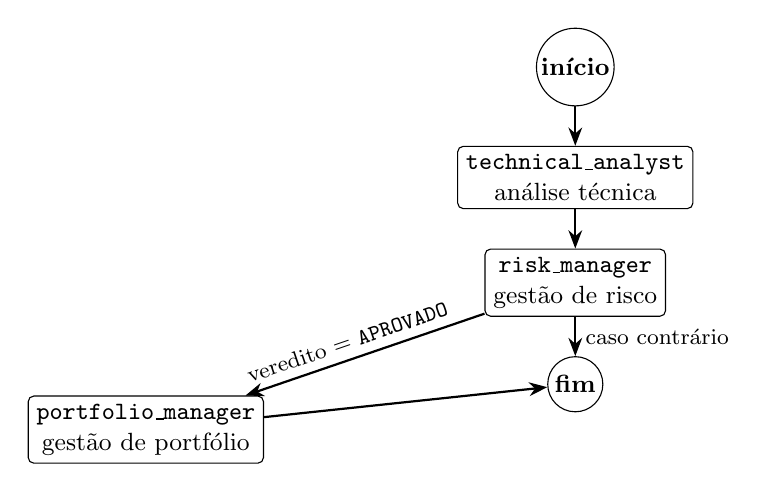
\begin{tikzpicture}[
  node distance=5mm,
  box/.style={draw, rounded corners=2pt, minimum height=7mm, align=center, inner sep=3pt, font=\small},
  term/.style={draw, circle, minimum size=7mm, align=center, font=\small\bfseries, inner sep=1pt},
  arr/.style={-Stealth, thick},
]
\node[term] (start) {início};
\node[box, below=of start] (ta) {\texttt{technical\_analyst}\\análise técnica};
\node[box, below=of ta] (rm) {\texttt{risk\_manager}\\gestão de risco};
\node[box, below left=10mm and 28mm of rm] (pm) {\texttt{portfolio\_manager}\\gestão de portfólio};
\node[term, below=of rm] (end) {fim};
\draw[arr] (start) -- (ta);
\draw[arr] (ta) -- (rm);
\draw[arr] (rm) -- node[above, sloped, pos=0.55, font=\footnotesize] {veredito = \texttt{APROVADO}} (pm);
\draw[arr] (pm) -- (end);
\draw[arr] (rm) -- node[right, font=\footnotesize] {caso contrário} (end);
\end{tikzpicture}
\caption{Grafo de decisão do caminho de ativo único (LangGraph): sequência linear \texttt{technical\_analyst} $\rightarrow$ \texttt{risk\_manager}, com aresta condicional ao \texttt{portfolio\_manager} apenas quando o veredito é \texttt{APROVADO}.}
\label{fig:grafo-langgraph}
{\footnotesize Fonte: elaborado pelos autores, a partir de \path{src/agents/graph.py}.}
\end{figure}

Os papéis são três. O agente de análise técnica (\texttt{technical\_analyst.py}) interpreta os indicadores quantitativos e emite uma recomendação inicial. O agente de gestão de risco (\texttt{risk\_manager.py}), amparado por um contrato de risco (\texttt{risk\_contract.py}), avalia a exposição e pode restringir a decisão. O agente de gestão de portfólio (\texttt{portfolio\_manager.py}) consolida as análises e define a decisão final. Na configuração científica, a direção da decisão é determinada pelo comitê e a exposição é atribuída por peso-alvo determinístico, sem dimensionamento dinâmico de posição pelo gestor de portfólio; o modo legado de dimensionamento por confiança permanece no código apenas como alternativa experimental.

O estado compartilhado do grafo é definido em \texttt{state.py}; as \textit{features} e sua semântica, em \texttt{features.py} e \texttt{feature\_semantics.py}; a evidência técnica apresentada aos agentes, em \texttt{technical\_evidence.py}; e os \textit{prompts} de análise técnica, em \texttt{technical\_prompt\_v4.py} e \texttt{technical\_prompt\_v5.py}. A comunicação com o modelo é encapsulada em \texttt{llm\_client.py}, com rastreamento em \texttt{llm\_trace.py}, e cada participante do comitê é representado em \texttt{participant.py}. O método de decisão é o \textit{self-consistency}, em que múltiplos analistas votam e a decisão consolidada exige um limiar de consenso com voto obrigatório de todos os participantes; a configuração congelada é apresentada no Capítulo~\ref{cha:metodologia}.

O grafo (\texttt{build\_graph}, em \path{src/agents/graph.py}) é utilizado pelos participantes da arena experimental e pelos executores de ativo único (\texttt{scripts/run\_agent\_backtest.py}, \texttt{scripts/run\_agent\_daily.py}). O participante recusa universos com mais de um ativo, e seu estado mantém posição escalar, caixa e patrimônio de um único papel. Por essa razão, a carteira multiativos não instancia o grafo: reutiliza o nó do comitê técnico e os esquemas de resposta de \texttt{src/agents}, mas substitui o gestor de risco e o gestor de portfólio por papéis próprios.

\section{Camada de experimentos e proveniência}
\label{sec:arq-experimentos}

A execução e o controle dos experimentos de ativo único concentram-se em \texttt{src/experiments}. O módulo \texttt{spec.py} define a especificação do experimento; \texttt{runner.py} conduz a execução; \texttt{hardening.py}, \texttt{cal\_b.py}, \texttt{stress.py} e \texttt{phases.py} implementam as fases do desenho experimental; \texttt{anchors.py} define as âncoras temporais; \texttt{treatment.py} e \texttt{context.py} organizam o tratamento e o contexto de cada execução; e os módulos \texttt{h2\_evaluation.py}, \texttt{h2\_evaluation\_offline.py}, \texttt{h2\_evaluation\_production.py} e \texttt{h2\_evaluation\_manifest.py} tratam da avaliação do sistema multiagente e da geração do manifesto de proveniência.

A reprodutibilidade é garantida por um conjunto de identificadores registrados a cada execução: o \textit{commit} do código, o \textit{hash} da especificação (\texttt{spec\_hash}), o identificador do \textit{snapshot} de dados, o manifesto de execução e o rastreio das chamadas ao modelo de linguagem. As fases e os identificadores de caso não fazem parte do \texttt{spec\_hash}, de modo a não vincular a especificação a uma janela temporal específica.

O caminho multiativos reutiliza dessa camada o diário durável de chamadas (\texttt{CallBank} e \texttt{DurableGeminiClient}, de \texttt{h2\_evaluation\_production.py}) e o bloqueio de rede (\texttt{no\_network}, de \texttt{h2\_evaluation\_offline.py}), com identidades próprias, sem alterar os \textit{gates} do protocolo de ativo único. Sua proveniência é registrada nos manifestos de campanha e nos pacotes descritos no Apêndice~\ref{ap:empacotamento}.

\chapter{Empacotamento e Publicação das Campanhas}
\label{ap:empacotamento}

Este apêndice detalha o mecanismo de identidade, artefatos, exportação e publicação das campanhas do Replay Contínuo, resumido na Seção~\ref{sec:arq-replay}.

\section{Executores, manifestos e \textit{lock}}

Cada geração possui um executor próprio: \texttt{scripts/continuous\_replay.py} (identidade \texttt{HFL-CONTINUOUS-EXPLORATORY-REPLAY-V1}), \texttt{scripts/continuous\_replay\_v2.py} (\texttt{-V2}) e \texttt{scripts/continuous\_replay\_v3.py} (\texttt{-V3}), cada um com raiz de armazenamento, livro, orçamento e pacote exportado próprios. As versões v2 e v3 conferem o \textit{hash} do \textit{bundle} de mercado antes do uso e reutilizam contabilidade, livro, planejador, transporte e orçamento por vinculação de módulo (\texttt{pilot\_paper.bind}). O \textit{bundle} da campanha (\texttt{inputs/market.json} e \texttt{inputs/manifest.json}) é gerado por \texttt{scripts/continuous\_replay\_data.py}.

No início de cada execução, o executor monta um manifesto com a identidade, o modo (inferência real ou teste \textit{offline}), as sessões, as estratégias, as políticas de referência, o teto de orçamento e os \textit{hashes} SHA-256 de todas as fontes. Um manifesto diferente na raiz recusa a execução (\texttt{campaign\_identity\_changed}). A v1 copia ainda os módulos de livro, proventos e regras para uma pasta imutável da campanha (\texttt{engine/}) e confere, por \textit{hash}, que as estratégias SMA/Bollinger e de portfólio importadas coincidem com essas cópias. Um \textit{lock} exclusivo impede dois executores simultâneos sobre a mesma raiz. As referências podem ser produzidas isoladamente (\texttt{-{}-references-only}). Na mínima variância, o otimizador SLSQP tem a função-objetivo dividida por um escalar positivo (a maior variância da diagonal), o que preserva o minimizador e as restrições; o eventual recurso aos pesos iguais também fica registrado no recibo de decisão. O aquecimento dos indicadores não cria patrimônio anterior ao início da campanha.

\section{Artefatos por pregão}

Para cada pregão, o executor grava na pasta da sessão, nesta ordem: \texttt{before.json} (estado das carteiras antes do pregão, após o crédito dos proventos pagos até a referência); \texttt{result.json} ou \texttt{failure.json} (resultado do comitê de cada ativo, com a entrada e o diário de chamadas); \texttt{context.json} e \texttt{proposal.json} (contexto e proposta compilada do gestor); \texttt{execution.json} (plano de execução); e \texttt{day.json} (fechamento do dia, com a marcação das seis carteiras). Cada comitê e cada gestor possuem um diário de chamadas (\texttt{CallBank}), exportado como \texttt{provider\_journal.jsonl}. A auditoria do orçamento (\texttt{audit\_budget}) reconstrói todas as tentativas, confere o \textit{hash} de cada envelope e recalcula o custo a partir dos \textit{tokens}.

\section{Exportadores}

Os exportadores (\texttt{scripts/export\_continuous\_replay.py}, \texttt{\_v2.py} e \texttt{\_v3.py}) leem os recibos já gravados, sem inferência nem alteração do livro, e produzem: \texttt{explorer.json} com as sessões, carteiras, pareceres e operações; \texttt{calls.json} com as chamadas arquivadas; tabelas CSV de patrimônio diário, operações, decisões, proventos e chamadas; uma página HTML autônoma com Chart.js embutido e um carregador das chamadas sob demanda (\texttt{calls-data.js}), gerados pelo próprio exportador nas versões v2 e v3 e por \texttt{scripts/build\_replay\_explorer.py} na v1; e um \texttt{manifest.json} selado com o \textit{hash} da exportação e o resultado da auditoria de orçamento. O conjunto é distribuído como pacote ZIP.

\section{Publicação e rotas}

A instalação no servidor é feita por \texttt{scripts/publish\_replay.py}, que aceita apenas o pacote cujo SHA-256 está fixado no código para cada versão e com a lista exata de membros esperada. Os arquivos são extraídos em área temporária, conferidos e promovidos por renomeação no mesmo volume; um destino existente só é aceito se seus arquivos coincidirem com o pacote, e dados diferentes nunca são sobrescritos. Cada versão ocupa um diretório próprio, preservando as anteriores.


A consulta é servida pelas rotas \path{/laboratory/replay/}, \path{/laboratory/replay/v2/} e \path{/laboratory/replay/v3/} de \texttt{dashboard/server.py}, somente com leitura: o servidor entrega apenas uma lista fechada de dez arquivos exportados, confina o caminho ao diretório da versão, comprime as respostas grandes sob demanda e não executa agentes nem operações. O explorador compara as curvas das seis carteiras e permite inspecionar, por carteira e pregão, posições, votos, pareceres de risco, decisões, operações, proventos e as chamadas arquivadas ao modelo. Os textos produzidos pelos modelos são apresentados como evidência preservada, não como fatos verificados.


\end{document}
